%% LyX 2.3.2-2 created this file.  For more info, see http://www.lyx.org/.
%% Do not edit unless you really know what you are doing.
\documentclass[english]{upeeei}
\usepackage[latin9]{inputenc}
\setcounter{secnumdepth}{3}
\setcounter{tocdepth}{3}
\usepackage[active]{srcltx}
\usepackage{float}
\usepackage{units}
\usepackage{graphicx}
\usepackage{textcomp}

%Added libraries aside from default ones
\usepackage{pgfgantt}
\usepackage{circuitikz}
\usepackage{amsmath}
\usepackage{stackengine}
\usepackage{breqn}
\usepackage{pgfplots}
\tikzset{voltage dir=RP}
\usepackage{url}
\usepackage{subfig}
\usepackage{algorithm}
\usepackage{algpseudocode}

% Some of the article customisations are relevant for this class

\usepackage{tikz}
\usetikzlibrary{shapes.geometric,arrows.meta,fit,positioning}
\usepackage{caption}
\definecolor{blue1}{RGB}{143,33,53}
\definecolor{gray}{RGB}{232,232,232}
\definecolor{gray1}{RGB}{92,92,92}
\definecolor{black}{RGB}{0,0,0}
\definecolor{white}{RGB}{255,255,255}
\tikzstyle{startstop} = [rectangle, rounded corners, minimum width=3cm, minimum height=1cm,text centered, draw=none, fill=blue1, text = gray]
\tikzstyle{io} = [trapezium, trapezium left angle=70, trapezium right angle=110, minimum width=3cm, minimum height=1cm, text centered, draw=none, fill=blue!30]
\tikzstyle{filler} = [rectangle, rounded corners, minimum width=3cm, minimum height=1cm,text centered, draw=none, fill=white, text = black]
\tikzstyle{process} = [rectangle, minimum width=3cm, minimum height=1cm, text centered, draw=none, text width = 3cm,fill=orange!30]
\tikzstyle{decision} = [diamond, minimum width=3cm, minimum height=1cm,text width=3 cm, text centered, draw=none, fill=green!30]
\tikzstyle{arrow} = [thick,->,>=fast cap]
\tikzstyle{arrow_cap} = [-Triangle, line width=1.5pt,draw=gray1]
\tikzset{fit margins/.style={/tikz/afit/.cd,#1,
    /tikz/.cd,
    inner xsep=\pgfkeysvalueof{/tikz/afit/left}+\pgfkeysvalueof{/tikz/afit/right},
    inner ysep=\pgfkeysvalueof{/tikz/afit/top}+\pgfkeysvalueof{/tikz/afit/bottom},
    xshift=-\pgfkeysvalueof{/tikz/afit/left}+\pgfkeysvalueof{/tikz/afit/right},
    yshift=-\pgfkeysvalueof{/tikz/afit/bottom}+\pgfkeysvalueof{/tikz/afit/top}},
    afit/.cd,left/.initial=2pt,right/.initial=2pt,bottom/.initial=2pt,top/.initial=2pt}
\makeatletter

%%%%%%%%%%%%%%%%%%%%%%%%%%%%%% LyX specific LaTeX commands.
\providecommand{\LyX}{L\kern-.1667em\lower.25em\hbox{Y}\kern-.125emX\@}
%% Because html converters don't know tabularnewline
\providecommand{\tabularnewline}{\\}

\@ifundefined{showcaptionsetup}{}{%
 \PassOptionsToPackage{caption=false}{subfig}}
\usepackage{subfig}
\renewcommand{\ALG@name}{Pseudocode}
\makeatother

\usepackage{babel}
%\pgfplotsset{compat=1.17}
\begin{document}

%%% UP EEEI undergraduate project template
%% v0.1 by Louis P. Alarcon 11/22/2011
%%
%% LyX template - use with the following files:
%% 	uct10_new.clo, uct11_new.clo, uct12_new.clo, upeeei.cls, upeeei.layout
%%
%% Place project title here
\title{Implementation of Parallel-1D FDTD Algorithm using Schwarz Alternating Method} 

%%
%% Author information

\author{
%% Louis Poblete Alarc\'on\\ xxxx-xxxxx\\ \emph{Ph.D. Electrical Engineering and Computer Sciences} \and
Karlo Pio Dungog Alaan\\ 2015-07559\\ \emph{B.S. Electronics and Communications Engineering}\\and\\
 Jan Marvin Delos Reyes Moyco\\ 2015-09359\\ \emph{B.S. Electronics and Communications Engineering}\and
}

%%
%% Month and year of submission/graduation
\degreeyear{2021} 
\degreesemester{August} 

% Put your advisers here:
\chair{Adrian Vidal} 
\othermembers{Jaybie Agullo De Guzman\\ Bernalyn Decena} 
\numberofmembers{2} 

\field{Electrical/Computer/Electronics and Communications Engineering} 
\campus{Diliman} 

\maketitle 
% \approvalpage 
% \copyrightpage 
\begin{abstract} 

%Your abstract goes here...
% In a \emph{single} well-written paragraph, this is what we'd like to do.  Try to cover Need, Solution, Differentiation, Benefit (NSDB).  Use the content of this template as an example for formatting your proposal document, \textbf{NOT} as a strict guide for the flow of your discussion and what your proposal must contain.

Students predominantly have no access to powerful computational devices when doing electromagnetic simulations. These usually require powerful hardware because of the scale and complexities of the problems. Finite Difference Time Domain (FDTD) is one of the popular numerical methods for solving electromagnetic problems because of its simplicity and ease of implementation. Parallel FDTD algorithms have already shown significant advantage over traditional serial FDTD algorithms but they lack a method of validating the data in each subdomain. Schwarz Alternating method is a common domain decomposition method used in solving partial differential equations. A new method combining the a parallelized FDTD via the Schwarz method is developed in this project. This can narrow the gap between the lack of access to powerful hardware and the need for electromagnetic simulations by utilizing parallel computing with relatively inexpensive hardware. The current progress of the project is the development of a serial 1D FDTD algorithm in Python.




\abstractsignature\end{abstract}

\begin{frontmatter} 

\setlength{\parskip}{0pt}

\tableofcontents{}

\listoffigures

\listoftables

\end{frontmatter} 

\def\MASTERDOC{true}

\cleardoublepage{}

\chapter{Introduction\label{cha:Introduction}}



\section{Background of the Project}\label{sec:bg}

In 2020, the COVID-19 pandemic forced every educational institution in the world to forego face-to-face classes and moved its operations online. This change in mode of learning exacerbated already existing problems of students with the lack of devices for learning or research as well as internet connectivity. Before the pandemic began, data from Philippine Statistics Authority \cite{PSA2020} show that less than 30\% of households in the Philippines have access to a desktop or laptop. During the pandemic, an estimated 6.8 million students lack access to proper Information and Communications Technologies (ICT) devices (phone, tablet, laptop, etc) for online learning and 6.8 million lack access to a stable internet connection in the Philippines \cite{Mateo2020}. Another survey conducted by Social Weather Stations shows that only 13\% of enrolled Filipino students have access to a desktop or laptop \cite{CNN2021} which is usually needed for tech-related or engineering courses. This lack of access to computing resources are apparent despite the decrease in the price of computers in recent years.\\

These problems are more apparent in tertiary education since in general, college students need some sort of ICT devices for their studies. For example, in a survey conducted by UP Media and Public Relations Office, 28\% students in the UP System do not have access to any ICT device for learning \cite{Abrogar2020} while majority of the students in UP Diliman (approximately 97\% of the total student population) have some sort of access to an internet connection \cite{USC2020} as shown on Figure  \ref{fig:student-survey}.\\ 

\begin{figure}[H]
    \centering
    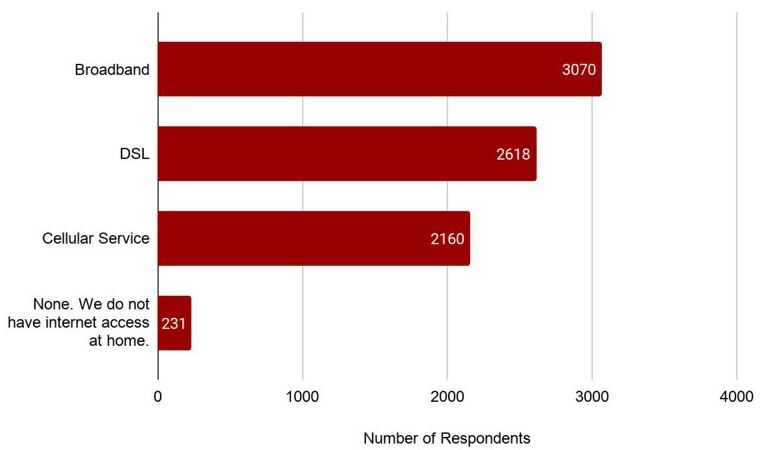
\includegraphics[width=\textwidth]{images/student_internet_survey.JPG}
    \caption{The internet sources of the respondents in the survey shows that most students have access to an internet connection in different forms \cite{USC2020}.}
    \label{fig:student-survey}
\end{figure}



One of the methods used to increase accessibility to computational resources without acquiring expensive hardware is cloud computing \cite{Queensland2017}. This is a type of computing where the computing resources can be rented on-demand without buying any hardware \cite{AWS} can offload the burden of acquiring new hardware, maintaining the hardware, and upgrading the hardware while retaining the computational resources at a fraction of the cost \cite{Armbrust2009}.  This will be advantageous to anyone without access to high computational resources because renting computing power is much lower than acquiring and maintaining hardware that provides the same computing power. This advantage is especially beneficial in processes that involves large amounts of data processing like electromagnetic (EM) simulations because of the need for high computational power in a short period of time, cloud computing can be used to augment the researcher's computational needs in a certain amount of time without spending a large amount and tweaking the hardware to suit research requirements. \\


In EM research, simulating and modelling EM events is usually difficult to do because current problems in EM research need complex design and large structure to provide adequate solutions \cite{Wolff2016} and require long simulation time. In addition, EM problems that has real world application rarely has exact analytical solution and using approximate solutions from numerical methods that are tailored for solving Maxwell's Equation are the next best thing \cite{RumpfCEM}. There are several methods of computing Maxwell's equations numerically like Finite Difference Time Domain (FDTD) \cite{Toroglu2014}, Finite Element Method (FEM) \cite{Haldar2006}, Method of Moment (MoM) \cite{Arvas2012}, etc. FDTD, in particular, has been a very popular tool for EM simulations \cite{Ramadan2017} due to its ease of implementation and good accuracy of the simulation \cite{Wolff2016}.\\

To improve the long simulation time issue common in complex EM problems, parallel computing can be integrated to the simulation of EM problems. Parallel computing is the method of splitting a  numerical problem into several sub-problems such that  the computation of each sub-problem can be done simultaneously \cite{Karniadakis2003}. This method improves the simulation time of an EM problem because of the simultaneous processing of each part of the main problem. The computational load on each sub problem is less than the total problem so in theory, a problem can be solved without investing too much on high performance processors. \\

Overall, cloud computing can be used to minimize the cost of EM research due to the hardware requirements while parallel computing can reduce the simulation time of complex EM problems. Thus, combining FDTD with parallel processing and cloud computing can be a good solution in creating an efficient, accurate, and accessible system for EM simulations.\\


\section{Project Overview }

\begin{figure}[H]
    \centering
    %
\includegraphics{images/fdtd_major steps.JPG}
    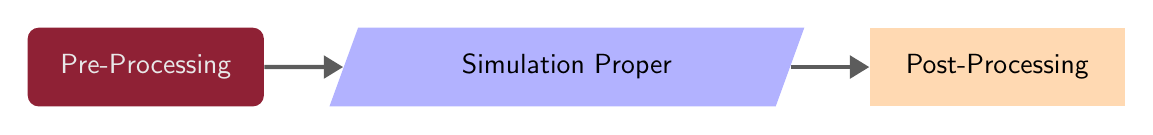
\begin{tikzpicture}
	\sffamily
	%Creating elements in the tikz picture
	\node (pre_process) [startstop] {Pre-Processing};
	\node (sim_proper) [io, right= of pre_process] {Simulation Proper};
	\node (post_process) [process, right = of sim_proper] {Post-Processing};

	%Drawing arrows
	\draw [arrow_cap] (pre_process) -- (sim_proper);
	\draw [arrow_cap] (sim_proper) -- (post_process);

    \end{tikzpicture}
    \caption{Block Diagram for the EEE 190 Project}
    \label{fig:blk_diagram}
\end{figure}

The building blocks of the project shown in Figure \ref{fig:blk_diagram} are the major components of the project:

\begin{enumerate}
    \item \textbf{Pre-Processing} - is the part where the input data is processed, simulation parameters are initialized (creation of variables and computing constants), and the computational domain is created for the simulation proper.
    \item \textbf{Simulation Proper} - is where the proposed algorithm will be used and the necessary measurements are done.
    \item \textbf{Post-Processing} - is the part where the data is consolidated for analysis, data visualization, and storage.
\end{enumerate}



%Pre-Processing -> Simulation Proper (FDTD + Schwarz) -> Post Processing

\section{Documentation Flow and Organization}

In the succeeding chapters, the review of related works will explain the relevant concepts that will be used in the project. The problem statement and objectives explains the project's scope as well as expected objectives at the project completion. The methodology is the detailed explanation of how the project will be accomplished as well as the method of verification of the results. The initial simulation results of the project will be presented in the preliminary findings and the project schedule and deliverables will discuss the timeline of the project as well as the deliverables and their relation to the project's objectives.



\cleardoublepage{}

\chapter{Finite-Difference Time Domain}\label{cha:FDTD}

This chapter will focus on the basics of the Finite-Difference Time Domain method. It aims to familiarize the reader with the foundations of the method, starting with Maxwell's equations. From there, the Finite Difference method was used to approximate the equations for easier numerical solving. The basic FDTD algorithm is also shown in this chapter. Lastly, the derivation of the one-dimensional FDTD is presented here as well. 


\section{Maxwell's Equations}
Maxwell's equations are the foundation of electromagnetic theory. The equations are shown in Equation \ref{Maxwell's Eqns}. 

\begin{subequations}\label{Maxwell's Eqns}
    \begin{align}
        \nabla \cdot \mathbf{D} &= \rho_v &\text{Gauss' Law}\\
        \nabla \cdot \mathbf{B} &= 0 &\text{Gauss' Law for Magnetism}\\
        \nabla \times \mathbf{H} &= \mathbf{J} + \frac{\partial \mathbf{D}}{\partial t} &\text{Ampere's Law}\\
        \nabla \times \mathbf{E} &= -\frac{\partial \mathbf{B}}{\partial t} &\text{Faraday's Law of Induction}
    \end{align}
\end{subequations}


% Equation \ref{Maxwell's Eqns}a is the first Maxwell Equation or Gauss' Law, which states that electric fields must move outward from a positive charge and conversely, the electric field must move inward to a negative charge. Gauss' law also states that if there are no electric charges, the electric field will form loops. \cite{Rumpf2014}.

% The second Maxwell Equation, Equation \ref{Maxwell's Eqns}b, or Gauss' Law for magnetism states that that there can be no magnetic monopoles \cite{Jackson1999}, and that magnetic fields will always form loops. 

% Equation \ref{Maxwell's Eqns}c is Maxwell's third equation or Ampere's Law, which states that "circulating magnetic fields induce currents and/or time-varying electric fields" \cite{Rumpf2014}. Conversely, it also states that "currents and/or time varying electric fields induce circulating magnetic fields". \cite{Rumpf2014}. 

% The fourth Maxwell equation, Equation \ref{Maxwell's Eqns}d, or Faraday's Law of Induction states that circulating electric fields induce time-varying magnetic fields. Conversely, time varying magnetic fields induce circulating electric fields \cite{Rumpf2014}. 

\section{Finite Difference Method}\label{FD method}

Both Curl Equations consist of derivatives. Since computers cannot inherently solve for derivatives, some approximations can be made for them to calculate derivatives. The Finite Difference Method is used to get an appropriate approximation for the Curl Equations.

The Finite Difference Method calculates the derivative at the midpoint of two points of a function. In approximating the Curl Equations, special care must be given when formulating the approximated equations. Particularly, each term of both sides of the equation must exist in at the same point in time. This is to ensure that the equations are stable during the simulations \cite{Rumpf2020.1}. 

Using the Finite Difference Method, the Curl Equations can be approximated as shown in Equations \ref{Maxwell approx1} and \ref{Maxwell approx2}. 

\begin{align}
        \label{Maxwell approx1}
        \nabla \times \mathbf{E} = -\frac{\partial \mathbf{B}}{\partial t} \quad &\Rightarrow \quad \nabla \times \mathbf{E}(t+\Delta t) \simeq -\mu \frac{\mathbf{H}(t+\frac{\Delta t}{2})-\mathbf{H}(t-\frac{\Delta t}{2})}{\Delta t}\\
    \label{Maxwell approx2}
    \nabla \times \mathbf{H} = \frac{\partial \mathbf{D}}{\partial t} \quad &\Rightarrow \quad \nabla \times \mathbf{H}(t+\frac{\Delta t}{2}) \simeq \varepsilon \frac{\mathbf{E}(t+\Delta t)-\mathbf{E}(t)}{\Delta t}
\end{align}

From the above equations, another set of equations called the Update Equations can be defined. These equations will be used to compute the field values at the next time step inside the FDTD loop. The Update Equations can be seen in Equation \ref{update eqs}. 

\begin{subequations}\label{update eqs}
    \begin{align}
        \left.\mathbf{H}\right|_{t+\frac{\Delta t}{2}} &= \left.\mathbf{H}\right|_{t-\frac{\Delta t }{2}}-\frac{\Delta t}{\mu }\left(\nabla \times \left.\mathbf{E}\right|_{t}\right)\\
        \left. \mathbf{E}\right|_{t+\Delta t} &= \left.\mathbf{E}\right|_t + \frac{\Delta t}{\varepsilon}\left(\nabla \times \left.\mathbf{H}\right|_{t+\frac{\Delta t}{2}}\right)
    \end{align}
\end{subequations}

\section{The Basic FDTD Algorithm}

The type of FDTD used in this project is the Alternating Direction Implicit (ADI) since it has less stringent stability criterion \cite{Namiki1999}. The basic operating principle of the FDTD algorithm is the leapfrog method \cite{Rumpf2014}. It uses values from another field to compute the values of the current field. In FDTD, the electric field is computed based on the magnetic field, and conversely, the magnetic field is computed based on the electric field. This cycle continues until the set number of iterations is finished. 

The FDTD algorithm updates the values of the fields via the Update equations in \ref{update eqs}. The basic FDTD algorithm flowchart can be seen in Fig. \ref{fig:basic_fdtd}. In order to reduce computation time, constants such as the time step and permittivity can be initialized at the beginning. Both fields are also initialized to zero. 

\begin{figure}[H]
    \centering
    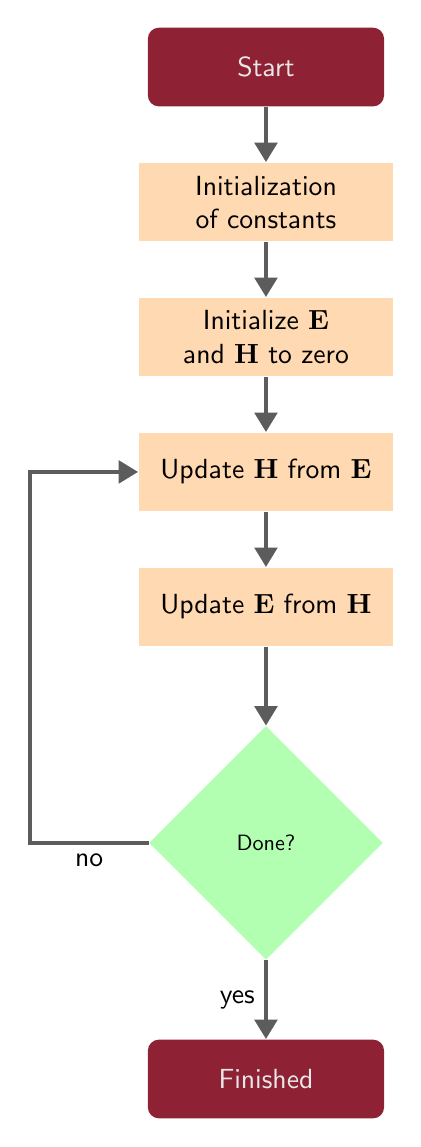
\begin{tikzpicture}
	\centering
	\sffamily
	%Creating the elements in the FDTD Flowchart
	\node (start) [startstop] {Start};
	\node (init) [process, below= of start, yshift=0.3cm] {Initialization of constants};
	\node (init2) [process, below= of init, yshift=0.3cm] {Initialize $\mathbf{E}$ and $\mathbf{H}$ to zero};
	\node (update1) [process, below=of init2, yshift=0.3cm] {Update $\mathbf{H}$ from $\mathbf{E}$};
	\node (update2) [process, below=of update1, yshift=0.3cm] {Update $\mathbf{E}$ from $\mathbf{H}$};
	\node (done) [decision, below = of update2, scale=0.8] {Done?};
	\node (finish) [startstop, below = of done] {Finished};

	%Draw the arrows for the flowchart
	\draw [arrow_cap] (start) -- (init);
	\draw [arrow_cap] (init) -- (init2);
	\draw [arrow_cap] (init2) -- (update1);
	\draw [arrow_cap] (update1) -- (update2);
	\draw [arrow_cap] (update2) -- (done);
	\draw [arrow_cap] (done) -- node[anchor=east] {yes} (finish);
	\draw [arrow_cap] (done) -- node[anchor=north] {no} ++(-3,0) |-  (update1.west);
	
    \end{tikzpicture}
    \caption{Basic FDTD Algorithm}
    \label{fig:basic_fdtd}
\end{figure} 

\section{Reduction to 1D Using Yee Grid Scheme}
The Equations in \ref{FD method} deal with the time components of Maxwell's Curl Equations. However, these equations still exist in three dimensions. In compliance to the objectives of this project, these equations need to be reduced to one dimension only. This can be achieved using Yee Cells \cite{Rumpf2020.1}. 

Yee cells are used to discretize the space components of the Curl Equations. In a Yee cell, the electric and magnetic fields are arranged such that they are staggered inside the grid \cite{Yee1998}. A visual representation of the Yee cell with the fields can be seen in Figure \ref{fig:Yee cell} \cite{Rumpf2020.1}. 

\begin{figure}[H]
    \centering
    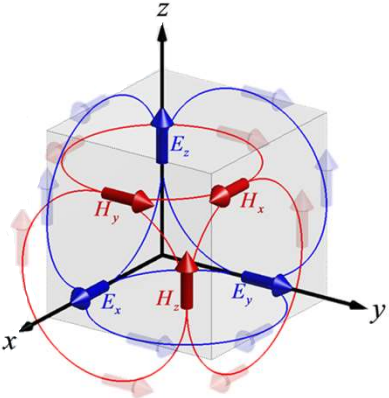
\includegraphics[scale=0.5]{images/Yee cell.png}
    \caption{Three-dimensional Yee Cell \cite{Rumpf2020.1}.}
    \label{fig:Yee cell}
\end{figure}

Equations for the $x$, $y$, and $z$ components of the Curl Equations can be deduced from one Yee cell. However, the derivations will no longer be included in this document for the purpose of conciseness. The focus is shifted towards the reduced one-dimensional Yee cell, as shown in Figure \ref{fig:1D Yee cell} \cite{Rumpf2020.1}. There are two configurations or modes of the one-dimensional Yee cell: the $E_y/H_x$ mode and the $E_x/H_y$ mode. For this project, the $E_y/H_x$ mode will be used since the two are functionally the same. As seen in the figure, only the $y$ component of the electric field remains, while only the $x$ component of the magnetic field remains.


\begin{figure}[H]
    \centering
    \subfloat[\centering $E_y/H_x$ mode]{{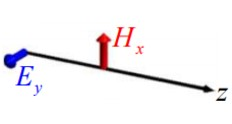
\includegraphics[width=5cm]{images/Ey_Hx .jpg} }}%
    \qquad
    \subfloat[\centering $E_x/H_y$ mode]{{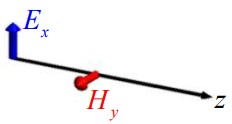
\includegraphics[width=5cm]{images/Ex_Hy.jpg} }}
    \caption{One-dimensional Yee cells \cite{Rumpf2020.1}.}
    \label{fig:1D Yee cell}
\end{figure}

The $E_y/H_x$ mode is possible since the derivatives along \( x \) and \( y \) computed using the three-dimensional analysis can be reduced to zero. The field values along those directions are constant since material properties only change along the propagation path, which is the $ z $ direction. The Curl Equations can be reduced as seen in Equation \ref{reduced curl}, where $k$ is the array index.  

\begin{subequations}\label{reduced curl}
    \begin{align}
    -\frac{\textbf{E}_y^{k+1}(t)-\textbf{E}_y^k(t)}{\Delta z } &= \frac{\mu^k}{c_0} \frac{\textbf{H}_x^k(t+\frac{\Delta t}{2})-\textbf{H}_x^k(t-\frac{\Delta t}{2})}{\Delta t}\\
    \frac{\textbf{H}_x^k(t+\frac{\Delta t}{2})-\textbf{H}_x^{k-1}(t+\frac{\Delta t}{2})}{\Delta z} &= \frac{\varepsilon^k}{c_0}\frac{\textbf{E}_y^k(t+\Delta t)-\textbf{E}_y^k(t)}{\Delta t}
    \end{align}
\end{subequations}

Using Equation \ref{reduced curl}, a more refined set of the Update Equations can be derived, specifically for the $E_y/H_x$ mode. The new equations can be seen in Equation \ref{update eqs2}, and will be used for the entirety of the project. 

\begin{subequations}\label{update eqs2}
    \begin{align}
        \left. \textbf{E}_y^k \right|_{t+\Delta t} &= \left. \textbf{E}_y^k \right|_{t} + \left(\frac{C_0 \Delta t}{\varepsilon^k}\right) \left(\frac{\left.\textbf{H}_x^k\right|_{t+\frac{\Delta t}{2}}-\left. \textbf{H}_x^{k-1}\right|_{t+\frac{\Delta t}{2}}}{\Delta z}\right)\\
        \left.\textbf{H}_x^k\right|_{t+\frac{\Delta t}{2}} &= \left.\textbf{H}_x^k\right|_{t-\frac{\Delta t}{2}} - \left(\frac{C_0 \Delta t}{\mu^k}\right)\left(\frac{\left.\textbf{E}_y^{k+1}\right|_t-\left.\textbf{E}_y^k\right|_t}{\Delta z}\right)
    \end{align}
\end{subequations}

\section{More Detailed 1D FDTD} \label{subsec:fdtd_method}

The scope for this project is to use a FDTD in one dimension, which is the simplest type of FDTD that can be used to show if the parallel configuration is better than serial configuration. The most basic algorithm of FDTD is the leapfrog method \cite{Rumpf2014} that alternates in solving for the electric and magnetic field in each Yee cell using the update equations \cite{Houle2019}. The update equations used in this project are the Ey/Hx form of the FDTD Update equation in 1D \cite{Rumpf082014} and this form is chosen arbitrarily since the other form Ex/Hy is similar to the Ey/Hx form. The difference is the convention of the directions of the electric and magnetic fields in the simulation space.


\begin{align}
    &\tilde{\textbf{H}}_x|^{k}_{t+\frac{\Delta t}{2}}\,=\,\tilde{\textbf{H}}_x|^{k}_{t-\frac{\Delta t}{2}}\,+\,(m_{\textbf{H}_x}|^k)(\frac{\textbf{E}_{y}|_{t}^{k+1}\,-\,\textbf{E}_{y}|_{t}^{k}}{\Delta z})\label{eq:updateH}\\
    &\textbf{E}_{y}|^{k}_{t+\Delta t}\,=\,\textbf{E}_{y}|^{k}_{t}\,+\,(m_{\textbf{E}_y}|^k)(\frac{\tilde{\textbf{H}}_x|_{t+\frac{\Delta t}{2}}^{k}\,-\,\tilde{\textbf{H}}_x|_{t+\frac{\Delta t}{2}}^{k-1}}{\Delta z})\label{eq:updateE}\\
    &m_{\textbf{E}_y}|^{k}\,=\,\frac{c_0 \Delta t}{\epsilon _{yy}|^{k}}\label{eq:update_coeffE}\\
    &m_{\textbf{H}_x}|^{k}\,=\,\frac{c_0 \Delta t}{\mu _{xx}|^{k}}
    \label{eq:update_coeffH}
\end{align}

The equation above shows the update equations and the update coefficients for both the electric and magnetic fields for the FDTD algorithm. There are two important points about the update equations that need to be discussed: their dependence on previous value and adjacent values. First, the first term in the update equation is the previous field value (for both electric and magnetic field) so, every value in the k-th position in space is dependent on the previous time step. Second, the dependence on adjacent cells, since the electric field has a term for the magnetic field in k-1 position, this means that the electric field is dependent on the adjacent magnetic field value while the magnetic field is dependent on the adjacent electric field value (because it has an electric field in k+1 position).



\begin{figure}[H]
    \centering
    %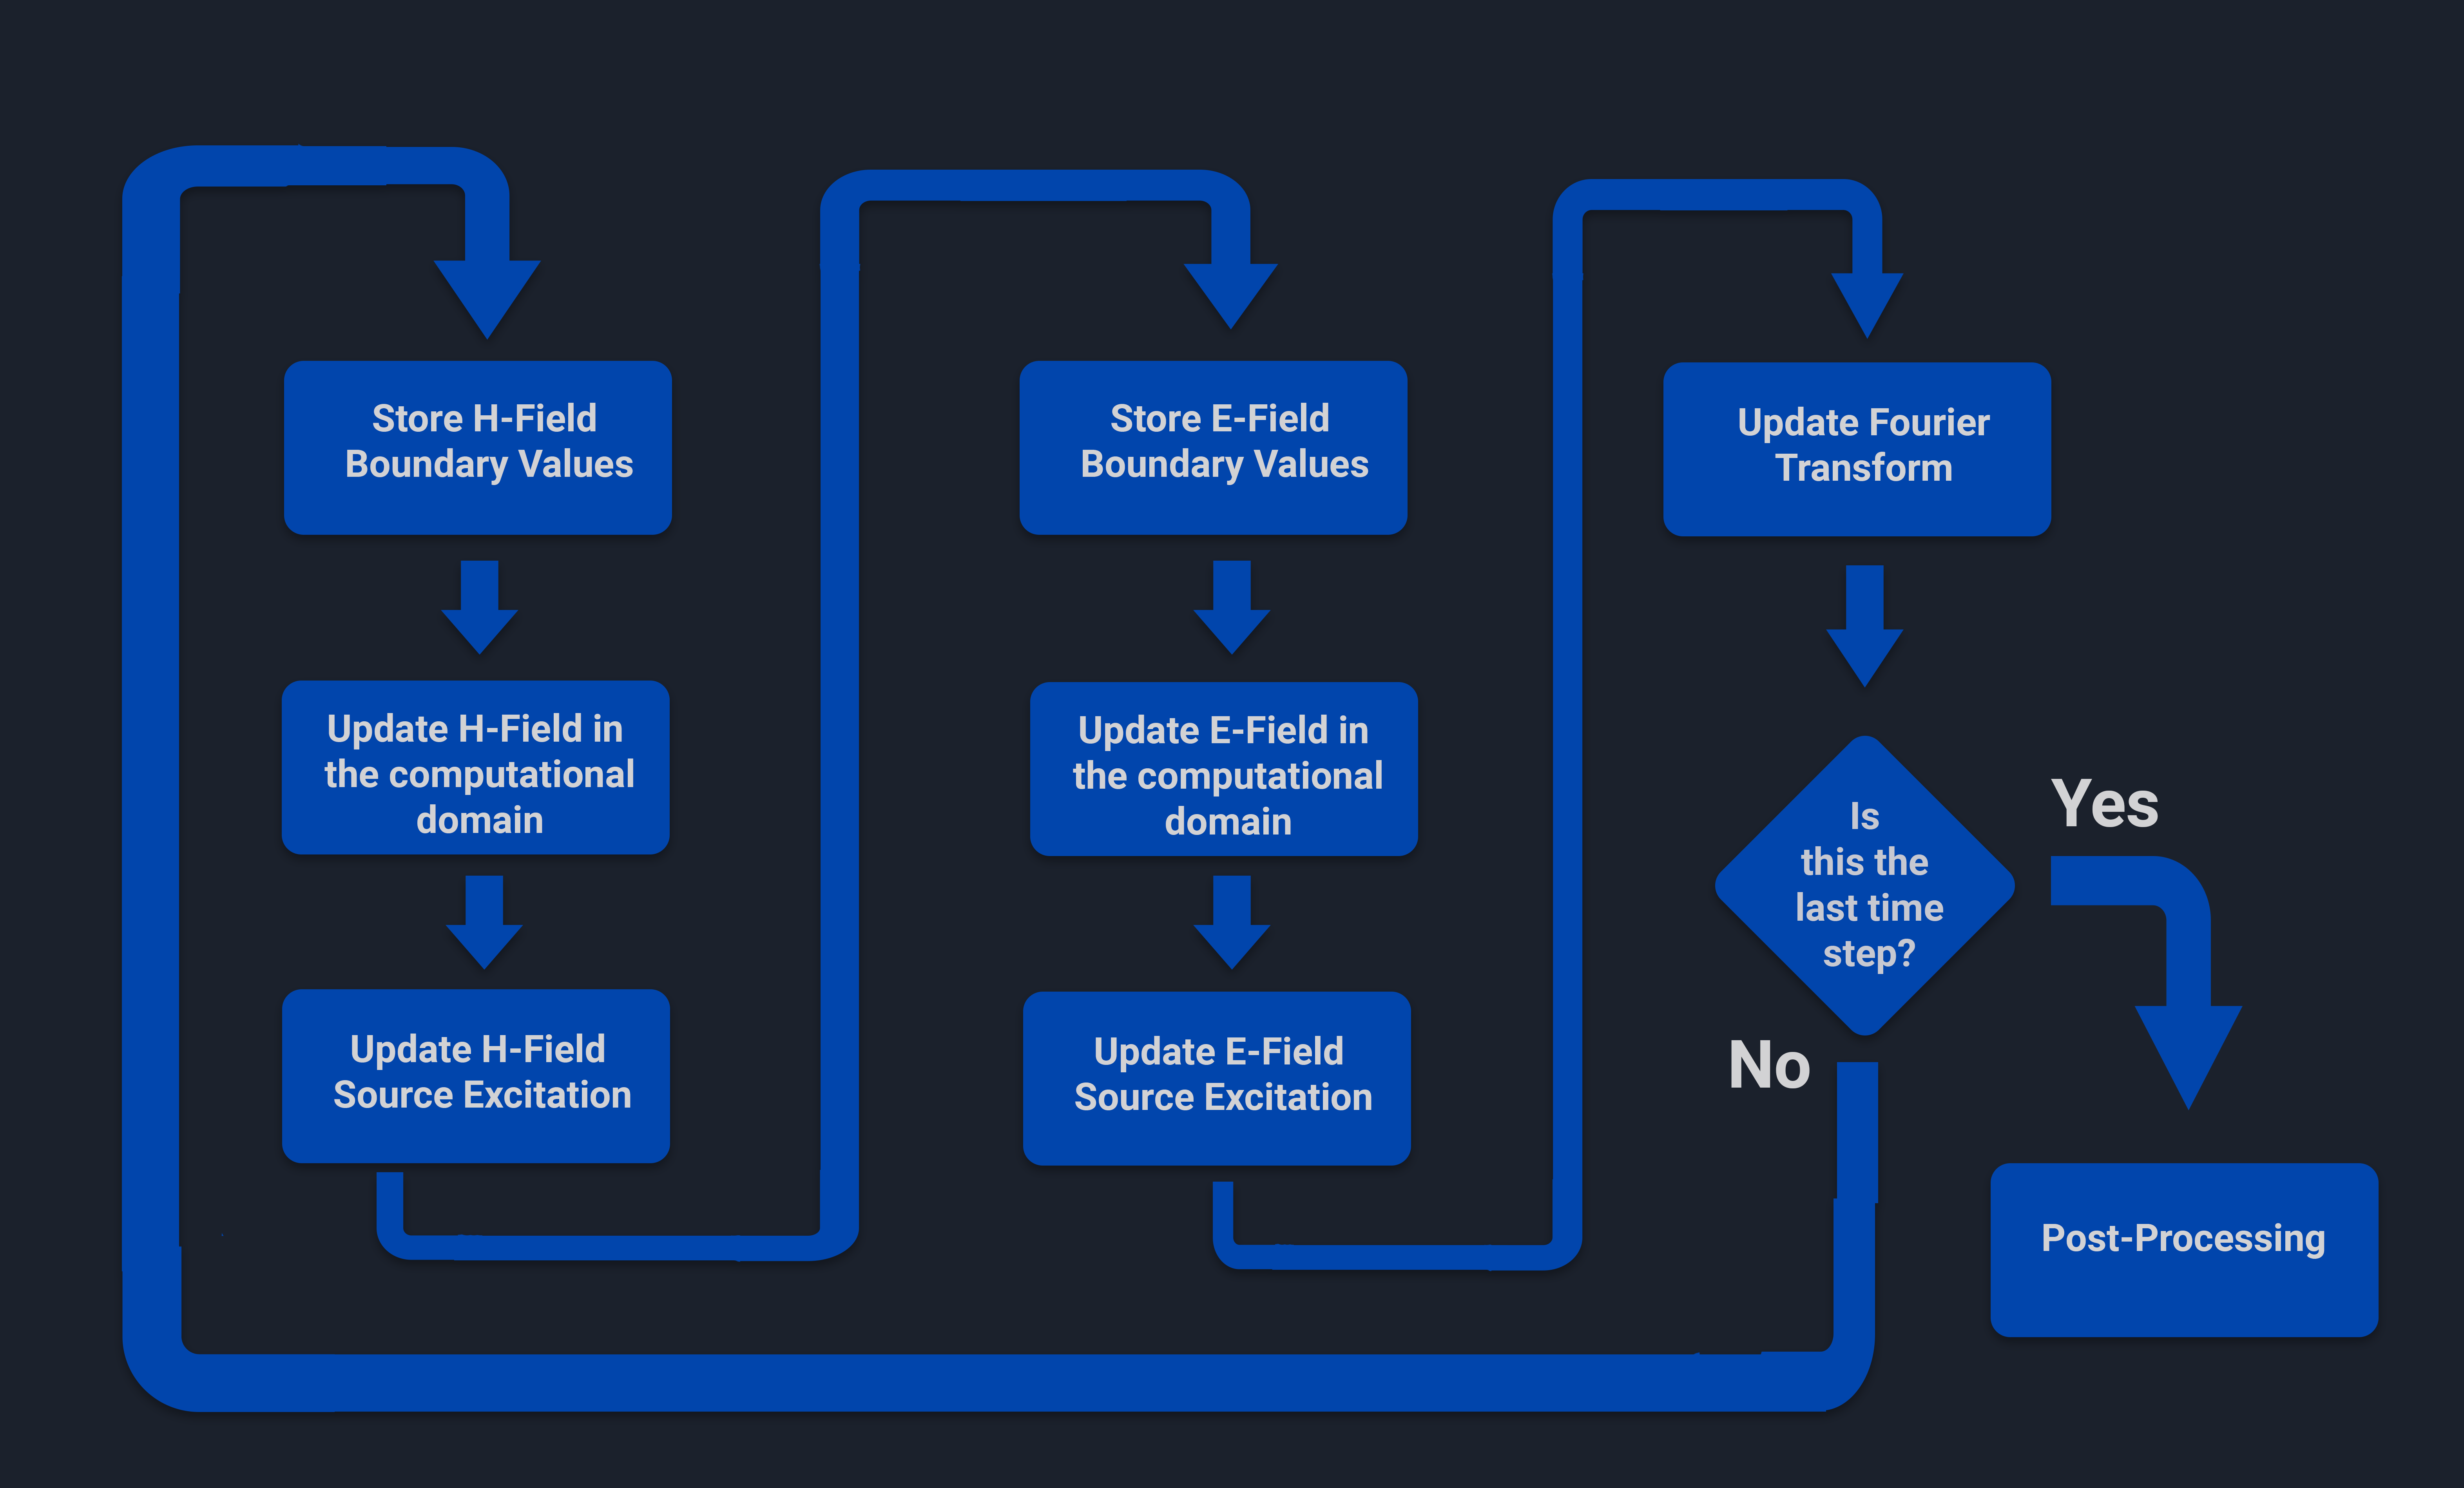
\includegraphics[width=\textwidth]{images/fdtdloop.png}
    \resizebox{!}{17cm}{
    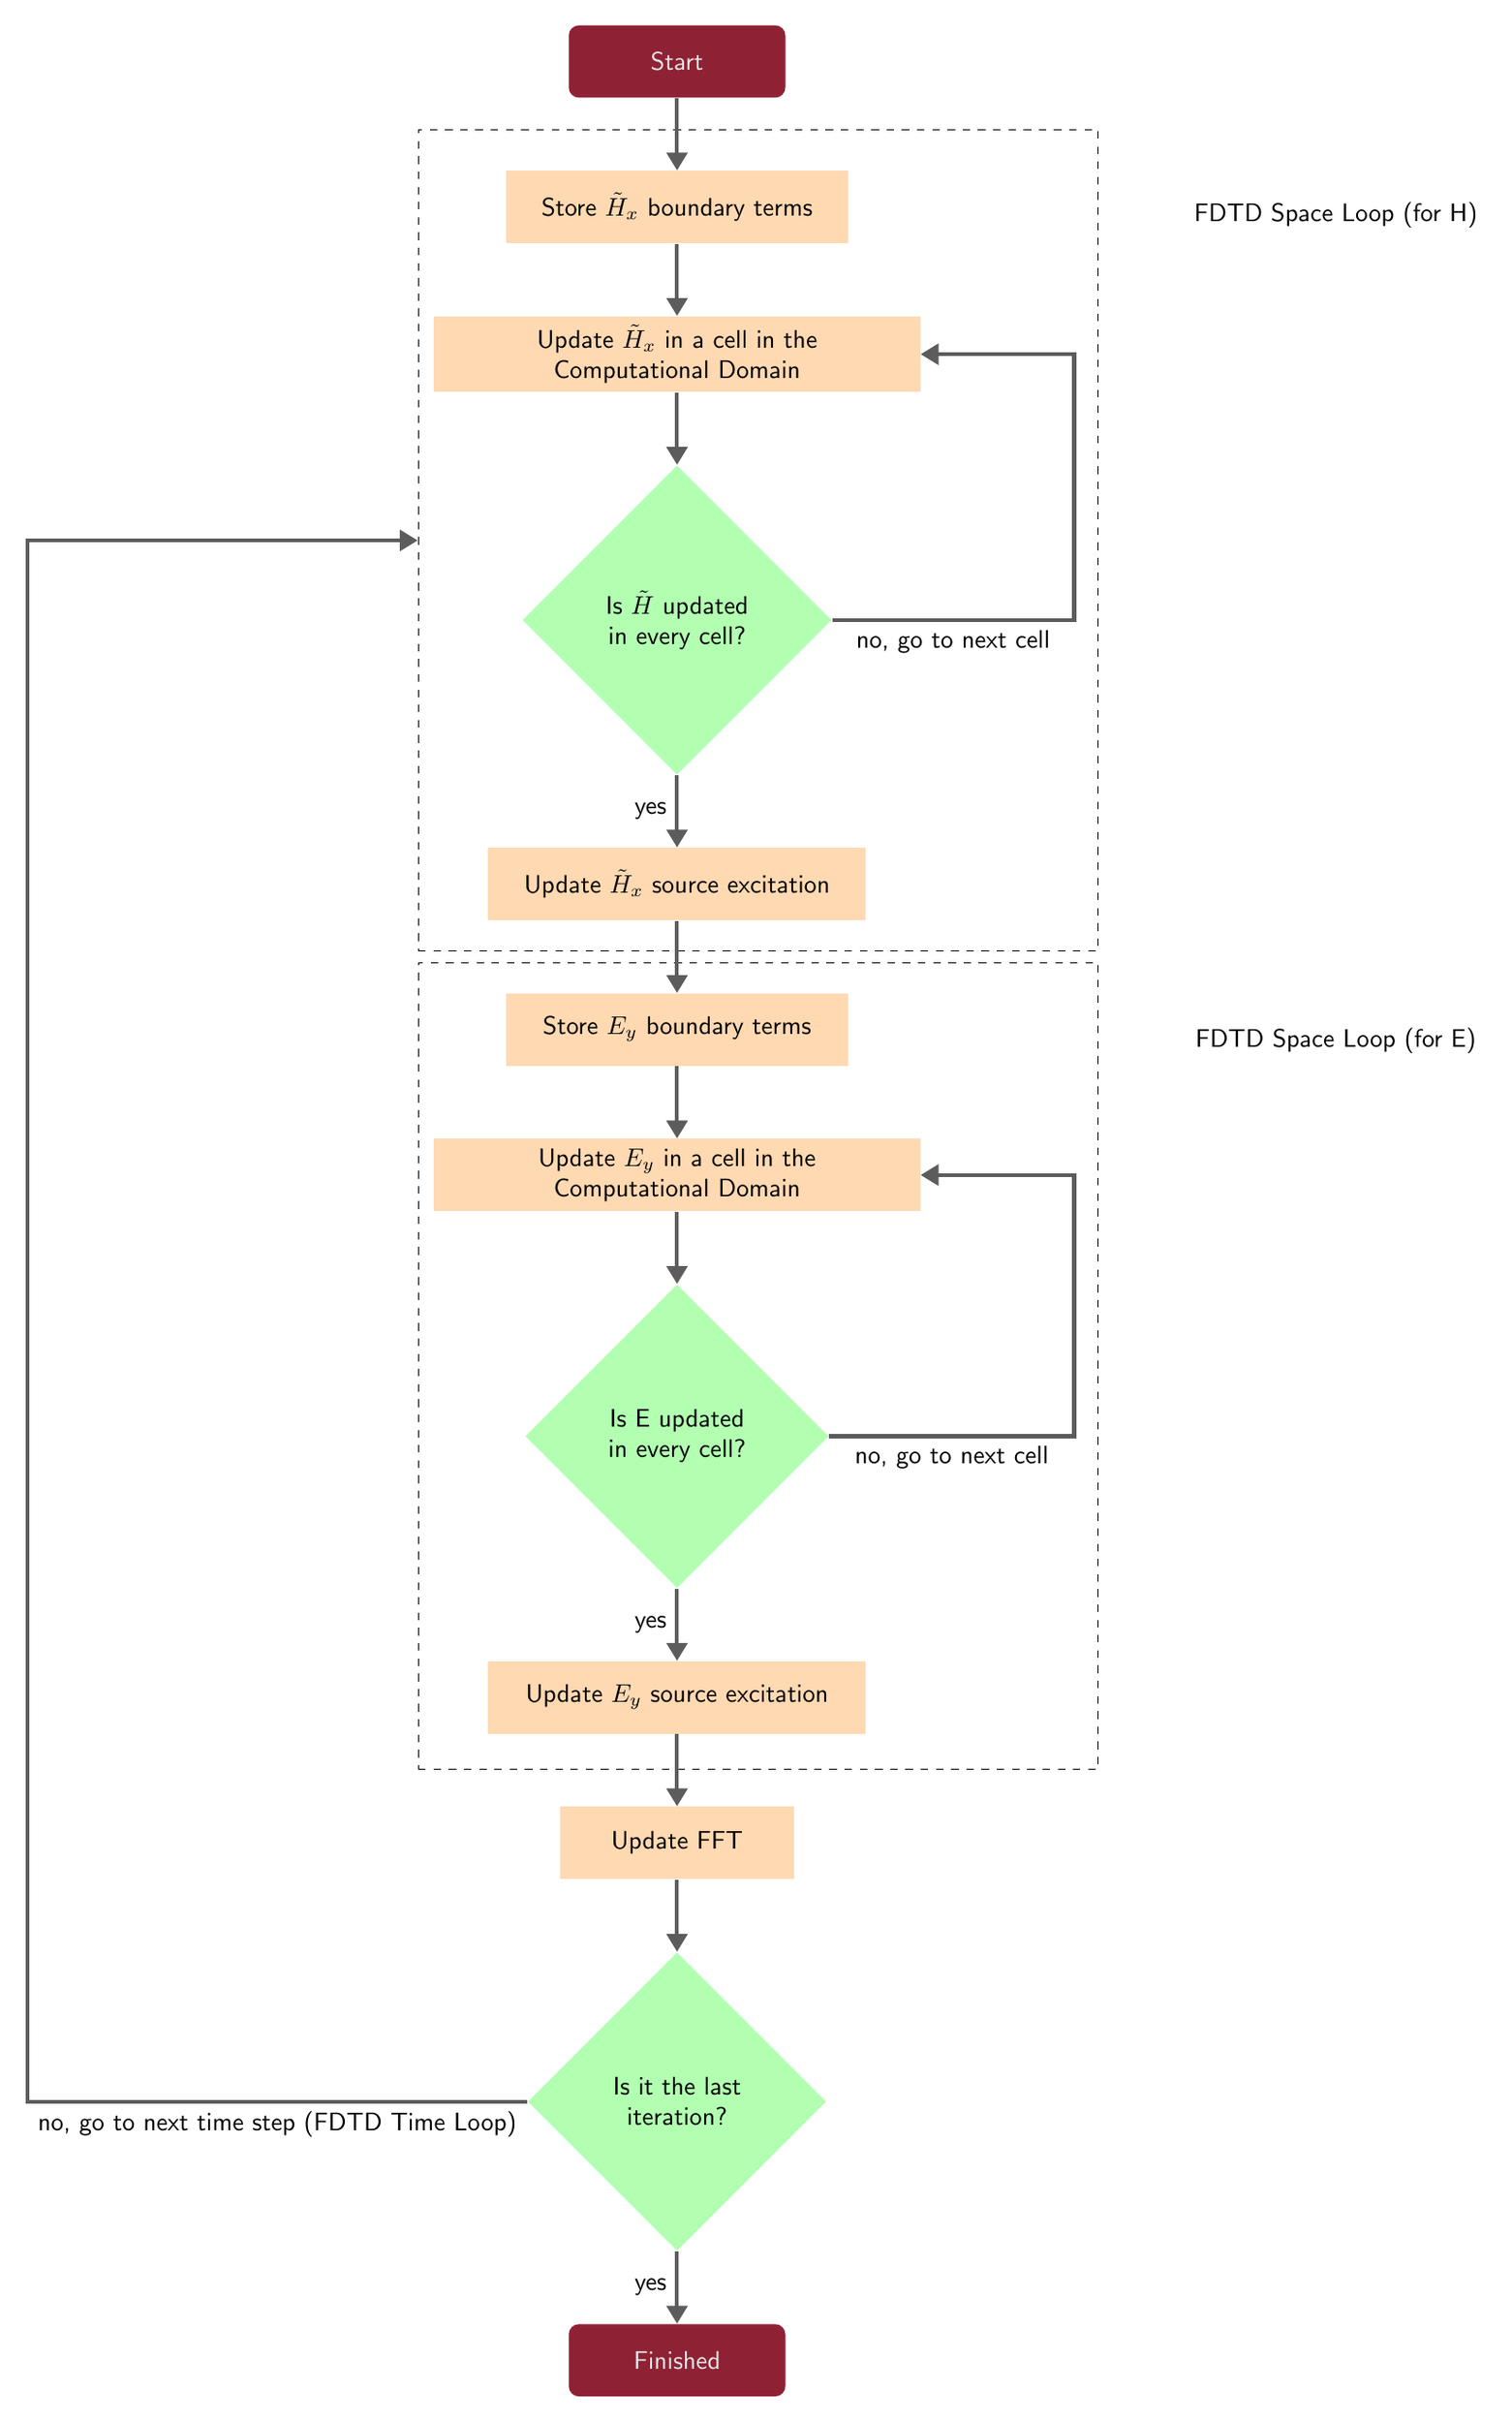
\begin{tikzpicture}
	\centering
	\sffamily
	%Creating the elements in the FDTD Flowchart
	\node (pre_process) [startstop] {Start};
	\node (store_Hboundary_terms) [process, text width=4.5cm, below=of pre_process] {Store $\tilde{H}_x$ boundary terms};
	\node (update_H) [process, text width=6.5cm, below= of store_Hboundary_terms] {Update $\tilde{H}_x$ in a cell in the Computational Domain};
	\node (is_H_finished) [decision, below= of update_H] {Is $\tilde{H}$ updated in every cell?};
	\node (update_source_H) [process, text width=5cm, below= of is_H_finished] {Update $\tilde{H}_x$ source excitation};
	\node (store_Eboundary_terms) [process, text width=4.5cm, below=of update_source_H] {Store $E_y$ boundary terms};
	\node (update_E) [process, text width=6.5cm, below= of store_Eboundary_terms] {Update $E_y$ in a cell in the Computational Domain};
	\node (is_E_finished) [decision, below= of update_E] {Is E updated in every cell?};
	\node (update_source_E) [process, text width=5cm,below= of is_E_finished] {Update $E_y$ source excitation};
	\node (update_FFT) [process, below = of update_source_E] {Update FFT};
	\node (last_iter) [decision, below = of update_FFT] {Is it the last iteration?};
	\node (post_process) [startstop, below = of last_iter] {Finished};

    \node[fit={ (store_Hboundary_terms)
	            (update_H)
	            (update_source_H)
                (is_H_finished)}, dashed, draw, fit margins={left=3pt,right=35pt,bottom=6pt,top=8pt} ] (fdtd_space_H){};
    \node  (fdtd_space_H_title) at ([shift={(8,4.5)}]fdtd_space_H) {FDTD Space Loop (for H)};
    \node[fit={ (update_E)
                 (update_source_E)
                 (store_Eboundary_terms)
                (is_E_finished)}, dashed, draw,fit margins={left=3pt,right=35pt,bottom=7pt,top=6pt} ] (fdtd_space_E){};
    \node  (fdtd_space_E_title) at ([shift={(8,4.5)}]fdtd_space_E) {FDTD Space Loop (for E)};


	%Draw the arrows for the flowchart
	\draw [arrow_cap] (pre_process) -- (store_Hboundary_terms);
	\draw [arrow_cap] (store_Hboundary_terms) -- (update_H);
	\draw [arrow_cap] (update_H) -- (is_H_finished);
	\draw [arrow_cap] (is_H_finished) -- node[anchor=east] {yes} (update_source_H);
	\draw [arrow_cap] (is_H_finished) --  node[anchor=north] {no, go to next cell} ++(5.5,0) |- ++(0,3)   |- (update_H.east);
	\draw [arrow_cap] (update_source_H) -- (store_Eboundary_terms);
	\draw [arrow_cap] (store_Eboundary_terms) -- (update_E);
	\draw [arrow_cap] (update_E) -- (is_E_finished);
	\draw [arrow_cap] (is_E_finished) -- node[anchor=east] {yes} (update_source_E);
	\draw [arrow_cap] (update_source_E) -- (update_FFT);
	\draw [arrow_cap] (is_E_finished) --  node[anchor=north] {no, go to next cell} ++(5.5,0) |- ++(0,3)   |- (update_E.east);
	\draw [arrow_cap] (update_FFT) -- (last_iter);
	\draw [arrow_cap] (last_iter) -- node[anchor=east] {yes} (post_process);
	\draw [arrow_cap] (last_iter) --  node[anchor=north] {no, go to next time step
	(FDTD Time Loop)} ++(-9,0) |- ++(0,15.5)   |- (fdtd_space_H.west);

    \end{tikzpicture}
    }
    \caption{1D FDTD Algorithm}
    \label{fig:fdtd_flowchart}
\end{figure} 


The flowchart shown in Fig \ref{fig:fdtd_flowchart} is the main algorithm of FDTD that computes for the field values in space and time. There are other steps like the pre-processing and post-processing that will be discussed in the implementation part of this chapter. In general, the FDTD algorithm has two main loops: the main loop that iterates through every time step, which will be referred here as the FDTD time loop and the inner loop that iterates through every cell in the computational domain, referred here as the FDTD space loop.

First, the FDTD time loop is where the main steps of the algorithm are done. There are three main steps: 

\begin{enumerate}
    \item Updating the magnetic field values
    \item Updating the electric field values
    \item Updating the Fourier Transform and checking the stop condition
\end{enumerate}

The first and second steps are similar, the only difference is what field values are updated. This first two step can be referred to as FDTD space loop since these steps are looping in the computational space of the simulation. The initial step in this part is to store the boundary values of magnetic or electric fields for the computation of the boundary condition in the next step. Next, to update the field values in the computational domain including the external boundary conditions of the domain, the FDTD space loop is involved since the iteration will be done through every cell in the computational domain. The update equation specified in \ref{eq:updateE} and \ref{eq:updateH} will be used to update each cell and after updating the cells in the whole computational domain.

The injection of source excitation is done after the update equations are done where the source excitation (computed in the pre-processing stage) will be used by injecting, depending on the method of excitation into the specified injection point ($k_{inj}$). This will affect the field values since the field values have a dependence on the adjacent cells and so, the effect of the source excitation will be seen after the current iteration in the FDTD time loop is finished. The method on how the source excitation is injected into $k_{inj}$ and what types of sources will be used in the project will be discussed in the implementation part.


After the storing of boundary values of the electric and magnetic fields, FDTD space loop for electric and magnetic fields, the last step in the FDTD time loop is the update of Fourier transform and checking of the stop condition. The  Fourier transform of each iteration in the FDTD time loop can be used to compute for the reflection and transmission coefficients for a specified frequency since FDTD is a time-based method, a single simulation run can include a wide range of frequencies \cite{Rumpf082014}. The equation used for calculating the reflection and transmission coefficients are shown below:

\begin{align}
    &R(f)\,=\,(\frac{FFT[E_{ref}(t)]}{FFT[E_{src}(t)]})^{2}\\
    &T(f)\,=\,(\frac{FFT[E_{trn}(t)]}{FFT[E_{src}(t)]})^2\\
    &C(f)\,=\,R(f)\,+\,T(f)
\end{align}

The reflected and transmitted fields are converted into the frequency domain by Fast Fourier Transform, and the fields are normalized with respect to the source excitation. The law of conservation of energy is also checked by getting the sum of the reflected and transmitted fields \cite{Rumpf082014}. This equation holds true in this situation because in the current FDTD model, the conductivity or the absorption loss after passing through a material is not taken into account so there should be no loss of energy because of the conductivity of the materials. The reflected and transmitted fields are measured at the first and last cells of the computational domain for the reflected and transmitted fields respectively. 

The stop condition for the FDTD time loop is when the current iteration reaches the time specified in the pre-processing stage. If the current iteration reaches the last timestep, the FDTD time loop is finished and the algorithm will proceed to post-processing, otherwise, the algorithm continues to the next iteration of the FDTD time loop.
\cleardoublepage

\chapter{Schwarz Method}\label{cha:Schwarz}

In this chapter, the concept of Domain Decomposition is presented as a way to numerically solve problems. The Schwarz method, which is a Domain Decomposition scheme, will be tackled on a surface level in this chapter as well. 

\section{Domain Decomposition} \label{sec:domain_dec}

Domain decomposition is a general method of solving a global large problem by dividing it into smaller simple smaller local subproblems \cite{Poirel2018}. It is usually used in conjunction with parallel computing because each subproblem can be assigned to a processor in a parallel computing setup \cite{Smith1996}. Since most modern processors have multiple processing cores, parallelization is becoming more viable \cite{Edelman2009}.

There are two types of domain decomposition in terms of how the computational domain is partitioned: the non-overlapping and the overlapping domains. Overlapping methods, also known as Schwarz methods, has an overlap region between each adjacent subdomains while non-overlapping methods have no overlap region in the adjacent subdomains \cite{Edelman2009}. For this project, only the overlapping type will be considered. 

\section{Schwarz Alternating Method}\label{subsec:schwarz}

The Schwarz Alternating Method or Schwarz Multiplicative Method is a type of overlapping method of domain decomposition \cite{Edelman2009} which uses the overlapping region between the different subdomain to check the convergence of the whole computational domain/simulation space \cite{Dolean2021}. This particular method is the simplest form of overlapping domain type of domain decomposition that uses Dirichlet boundary conditions \cite{Maroudas2015} at the external boundaries of the computational domain. The basic algorithm of the method is shown below:

%INSER SCHWARZ ALGO
\begin{figure}[H]
    \centering
    %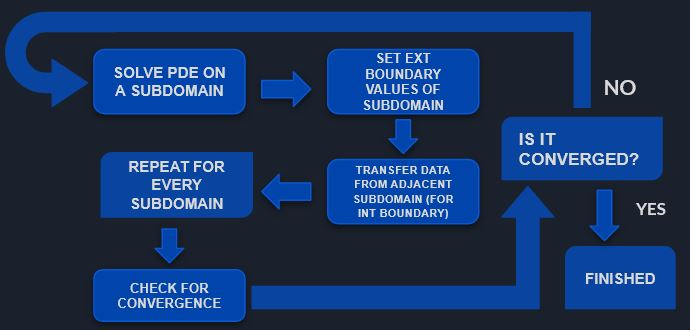
\includegraphics[width=\textwidth]{images/schwarz_basic_algo.JPG}
    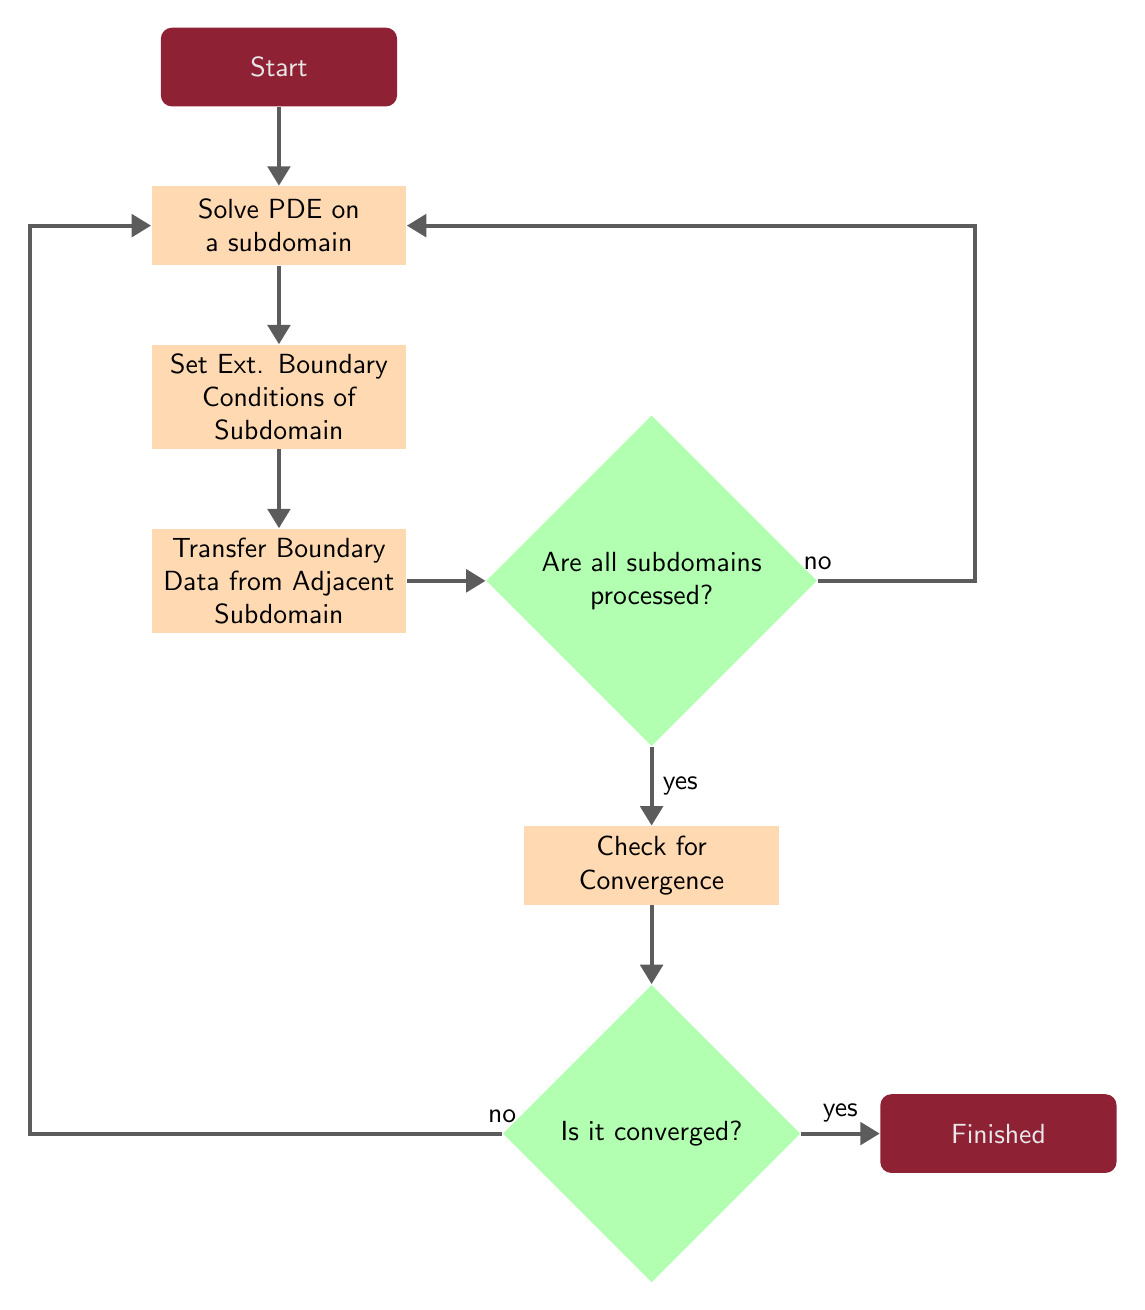
\begin{tikzpicture}


	\centering
	\sffamily

	%Creating the elements in the Schwarz Alternating Method
	\node (start) [startstop] {Start};
	%\node (domain_decomp) [process,below= of start] {Partition Comp. Domain into subdomains};
	\node (solve_pde) [process, below= of start] {Solve PDE on a subdomain};
	
	\node (solve_ext_BC) [process, below= of solve_pde] {Set Ext. Boundary Conditions of Subdomain};
	\node (transfer_data) [process, below = of solve_ext_BC] {Transfer Boundary Data from Adjacent Subdomain};
	\node (repeat_subdomain) [decision, right= of transfer_data] {Are all subdomains processed?};
	\node (check_conv) [process, below= of repeat_subdomain] {Check for Convergence};
	\node (domain_conv) [decision,below=of check_conv] {Is it converged?};
	\node (finished) [startstop, right= of domain_conv] {Finished};

	%Draw the arrows for the flowchart
	\draw [arrow_cap] (start) -- (solve_pde);
	%\draw [arrow_cap] (domain_decomp) -- (solve_pde);
	\draw [arrow_cap] (solve_pde) -- (solve_ext_BC);
	\draw [arrow_cap] (solve_ext_BC) -- (transfer_data);
	\draw [arrow_cap] (transfer_data) --(repeat_subdomain);
	\draw [arrow_cap] (repeat_subdomain) --  node[anchor=west] {yes} (check_conv);
	\draw [arrow_cap] (check_conv) --  (domain_conv);
	\draw [arrow_cap] (domain_conv) -- node[anchor=south] {yes} (finished);
	\draw [arrow_cap] (repeat_subdomain.east) |- node[anchor=south] {no} ++(2,0) |- (solve_pde.east);
	\draw [arrow_cap] (domain_conv.west) |- node[anchor=south] {no} ++(-6,0) |- (solve_pde.west);


    \end{tikzpicture}
    \caption{Schwarz Alternating Algorithm \cite{Tezaur2017}}
    \label{fig:schwarz_flowchart}
\end{figure} 

This domain decomposition method decomposes the whole computational domain into several subdomains where each subdomain has an overlapping region with each adjacent subdomain as a pre-processing step and the algorithm can be divided into two parts: the first part where it can be done asynchronously and the second part where each subdomain must do it synchronously.\\

These steps can be done by each subdomain asynchronously with respect to the other subdomains:

\begin{enumerate}
    \item Solve the partial differential equation on a subdomain
    \item Set the external boundary values of the subdomain (not including the inner boundaries as a consequence of partitioning the computational domain)
    
\noindent
After the first two steps, each subdomain must wait for their adjacent subdomain to finish before continuing the algorithm. The next half of the algorithm must be done synchronously because it requires the data transfer between the adjacent subdomains.

    \item Transfer the data from the adjacent subdomain/s to the inner boundary of the subdomain
    \item Check for convergence of each subdomain
\end{enumerate}

In the second part, each subdomain must finish the first part so that the data that will be transferred to the inner boundaries of each subdomain will be the updated value that has been computed in the first part. The importance of the overlapping region of this algorithm is for the convergence of the numerical solution. The convergence is validated by comparing the values in the overlapping regions of each subdomain such that they satisfy the condition shown below. If the convergence is achieved, the algorithm will proceed to post-processing, otherwise the algorithm will start to step 1 in the first half of the algorithm.

\begin{align}
    error \leq \epsilon_{tol}
    \label{eq:converge_cond}
\end{align}

A more in-depth description of the convergence method used in this project will be done in the implementation part.The $error$ is the error function that will be used to calculate the difference in values between overlapping regions while the $\epsilon_{tol}$ is the error tolerance that the algorithm uses to determine if the solution has converged. The important point in this part is that the Schwarz Alternating Method can validate whether each subdomain converges to one solution using the overlapping region/s in each subdomain.

\cleardoublepage

\chapter{Related Work\label{cha:RRW}}

% A review of previous work and other materials related to the project
% shall be written here. Make sure you do proper citations of original
% materials taken from various sources. For example, if this sentence
% is taken from reference \#1 in my bibliography, it should be referenced
% just like this {[}1{]}. Avoid copying sources word for word. Always
% paraphrase. \textquotedblleft If it cannot be avoided, enclose the
% cited material in double quotes just like this\textquotedblright{}
% {[}2{]}. If this whole paragraph was taken from two different sources,
% then the citations may be written this way {[}3{]}, {[}4{]}. 


\section{Finite-Difference Time Domain} \label{sec:FDTD}

The earliest known work related to numerically solving for partial difference equations was published in 1928 \cite{Courant1928}. Since then up until the 1960's, there only one literature that is related to time-dependent finite difference methods \cite{Taflove2005}. In 1966, Kane Yee \cite{Yee1966} applied finite-difference methods in solving for Maxwell's curl equations. The concept of staggering the electric and magnetic fields across space and time in a grid was also introduced in this work. The term ``Finite Difference Time Domain" was coined by Taflove in 1980 \cite{Taflove1980}. Since then, the Finite Difference Time Domain is used in scientific and engineering applications dealing with electromagnetic wave interactions. Its most prominent use is in the field of wireless communications, but other fields of study such as biomedicine and quantum mechanics have used FDTD as well \cite{Taflove2005}. Although the study and application of FDTD has been around for quite some time, research on the subject still continue based on recent studies \cite{Huang2020, Thomson2020, Algarni2020}. 


\subsection{Properties of the FDTD Method and Comparisons to Other Methods}\label{FDTDproperties}

 As mentioned in Chapter \ref{sec:bg}, there are several other  ways to numerically compute partial differential equations. This subsection will show some comparisons between FDTD and the aforementioned methods. This subsection will also shed some light on why FDTD is the most appropriate method for this study. \\

\noindent \textbf{Finite Element Method}\\

The finite element method is a widely used numerical method for solving PDEs in \textit{space} variables --- unlike FDTD which handles variables in space \textit{and} time. Similar to FDTD, it divides a problem into smaller parts called finite elements. These finite elements are made by constructing a 3D mesh of the object being modelled. These meshes can be of different shapes \cite{Logan2012}, which are in contrast to the usual cubic shapes of the FDTD subdomains (Yee Cells). 

When compared to FDTD, FEM can handle more complex geometries, since the meshes can be configured in different ways other than a cube \cite{Logan2012}. However, this leads to computational complexity. This is where FDTD has an advantage --- it is easier to implement. Also, FEM was initially developed for structural analysis \cite{Logan2012}, while FDTD was formulated for the purpose of numerically computing Maxwell's equations \cite{Yee1966}. \\

\noindent \textbf{Method of Moments}\\ 

The Method of Moments (MoM) uses the integral form of Maxwell's Equations instead of their differential forms \cite{Arvas2012} \cite{Costabel}. Like the Finite Element Method, it also constructs meshes on the surface of the model. However, unlike both FDTD and FEM, MoM operates only on the boundaries of the computational domain rather than the entire space. 

When compared to the two other methods, MoM is more efficient when the area-to-volume ratio is small. However, it becomes more computationally expensive as the complexity increases. Matrix sizes also increase with complexity \cite{Katsikadelis2002}.\\ 

\noindent \textbf{More Properties of FDTD}\\
Among the properties mentioned above, here are some more properties of FDTD according to Taflove \cite{Taflove2005}:

\begin{enumerate}
    \item It is intuitive and easy to implement 
    \item It is accurate and robust 
    \item It is a time-domain technique --- it can cover a wide range of frequency responses using a single simulation
    % \item The method itself allows for animation of the results for a more intuitive understanding of what happened in the simulation
    % \item It computes for the $\mathbf{E}$ and $\mathbf{H}$ fields directly --- no need to convert from one entity to another
    \item It does not require matrix inversion
    \item It efficiently scales well with parallel CPUs
    
\end{enumerate}

The properties mentioned above were the main driving force for several researches. Studies have used the FDTD method for its simplicity \cite{Ahmad2016, Liu2011, Kim2016}. The efficiency of FDTD in solving for Maxwell's equations was a key feature for one study \cite{Ahmad2016}. Another study mentioned that they chose FDTD for its wide coverage of frequencies \cite{Liu2011}. In this other study, they mentioned that they used FDTD because it does need matrix inversion \cite{Kim2016}. 

The project is an exploration of combining an electromagnetic wave simulation method with Schwarz Decomposition Method, which would verify if the data between two subdomains are accurate with each other. In order to maximize the chance of success, a suitable method must be chosen. Using the above properties, especially the simpleness, easiness to implement, and accuracy, FDTD is an excellent choice for this project. 

\subsection{Implementations of FDTD}

This subsection focuses on how studies implement FDTD. For this document, there will be two classes of implementations. First is the number of FDTD dimensions, and the second is how the FDTD method is combined with other methods. \\

\noindent \textbf{Number of FDTD Dimensions}

The FDTD method was originally formulated to solve for Maxwell's equations. Since Maxwell's equations describe quantities that are in three spatial dimensions, FDTD also has to do operations along the three dimensions. However, due to the staggered nature of the fields in the Yee cell, the FDTD method can be reduced to 2D or 1D \cite{Yee1966}, depending on the need of the user. 

% liu - 2D, Kim - 2D, Aono - 3D, Namiki - 2D, Garcia - 3D 
% In the researches found under FDTD, most of them were either 3D or 2D \cite{Liu2011}, \cite{Kim2016}, \cite{Aono2010}, \cite{Namiki1999}, \cite{Garcia2006}.

In the researches found under FDTD, most of them were either 3D \cite{Liu2011, Aono2010, Garcia2006} or 2D \cite{Namiki1999, Kim2016}. Only one study was found to incorporate 1D FDTD \cite{Ahmad2016}. However, since this project aims to combine FDTD with the Schwarz method, it would be best to start with simple, one-dimensional models. Also, this 1D setup can be scaled up to 2D and 3D should it prove to be successful. Implementing 1D FDTD is easy since references for this are readily available \cite{Houle2019, Rumpf082014, Taflove2005, Elsherbeni2015}.\\

\noindent \textbf{Configuration of Computational Domain} 
% (non-uniform cell size vs non-uniform computational domain)

FDTD operates on cells within its computational space. These cells can either be equally divided according to the size of the computational domain or be non-uniformly divided based on the complexity of whatever model is in the computational space. The former is the more basic way of implementing FDTD, and many studies still use this. The latter, however can be used to improve the performance and efficiency of the traditional FDTD implementation. 

Many of the structures being modelled nowadays are not uniform --- some of their parts might be more complex than other parts. By making the cells smaller at the more complex parts, the accuracy of the modelled EM phenomenon is increased. At the same time, less computational resources are allotted to the larger cells located along the less complex parts of the model. Studies have shown the improvements in computation time when using non-uniform grids. A study \cite{Song2018} showed that using non-uniform grid greatly decreases the computation time, thus improving efficiency. In another study \cite{Feng2021}, a modified FDTD algorithm that uses non-uniform grids was compared to the conventional FDTD implementation. The study noted that the computational efficiency of the former was superior to the conventional method. 


Another class of FDTD configuration is the non-uniform computational domain. In all of the previous works mentioned, none of them specified whether they did the study in a serial or in a parallel-configured computer. However, in one study \cite{Catarinucci2005}, a parallelized FDTD method in conjunction with a variable domain size was used. When compared to the previous computational domain configuration, the domain size per CPU core is non-uniform rather than cell sizes within a domain. This gives off an opportunity to assign more complex parts of the simulation to more powerful CPU cores. 

The aim of this project is more of a proof of concept -- that FDTD and Schwarz can be combined. Thus, the focus will be on trying to make them work together first. Computational efficiency of the devised method will only be secondary. Also, the project will deal only with one dimension. The need to vary the cell or computational domain size is unnecessary since the efficiency gains will not be seen with such a simple model. Thus, the uniform grid configuration is more fitting to be used in this project. \\

\noindent \textbf{FDTD in Conjunction with other methods}

Several studies have used the FDTD method alongside other techniques in order to optimize its performance. In one study \cite{Ahmad2016}, they used a Laplace Transform method to simplify the conductivity of their model. Other studies used different methods to improve the performance of their simulations. The moving window method was used in another study \cite{Liu2011} to reduce the computational resource usage of their simulation, while another study \cite{Kim2016} used topology optimisation for the same reason. Other methods were also presented by one study \cite{Costa2007}, such as Alternate Direction Scheme, subgridding, and hybrid approaches to be used in conjuction with FDTD. Another class of FDTD optimisation is to perform it on a parallelized system. This will be further discussed in subsection \ref{subsec:parallel_fdtd_research}. 

Following the idea that FDTD can be used alongside other methods, it can be inferred that the Schwarz method can also be used along with FDTD. 


\subsection{Simulation Models in Other Works}

Due to the ubiquity of FDTD in the electromagnetic simulation space, an extensive amount of studies used it to model their objects. Examples of structures modelled using FDTD in other works are thin conducting sheets \cite{Abboud2008}, plasma sheath of a hypersonic vehicle \cite{Liu2011}, graphene sheets \cite{Ahmad2016}, \cite{Ramadan2017}, 3D photonic crystals \cite{Hanawa2007}, and transmission lines \cite{Luo2020}, among many others. 

For this project, complex structures such as those mentioned above will not be used. Two simple models will be used instead. The first model is a computational domain split into cells with varying refractive indices. The second model is called Bragg Grating. More information on these two models will be discussed in subsection  \ref{meth:simmodels}


\section{Parallel Computing} \label{sec:parallel computing}

Parallel computing can be divided into two types depending on how the memory is accessed: shared memory (SM) and distributed memory (DM) architectures \cite{Yu2009,Ciamulski2008,Ciamulski2007}. 
\begin{figure}[H]

    \centering
    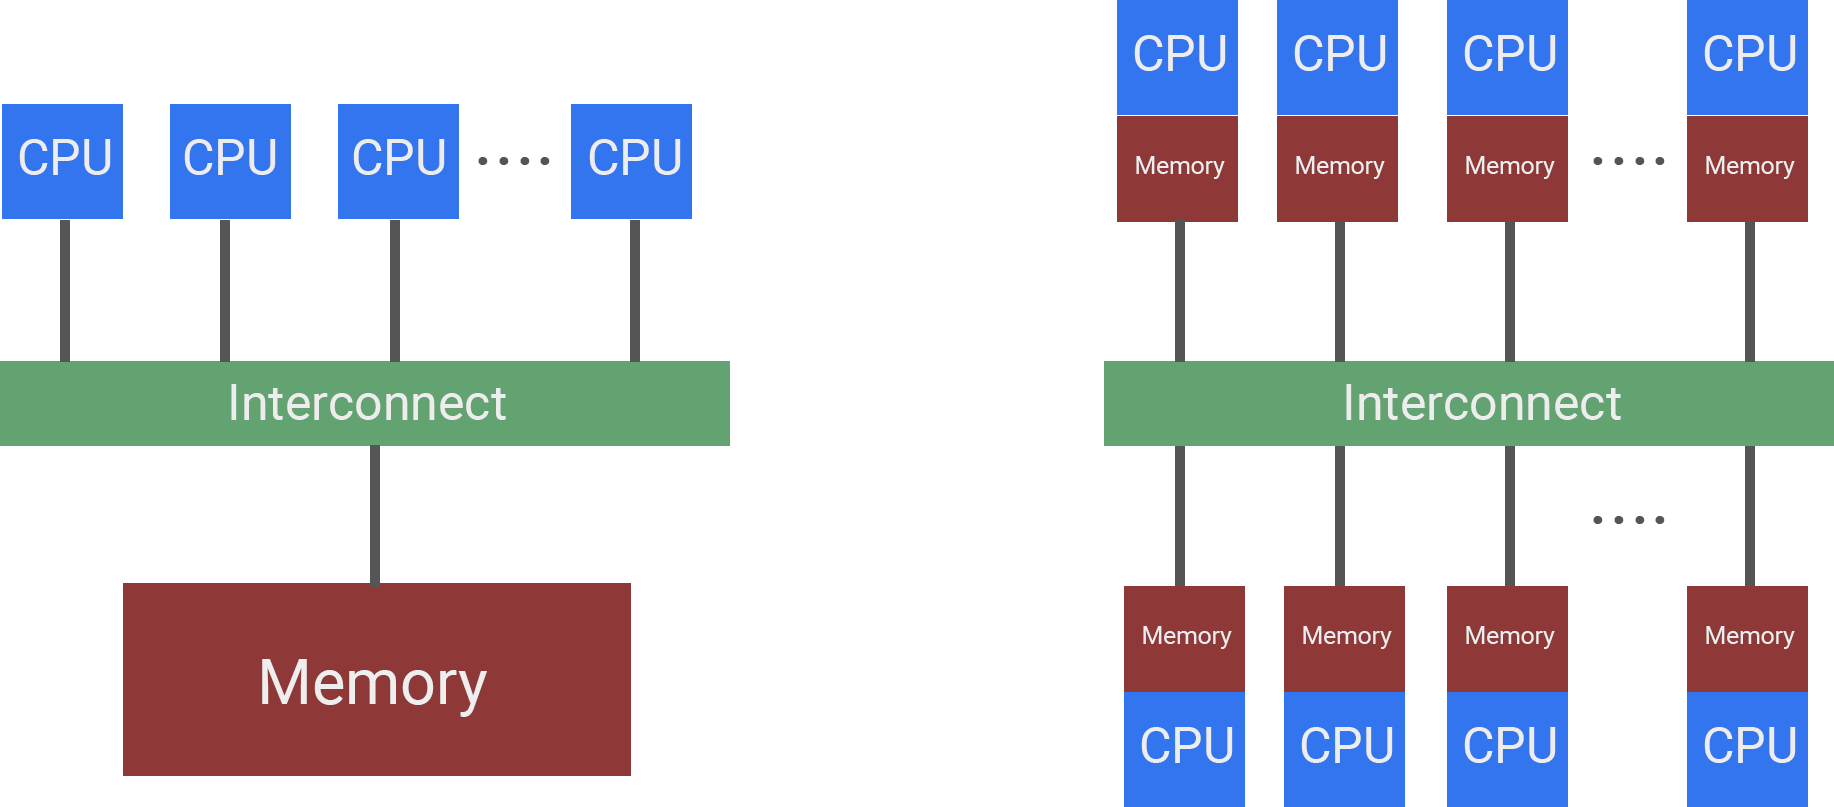
\includegraphics{images/SM_DM.png}
    \caption{Shared Memory (SM) (left) and Distributed Memory (DM) (right) architectures \cite{Busseuil2010}.}
    \label{fig:SMDM}
\end{figure}

Figure \ref{fig:SMDM} shows the two memory architectures used in parallel computing \cite{Busseuil2010}. SM architecture shows that each processor shares a memory block in the system while in DM, each processor has an independent memory block (memory is 'distributed' in each processor) that cannot be accessed by other processor. In the context of FDTD and computational domain, SM assigns each subdomain to a thread or process in a node while DM assigns each subdomain to a node in a cluster of computers \cite{Ciamulski2007}.

In order to facilitate communication between the different processors, message passing interface (MPI) protocol like MPICH or Intel MPI library is usually used (for DM) \cite{Luo2020, Zheng2016, Tan2018} and multi-threading libraries like OpenMP (for SM) \cite{Yu2009, Ciamulski2007, Yan2010}. MPI is a protocol generally used for communicating between independent processors in a network \cite{Karniadakis2003} while OpenMP can be thought of as MPI's equivalent in a multi-threading context (where there are multiple processes in a single CPU) that is popular in parallel computing research \cite{Yan2010}. There are also research \cite{Yan2010} that combines the use of MPI and OpenMP such that they have a hybrid memory architecture (SM and DM) such that the computational domain is divided into several nodes while each node has multiple threads that divide the subdomain into smaller subsubdomain.

In the context of this project, the primary focus will be on SM architecture that utilizes OpenMP because it is generally easier to implement given the small timeframe of the project and will be cheaper to implement because of the rising demand of cheap multi-core computers that has good single core performance \cite{Luo2020}. MPI and DM can still be considered for the project if time allows for it as the project progresses.

\subsection{Parallel FDTD Research}\label{subsec:parallel_fdtd_research}


Research in implementing FDTD in parallel configuration has already progress in the past decade. A common methodology in these studies \cite{Ramadan2017, Luo2020, Zheng2016, Yan2010, Lin2013, Yuan2011} shows that parallel FDTD algorithm use spatial division (or domain decomposition) of the computational domain is done and mapping each subdomain to either a thread (for SM type of parallel computing) or node (for DM type of parallel computing). This method of domain decomposition is intuitive because of how FDTD algorithm works that loops in the whole computational domain. Improvements on this methodology are done in \cite{Ramadan2017, Zhang2008, Li2009, Hanawa2007, Hanawa2005} by introducing overlaps in the subdomains (also referred as 'ghost cells') that serves as  storage of the boundary values of the adjacent subdomains for more efficient processing in each time step of the FDTD algorithm. Research in \cite{Yu2005} also shows a different method of setting the computational domain by using a non-uniform cell size such that smaller cell size is present in parts of the domain which has intricate/complex designs while larger cell size has simpler designs in the domain to increase the efficiency and minimize load problems in the computational domain.

 Another technique that is implemented in recent research is dividing the computational domain in only one direction to minimize the data communication overhead between adjacent subdomains \cite{Ramadan2017,  Yan2010, Zhang2008, Yu2005}. This minimizes the amount of data transfer between each subdomains since fewer artificial boundaries between subdomains are created. Other researches include \cite{Dong2005} that uses a different data structure (compressed octree) to alleviate load balancing problems in the computational domain brought about by complex geometries of the simulation models. Although these method are considered to be  a parallel process, the data transfer between adjacent subdomain is still a synchronous event that needs to be done by each subdomain. This may result in some subdomain `waiting' for all of the subdomain to be done processing before initiating the data transfer of the adjacent subdomains.


Data transfer between adjacent subdomains is evident across different methodologies \cite{Ramadan2017, Luo2020, Zheng2016, Lin2013, Yuan2011, Li2009, Yu2005, Hanawa2007} by using a master node/thread that synchronizes every subdomain's work in each iteration \cite{Ciamulski2008}. Improvements on minimizing the data communication overhead are also done in \cite{Yuan2011} by using a separate unit for communicating between adjacent subdomains and using a different communication protocol (Scalable Coherent Boundary Protocol or SCI) than the traditional MPI that results in 40\% increase in speedup than the common method.

%EDIT TO FOCUS ON ADVANTAGE OF USING PARALLEL COMPUTIING

Since most researches in parallel FDTD uses DM architecture, they have different procesors as well as memory blocks used in each node/subdomain. These nodes might have small discrepancies in how they process the data as well as the amount of noise introduced while processing the data that might cause cascading errors in the results. Utilizing Schwarz Algorithm (as discussed in chapter \ref{cha:Schwarz}) might help in minimizing errors that appear (as a validation method for the results) so that the system is reliable and accurate since most research in parallel FDTD do not check for the convergence of each subdomain. Also, taking advantage of consumer grade multi-core computers in parallel computing is a good compromise in performance and cost when compared to using supercomputers or clusters of high performance computers.


\section{Schwarz Method}

The Schwarz alternating method was first proposed in 1870, but is still a popular topic of study up to the present. It is a method for solving Laplace PDEs on irregular domains. It's main idea is to solve for an irregularly shaped domain using its parts that are regularly-shaped \cite{Tezaur2017}. 

Several studies \cite{Gnilenko2017, KhattriDDM, Li2020} have used  Schwarz method in conjunction with other numerical methods, but these studies do not deal with electromagnetic problems or FDTD. There has not been any literature on a combination of the FDTD and Schwarz methods as far as the proponents' knowledge goes. However, there are studies which solved electromagnetic problems using the Schwarz method in conjunction with other methods. In \cite{Spiteri2003}, a convection-diffusion problem was solved using parallel iterative methods. In \cite{Gnatyuk2015}, an optimal iteration was developed to extend the application range of the Schwarz method. In \cite{Gnilenko2017}, the Schwarz method was modified to use partial overlapping regions to solve for a boundary-value problem. The studies presented above show that Schwarz method can be modified and be used in conjunction with other computing techniques. This implies the possibility of using the Schwarz and FDTD method together. 

This project aims to combine Schwarz method with the FDTD method in a parallel computing environment. Section \ref{sec:parallel computing} provides some studies that already implemented FDTD in parallel. However, none of them were able to show whether the exchange of information between the sub-domains are accurate. As stated previously, it may be possible to use Schwarz in conjunction with the FDTD method. If that is the case, then it can be an improvement to the current parallel FDTD studies. 


\section{Cloud Computing}


\subsection{Infrastructure as a Service}

Infrastructure as a Service (IaaS) is a type of cloud computing service model  that are used when the cloud service providers will provide the memory, storage, computing resources and network while the customer will provide the necessary operating system and software necessary for their needs \cite{Mell2011}. This service allows for the customer the ``lowest level of control of the resources in the cloud" \cite{IBM2019}. In essence, this is basically a virtual machine in the cloud where the user can set their own computational needs and install their custom software. This service model is beneficial to parallel computing as it can reduce the cost of acquiring hardware and maintenance while it is being used

Popular IaaS from different service providers include: Amazon's Elastic Compute Cloud (EC2), Google Cloud Compute Engine, and Microsoft Azure Virtual Machines. These services have similar features that offer pre-installed virtual machine instances or installing custom images that contain necessary software and configuration for the user's needs and duplicating an instance of a newly created VM can also be done \cite{EC22021, ComputeEngine, AzureVM}. These features are advantageous in creating a cluster of nodes in the cloud since it will be cost-effective and easy to creating a cluster of similar nodes by using the different cloud platforms.

Although commercial cloud services are easier to use and popular in research, open source cloud frameworks such as SciCloud and Hadoop are also being developed as a way to creating a private cloud service in universities for efficient use of computational resources \cite{Srirama2010}.

\subsection{FDTD Cloud Computing Research}\label{subsec:cloud_fdtd_research}

As discussed in section \ref{subsec:parallel_fdtd_research}, many researches are done on parallel computing and some of them have already explored the idea of implementing these algorithms in the cloud \cite{Lin2013, Gope2011, McDonald2013, Tan2018}. 

Most of them \cite{McDonald2013, Tan2018, Gope2011} uses Amazon EC2 while \cite{Lin2013} uses cloud computing framework like SciCloud and Hadoop. In \cite{McDonald2013}, identical setups (FDTD code, MPI libraries, and configuration) are done on a local cluster of computers and on Amazon EC2 instance. The results of a series of tests shows that there are no significant drawbacks on using a cloud setup in comparison on a local setup. In another study \cite{Tan2018}, the use of cloud computing in solving EM problems using parallel FDTD is not worse than using a supercomputer. The results of these studies show that cloud computing does not provide any significant advantage in the speed and accuracy of the algorithm since their results are similar to local setups. 


In these studies, the implementation of the algorithm in the cloud is similar to how the algorithm is implemented on-site so it seems that the main purpose of utilizing cloud computing in these studies is to ascertain the viability of cloud computing for research. The ability of cloud computing to assign resources depending on the demand also helps balance the computational power and cost since as most research in parallel FDTD show, efficiency usually drops as the number of nodes (processors) increase in a simulation run. So, it is evident that parallel computing and cloud computing is an effective and viable solution for cost-effective computing resources as the studies shows positive results in using cloud resources.


\section{Synthesis}


% Several concepts were discussed in the above sections. Section \ref{sec:FDTD} provides some information on the FDTD method, and why it was chosen for this project. 

The works presented in each subsection greatly aided in the positioning of this project among the current studies in FDTD, Schwarz method, and parallel computing. They provided information on how and why the methods were used in the context of numerically solving for electromagnetic phenomena. With the help of the works mentioned, the proponents now have a foundation to which project objectives can be built upon. Other aspects of the project such as the scope and methodology can also be greatly influenced by these works. Combining all of the ideas from the different literatures, the proponents believe that this undergraduate project can help in alleviating the need of powerful hardware in solving electromagnetic problems.

% Combining all of the ideas from the works, the proponents believe that they can produce an undergraduate project which can contribute to the fields of FDTD, parallel computing, and the Schwarz method. 



\cleardoublepage{}

\chapter{Problem Statement and Objectives} \label{cha:ProbStatement}

%Insert introductory paragraph


\section{Problem Statement}

Students predominantly have no access to powerful computational devices when doing electromagnetic simulations. Such simulation jobs are difficult to do on low-end hardware due to their mathematical complexity, complex design, and scale. Electromagnetics usually involves partial differential equations, which needs to be computed numerically for computers to solve them. The Finite Difference Time-Domain algorithm is a popular numerical method used for EM simulation problems due to its simplicity and fast processing.



The gap between the lack of powerful hardware and the need for EM simulations can be narrowed by implementing an established FDTD algorithm in a parallel environment. This implementation is parallelized using domain decomposition via the Schwarz method. By implementing this method, workflows may run faster and can be more accessible while maintaining accuracy and reliability.

\section{Specific Objectives}
\begin{enumerate}
    \item Develop serial Finite Difference Time Domain code in 1D based on currently existing FDTD algorithms.
    \item Implement the developed 1D FDTD code in serial and parallel configuration using similar simulation parameters.
    \item Use Schwarz method to validate whether or not the data computed in the parallel configuration is accurate with respect to the serial configuration and the analytical solution.  
    \item Assess the speedup and efficiency of our developed code simulation results on the three configurations, then compare the results to the open-source FDTD code run on the same configurations. 
\end{enumerate}
\section{Scopes and Limitations}

This part discusses the scope and limitations of the project to properly set the boundaries of the research.

\subsection{FDTD}

For this project, only Ampere's Law and Faraday's Law of Induction will be focused on. The project's scope is only 1-dimensional plane wave propagation, and the last two Maxwell's equations are enough to model it. Ampere's Law and Faraday's Law of Induction shall be known as the Curl Equations for the rest of this document. 

A few assumptions for Maxwell's Equations are made for this project. These assumptions will simplify the calculations to be made, and are enough to satisfy the goal of this project. The assumptions are as follows \cite{Rumpf2014}: 

\begin{enumerate}
    \item There is no charges or current sources in the system.
    \item The materials used are linear, isotropic, and non-dispersive.
    \item Cell size ($\Delta z$) is uniform in each part of the computational domain.
\end{enumerate}

As a result of these assumptions, the Curl Equations will reduce to the following: 

\begin{equation}
    \nabla \times \mathbf{H} = \frac{\partial \mathbf{D}}{\partial t} \quad \text{and} \quad \nabla \times \mathbf{E} = -\frac{\partial \mathbf{B}}{\partial t}
\end{equation}

\subsection{Schwarz Alternating Method}

The assumptions for the Schwarz Alternating Method for this project is shown below:

\begin{enumerate}
    \item Length of overlapping region must be greater than 0 ($\Omega_i \cap \Omega_{i+1}$).
    \item Each subdomain must have an equal amount of cells.
    \item Convergence is checked after each cell in the computational domain is solved.
\end{enumerate}

The first assumption deals with the requirement of convergence \cite{Tezaur2017} for the algorithm since the overlapping region is used to check for convergence. The second assumption is related to the FDTD-Schwarz Algorithm since having a uniform size in each subdomain can simplify the implementation of the algorithm. Also, this assumption will prevent any load-balancing techniques to be done. The last assumption is also done to prevent the algorithm from going to the next iteration without ensuring that the current iteration has converged successfully.


\subsection{Configuration}

In this project's context, although the proposed solution is parallel computing in the cloud, the methodology (in chapter \ref{cha:Methodology}) ignores the cloud computing aspect since the steps that need to be done on-site and in the cloud setup are similar (as shown in subsection \ref{subsec:cloud_fdtd_research}). The only difference is on how the set up the virtual machines or local computers before installing the necessary software and configurations for the parallel FDTD algorithm.




\cleardoublepage{}

\chapter{Methodology\label{cha:Methodology}}
%Put introductory paragraph


\section{Design}\label{sec:design}

% \subsection{1D FDTD Algorithm (To be transferred to Chapter 2)}\label{subsec:fdtd_method}

% As discussed in Chapter \ref{cha:RRW}, FDTD is a finite-difference method used to solve Maxwell's equations numerically \cite{Houle2019}. In its simplest form, it can be used to calculate the electric and magnetic field in the simulation space separately. The scope for this project is to use a FDTD in one dimension, which is the simplest type of FDTD that can be used to show if the parallel configuration is better than serial configuration. The most basic algorithm of FDTD is the leapfrog method \cite{Rumpf2014} that alternates in solving for the electric and magnetic field in each Yee cell using the update equations \cite{Houle2019}. The update equations used in this project are the Ey/Hx form of the FDTD Update equation in 1D \cite{Rumpf082014} and this form is chosen arbitrarily since the other form Ex/Hy is similar to the Ey/Hx form. The difference is the convention of the directions of the electric and magnetic fields in the simulation space.


% \begin{align}
%     &\tilde{H_x}|^{k}_{t+\frac{\Delta t}{2}}\,=\,\tilde{H_x}|^{k}_{t-\frac{\Delta t}{2}}\,+\,(m_{H_x}|^k)(\frac{E_{y}|_{t}^{k+1}\,-\,E_{y}|_{t}^{k}}{\Delta z})\label{eq:updateH}\\
%     &E_{y}|^{k}_{t+\Delta t}\,=\,E_{y}|^{k}_{t}\,+\,(m_{E_y}|^k)(\frac{\tilde{H_x}|_{t+\frac{\Delta t}{2}}^{k}\,-\,\tilde{H_x}|_{t+\frac{\Delta t}{2}}^{k-1}}{\Delta z})\label{eq:updateE}\\
%     &m_{E_y}|^{k}\,=\,\frac{c_0 \Delta t}{\epsilon _{yy}|^{k}}\label{eq:update_coeffE}\\
%     &m_{H_x}|^{k}\,=\,\frac{c_0 \Delta t}{\mu _{xx}|^{k}}
%     \label{eq:update_coeffH}
% \end{align}

% The equation above shows the update equations and the update coefficients for both the electric and magnetic fields for the FDTD algorithm. There are two important points about the update equations that need to be discussed: their dependence on previous value and adjacent values. First, the first term in the update equation is the previous field value (for both electric and magnetic field) so, every value in the k-th position in space is dependent on the previous time step. Second, the dependence on adjacent cells, since the electric field has a term for the magnetic field in k-1 position, this means that the electric field is dependent on the adjacent magnetic field value while the magnetic field is dependent on the adjacent electric field value (because it has an electric field in k+1 position).

% The implication of these dependence in time and space is that when the algorithm is parallelized and the whole computational domain is partitioned, there must be some sort of data communication between the different subdomain such that the adjacent cells can be extracted from the adjacent subdomain as well as their values in the previous time step.

% \begin{figure}[H]
%     \centering
%     %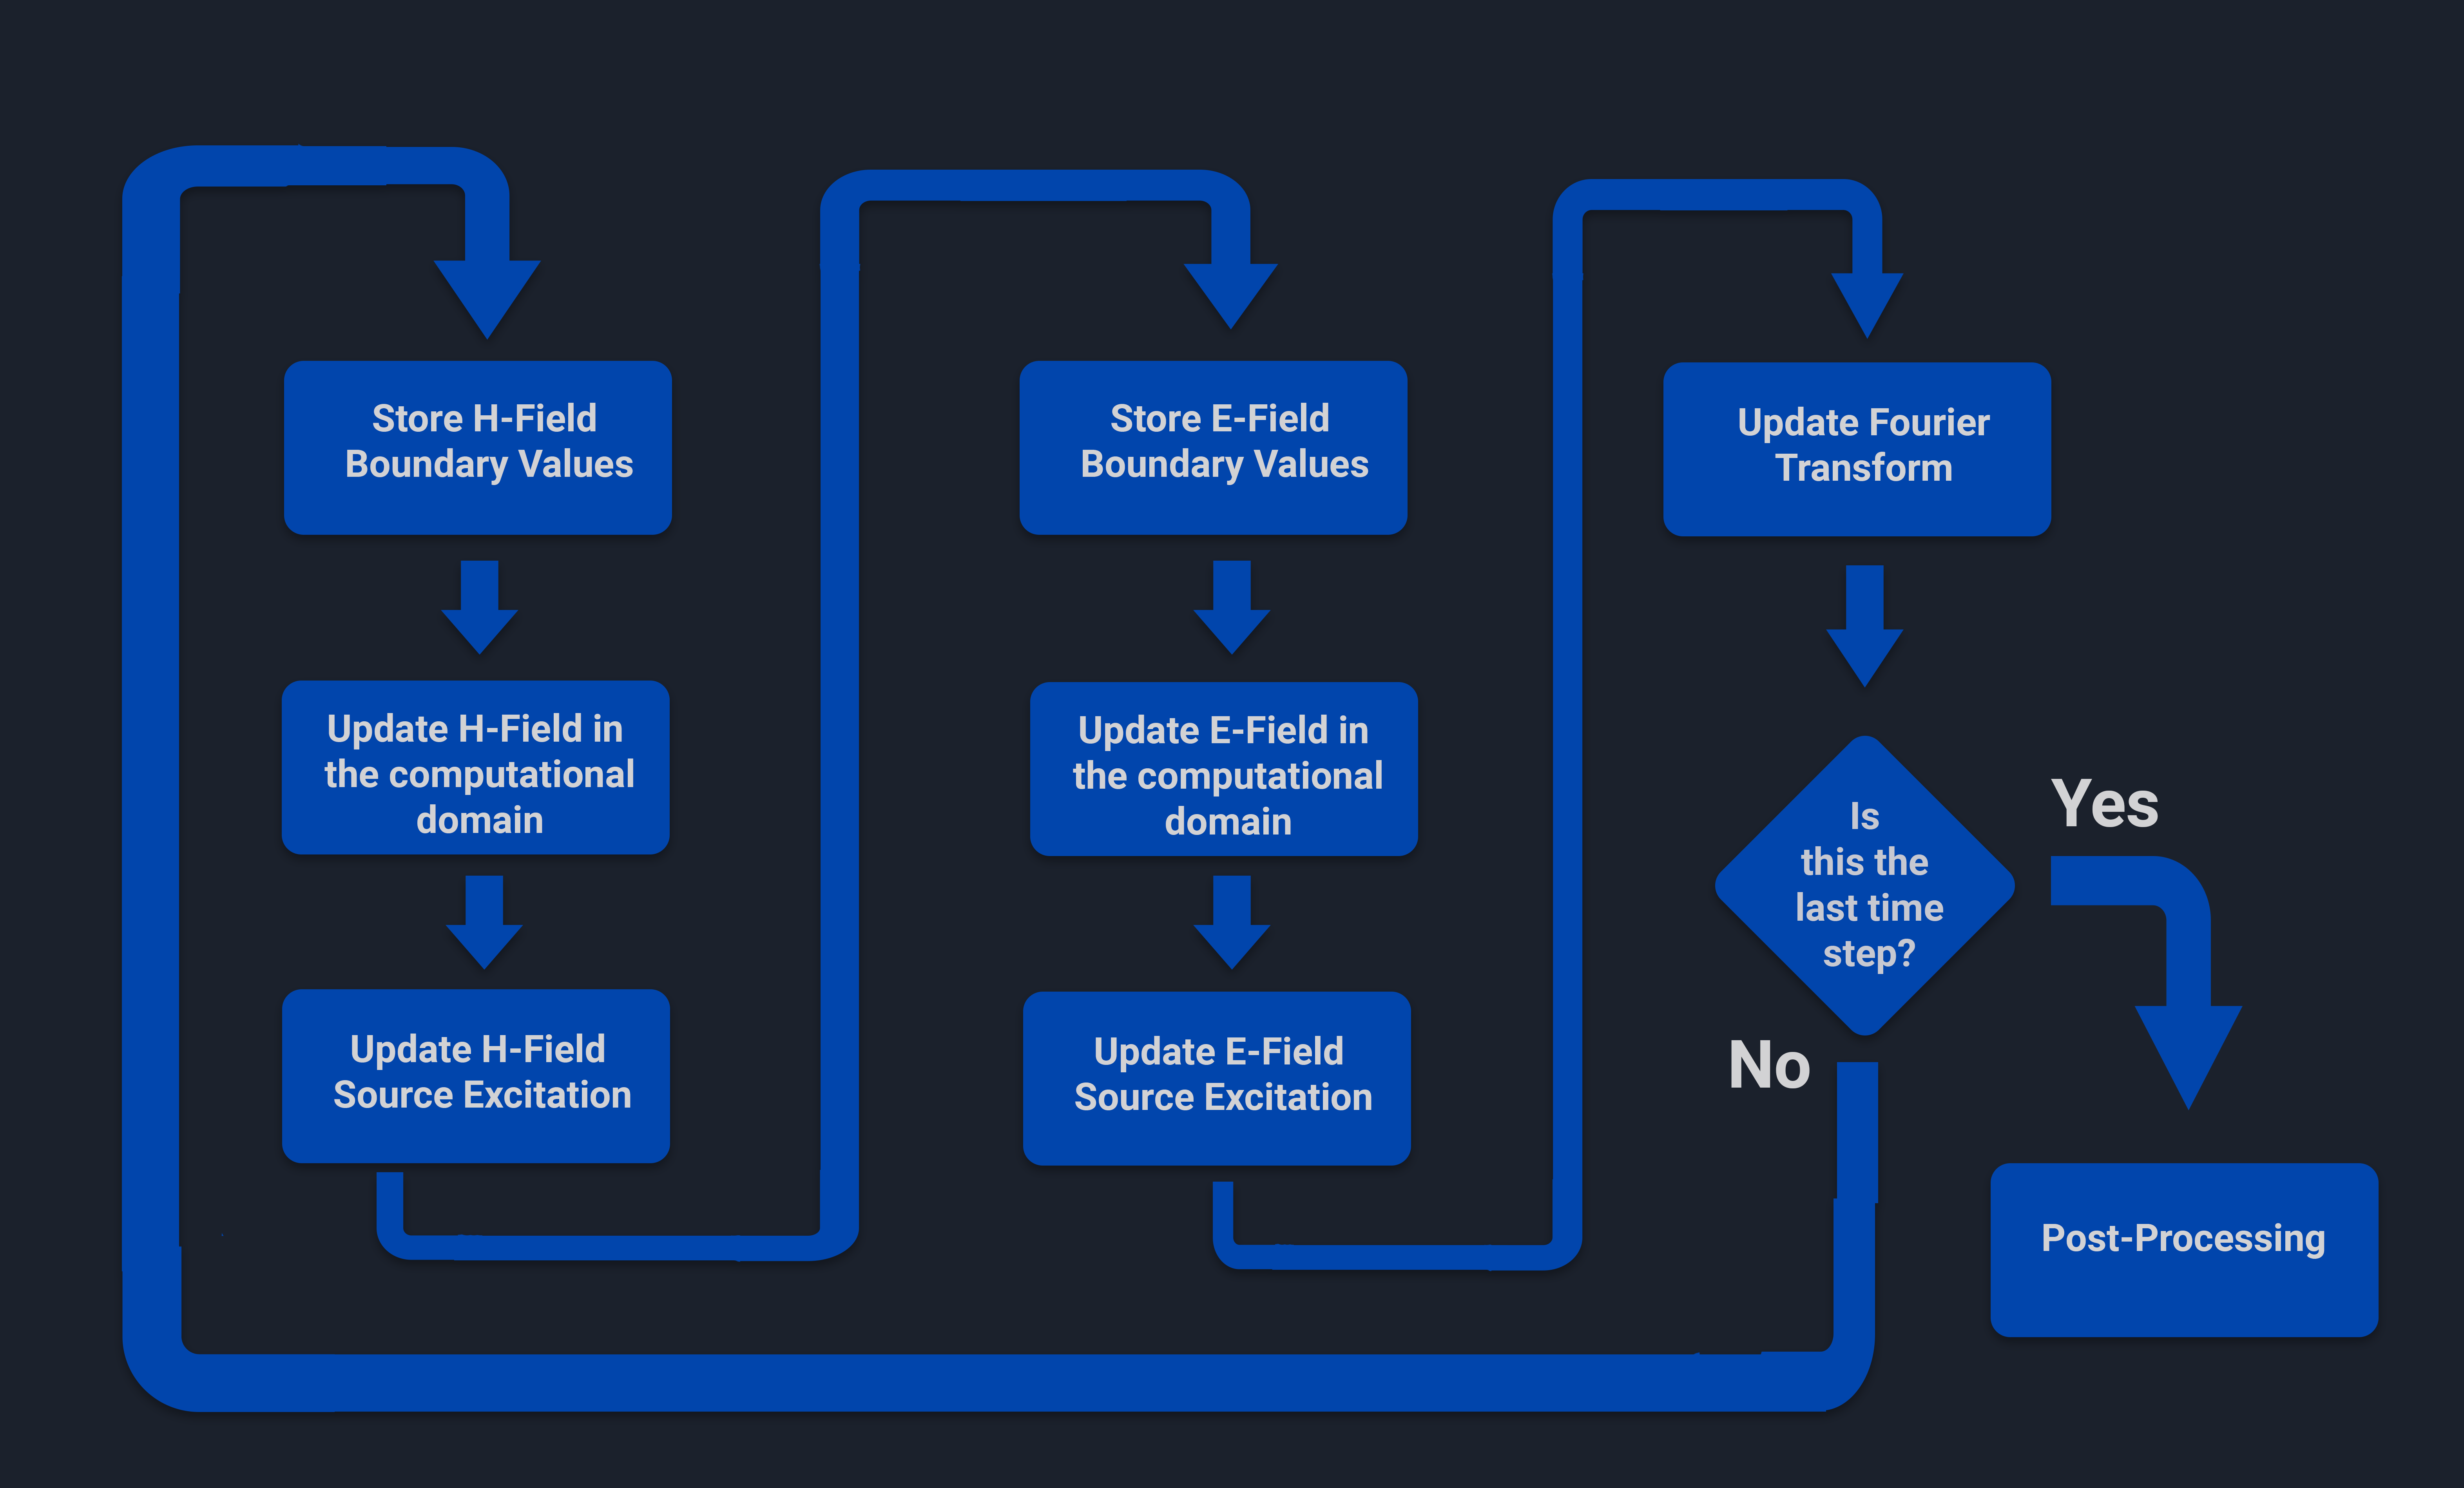
\includegraphics[width=\textwidth]{images/fdtdloop.png}
%     \resizebox{!}{\textheight}{
%     \begin{tikzpicture}
% 	\centering
% 	\sffamily
% 	%Creating the elements in the FDTD Flowchart
% 	\node (pre_process) [startstop] {Start};
% 	\node (store_Hboundary_terms) [process, below=of pre_process] {Store $\tilde{H}_x$ boundary terms};
% 	\node (update_H) [process, below= of store_Hboundary_terms] {Update $\tilde{H}_x$ in Computational Domain};
% 	\node (update_source_H) [process, below= of update_H] {Update $\tilde{H}_x$ source excitation};
% 	\node (store_Eboundary_terms) [process, below=of update_source_H] {Store $E_y$ boundary terms};
% 	\node (update_E) [process, below= of store_Eboundary_terms] {Update $E_y$ in Computational Domain};
% 	\node (update_source_E) [process, below= of update_E] {Update $E_y$ source excitation};
% 	\node (update_FFT) [process, below = of update_source_E] {Update FFT};
% 	\node (last_iter) [decision, below = of update_FFT] {Is it the last iteration?};
% 	\node (post_process) [startstop, below = of last_iter] {Finished};

% 	%Draw the arrows for the flowchart
% 	\draw [arrow_cap] (pre_process) -- (store_Hboundary_terms);
% 	\draw [arrow_cap] (store_Hboundary_terms) -- (update_H);
% 	\draw [arrow_cap] (update_H) -- (update_source_H);
% 	\draw [arrow_cap] (update_source_H) -- (store_Eboundary_terms);
% 	\draw [arrow_cap] (store_Eboundary_terms) -- (update_E);
% 	\draw [arrow_cap] (update_E) -- (update_source_E);
% 	\draw [arrow_cap] (update_source_E) -- (update_FFT);
% 	\draw [arrow_cap] (update_FFT) -- (last_iter);
% 	\draw [arrow_cap] (last_iter) -- node[anchor=east] {yes} (post_process);
% 	\draw [arrow_cap] (last_iter) --  node[anchor=north] {no, go to next iteration} ++(5.5,0) |- ++(0,18)   |- (store_Hboundary_terms.east);
	
%     \end{tikzpicture}
%     }
%     \caption{1D FDTD Algorithm}
%     \label{fig:fdtd_flowchart}
% \end{figure} 


% The flowchart shown in Fig \ref{fig:fdtd_flowchart} is the main algorithm of FDTD that computes for the field values in space and time. There are other steps like the pre-processing and post-processing that will be discussed in the implementation part of this chapter. In general, the FDTD algorithm has two main loops: the main loop that iterates through every time step, which will be referred here as the FDTD time loop and the inner loop that iterates through every cell in the computational domain, referred here as the FDTD space loop.

% First, the FDTD time loop is where the main steps of the algorithm are done. There are three main steps: 

% \begin{enumerate}
%     \item Updating the magnetic field value
%     \item Updating the electric field values
%     \item Updating the Fourier Transform and checking the stop condition
% \end{enumerate}

% The first and second steps are similar, the only difference is what field values are updated. This first two step can be referred to as FDTD space loop. The initial step in this part is to store the boundary values of magnetic or electric fields for the computation of the boundary condition in the next step. Next, to update the field values in the computational domain including the external boundary conditions of the domain, the FDTD space loop is involved since the iteration will be done through every cell in the computational domain. The update equation specified in \ref{eq:updateE} and \ref{eq:updateH} will be used to update each cell and after updating the cells in the whole computational domain, the algorithm will exit the FDTD space loop and proceed to the source excitation. 

% The injection of source excitation is done after the FDTD space loop where the source excitation (computed in the pre-processing stage) will be used by injecting, depending on the method of excitation into the specified injection point ($k_{inj}$). This will affect the field values since the field values have a dependence on the adjacent cells and so, the effect of the source excitation will be seen after the current iteration in the FDTD time loop is finished. The method on how the source excitation is injected into $k_{inj}$ and what types of sources will be used in the project will be discussed in the implementation part.


% After the storing of boundary values of the electric and magnetic fields, FDTD space loop for electric and magnetic fields, and the source excitation of the electric and magnetic field components, the last step in the FDTD time loop is the update of Fourier transform and checking of the stop condition. The  Fourier transform of each iteration in the FDTD time loop can be used to compute for the reflection and transmission coefficients for a specified frequency since FDTD is a time-based method, a single simulation run can include a wide range of frequencies \cite{Rumpf082014}. The equation used for calculating the reflection and transmission coefficients are shown below:

% \begin{align}
%     &R(f)\,=\,(\frac{FFT[E_{ref}(t)]}{FFT[E_{src}(t)]})^{2}\\
%     &T(f)\,=\,(\frac{FFT[E_{trn}(t)]}{FFT[E_{src}(t)]})^2\\
%     &C(f)\,=\,R(f)\,+\,T(f)
% \end{align}

% The reflected and transmitted fields are converted into the frequency domain by Fast Fourier Transform, and the fields are normalized with respect to the source excitation. The law of conservation of energy is also checked by getting the sum of the reflected and transmitted fields \cite{Rumpf082014}. This equation holds true in this situation because in the current FDTD model, the conductivity or the absorption loss after passing through a material is not taken into account so there should be no loss of energy because of the conductivity of the materials. The reflected and transmitted fields are measured at the first and last cells of the computational domain for the reflected and transmitted fields respectively. 

% The stop condition for the FDTD time loop is when the current iteration reaches the time specified in the pre-processing stage. If the current iteration reaches the last timestep, the FDTD time loop is finished and the algorithm will proceed to post-processing, otherwise, the algorithm continues to the next iteration of the FDTD time loop.


% \subsection{Schwarz Alternating Method}\label{subsec:schwarz}

% The Schwarz Alternating Method or Schwarz Multiplicative Method is a type of Domain Decomposition method under the overlapping domain kind \cite{Edelman2009} which as the name implies, uses the overlapping domain between the different subdomain to check the convergence of the whole computational domain/simulation space \cite{Dolean2021}. This particular method is the simplest form of overlapping domain type of domain decomposition that uses Dirichlet boundary conditions \cite{Maroudas2015} at the external boundaries of the computational domain. The basic algorithm of the method is shown below:

% %INSER SCHWARZ ALGO
% \begin{figure}[H]
%     \centering
%     %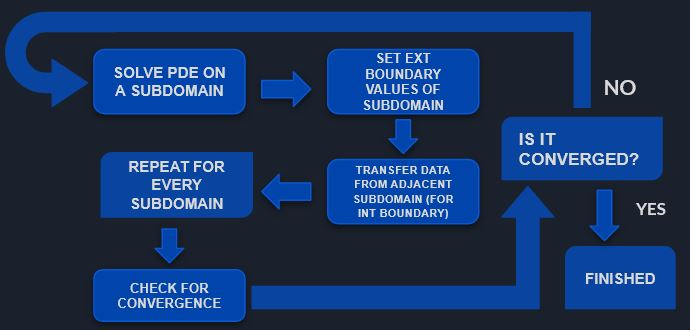
\includegraphics[width=\textwidth]{images/schwarz_basic_algo.JPG}
%     \begin{tikzpicture}


% 	\centering
% 	\sffamily

% 	%Creating the elements in the Schwarz Alternating Method
% 	\node (start) [startstop] {Start};
% 	%\node (domain_decomp) [process,below= of start] {Partition Comp. Domain into subdomains};
% 	\node (solve_pde) [process, below= of start] {Solve PDE on a subdomain};
	
% 	\node (solve_ext_BC) [process, below= of solve_pde] {Set Ext. Boundary Conditions of Subdomain};
% 	\node (transfer_data) [process, below = of solve_ext_BC] {Transfer Boundary Data from Adjacent Subdomain};
% 	\node (repeat_subdomain) [decision, right= of transfer_data] {Are all subdomains processed?};
% 	\node (check_conv) [process, below= of repeat_subdomain] {Check for Convergence};
% 	\node (domain_conv) [decision,below=of check_conv] {Is it converged?};
% 	\node (finished) [startstop, right= of domain_conv] {Finished};

% 	%Draw the arrows for the flowchart
% 	\draw [arrow_cap] (start) -- (solve_pde);
% 	%\draw [arrow_cap] (domain_decomp) -- (solve_pde);
% 	\draw [arrow_cap] (solve_pde) -- (solve_ext_BC);
% 	\draw [arrow_cap] (solve_ext_BC) -- (transfer_data);
% 	\draw [arrow_cap] (transfer_data) --(repeat_subdomain);
% 	\draw [arrow_cap] (repeat_subdomain) --  node[anchor=west] {yes} (check_conv);
% 	\draw [arrow_cap] (check_conv) --  (domain_conv);
% 	\draw [arrow_cap] (domain_conv) -- node[anchor=south] {yes} (finished);
% 	\draw [arrow_cap] (repeat_subdomain.east) |- node[anchor=south] {no} ++(2,0) |- (solve_pde.east);
% 	\draw [arrow_cap] (domain_conv.west) |- node[anchor=south] {no} ++(-6,0) |- (solve_pde.west);


%     \end{tikzpicture}
%     \caption{Schwarz Alternating Algorithm}
%     \label{fig:schwarz_flowchart}
% \end{figure} 





% This domain decomposition method decomposes the whole computational domain into several subdomain where each subdomain has an overlapping region with each adjacent subdomain as a pre-processing step and the algorithm can be divided into two parts: the first part where it can be done asynchronously and the second part where each subdomain must do it synchronously:

% These steps can be done by each subdomain asynchronously with respect to the other subdomains:

% \begin{enumerate}
%     \item Solve the partial differential equation on a subdomain
%     \item Set the external boundary values of the subdomain (not including the inner boundaries as a consequence of partitioning the computational domain)
    
% \noindent
% After the first two steps, each subdomain must wait for their adjacent subdomain to finish before continuing the algorithm. The next half of the algorithm must be done synchronously because it requires the data transfer between the adjacent subdomains.

%     \item Transfer the data from the adjacent subdomain/s to the inner boundary of the subdomain
%     \item Check for convergence of each subdomain
% \end{enumerate}

% In the second part, each subdomain must finish the first part so that the data that will be transferred to the inner boundaries of each subdomain will be the updated value that has been computed in the first part. The importance of the overlapping region of this algorithm is for the convergence of the numerical solution. The convergence is validated by comparing the values in the overlapping regions of each subdomain such that they satisfy the condition shown below. If the convergence is achieved, the algorithm will proceed to post-processing, otherwise the algorithm will start to step 1 in the first half of the algorithm.

% \begin{align}
%     error \leq \epsilon_{tol}
%     \label{eq:converge_cond}
% \end{align}

% A more in-depth description of the convergence method used in this project will be done in the implementation part.The error is the error function that will be used to calculate the difference in values between overlapping regions while the $\epsilon_{tol}$ is the error tolerance that the algorithm uses to determine if the solution has converged. The important point in this part is that the Schwarz Alternating Method can validate whether each subdomain converges to one solution using the overlapping region/s in each subdomain.


\subsection{Parallel FDTD via Schwarz Alternating Method}\label{subsec:fdtd_schwarz_disc}

The FDTD algorithm and Schwarz Alternating Method will be combined to create an FDTD algorithm that can be used in a parallel configuration. The purpose of including the Schwarz Alternating Method is to have a consistent way of validating the convergence of the solution when the computational domain is partitioned into subdomains. Most of the research \cite{Ramadan2017, Ciamulski2008, Luo2020, Li2009, Gedney1994, McDonald2013} done does not check the convergence of the solution, but simply partition the computational domain and facilitate the data exchange between adjacent subdomains due to the dependence of the equations \ref{eq:updateE} and \ref{eq:updateH} to the adjacent cells. The flowchart for the combined algorithm of FDTD and Schwarz Alternating Method is shown below:


\begin{figure}[H]
    \centering
    %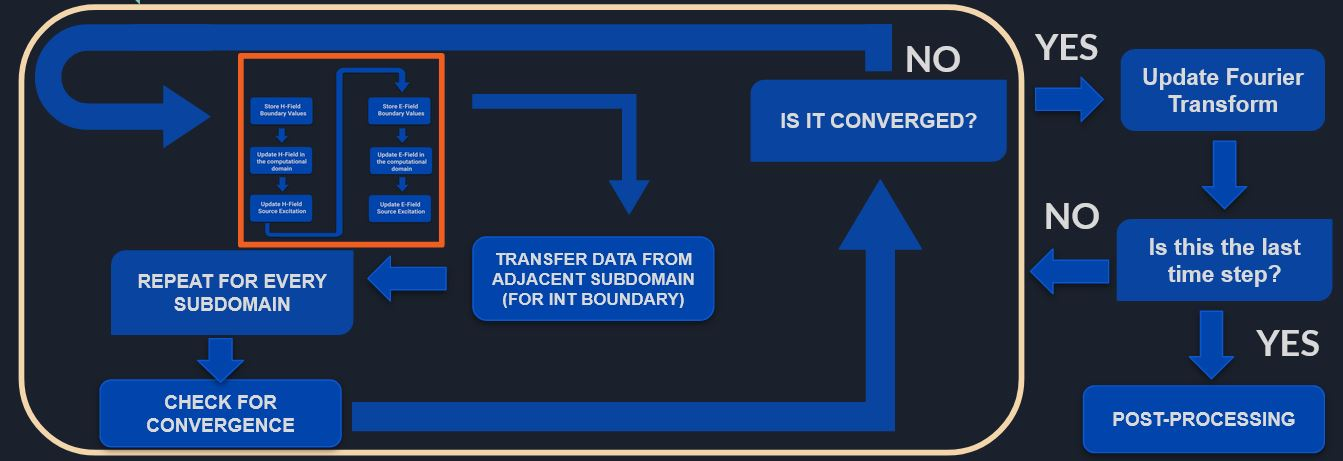
\includegraphics[width=\textwidth]{images/combined algo.JPG}
    \resizebox{!}{\textheight}{
    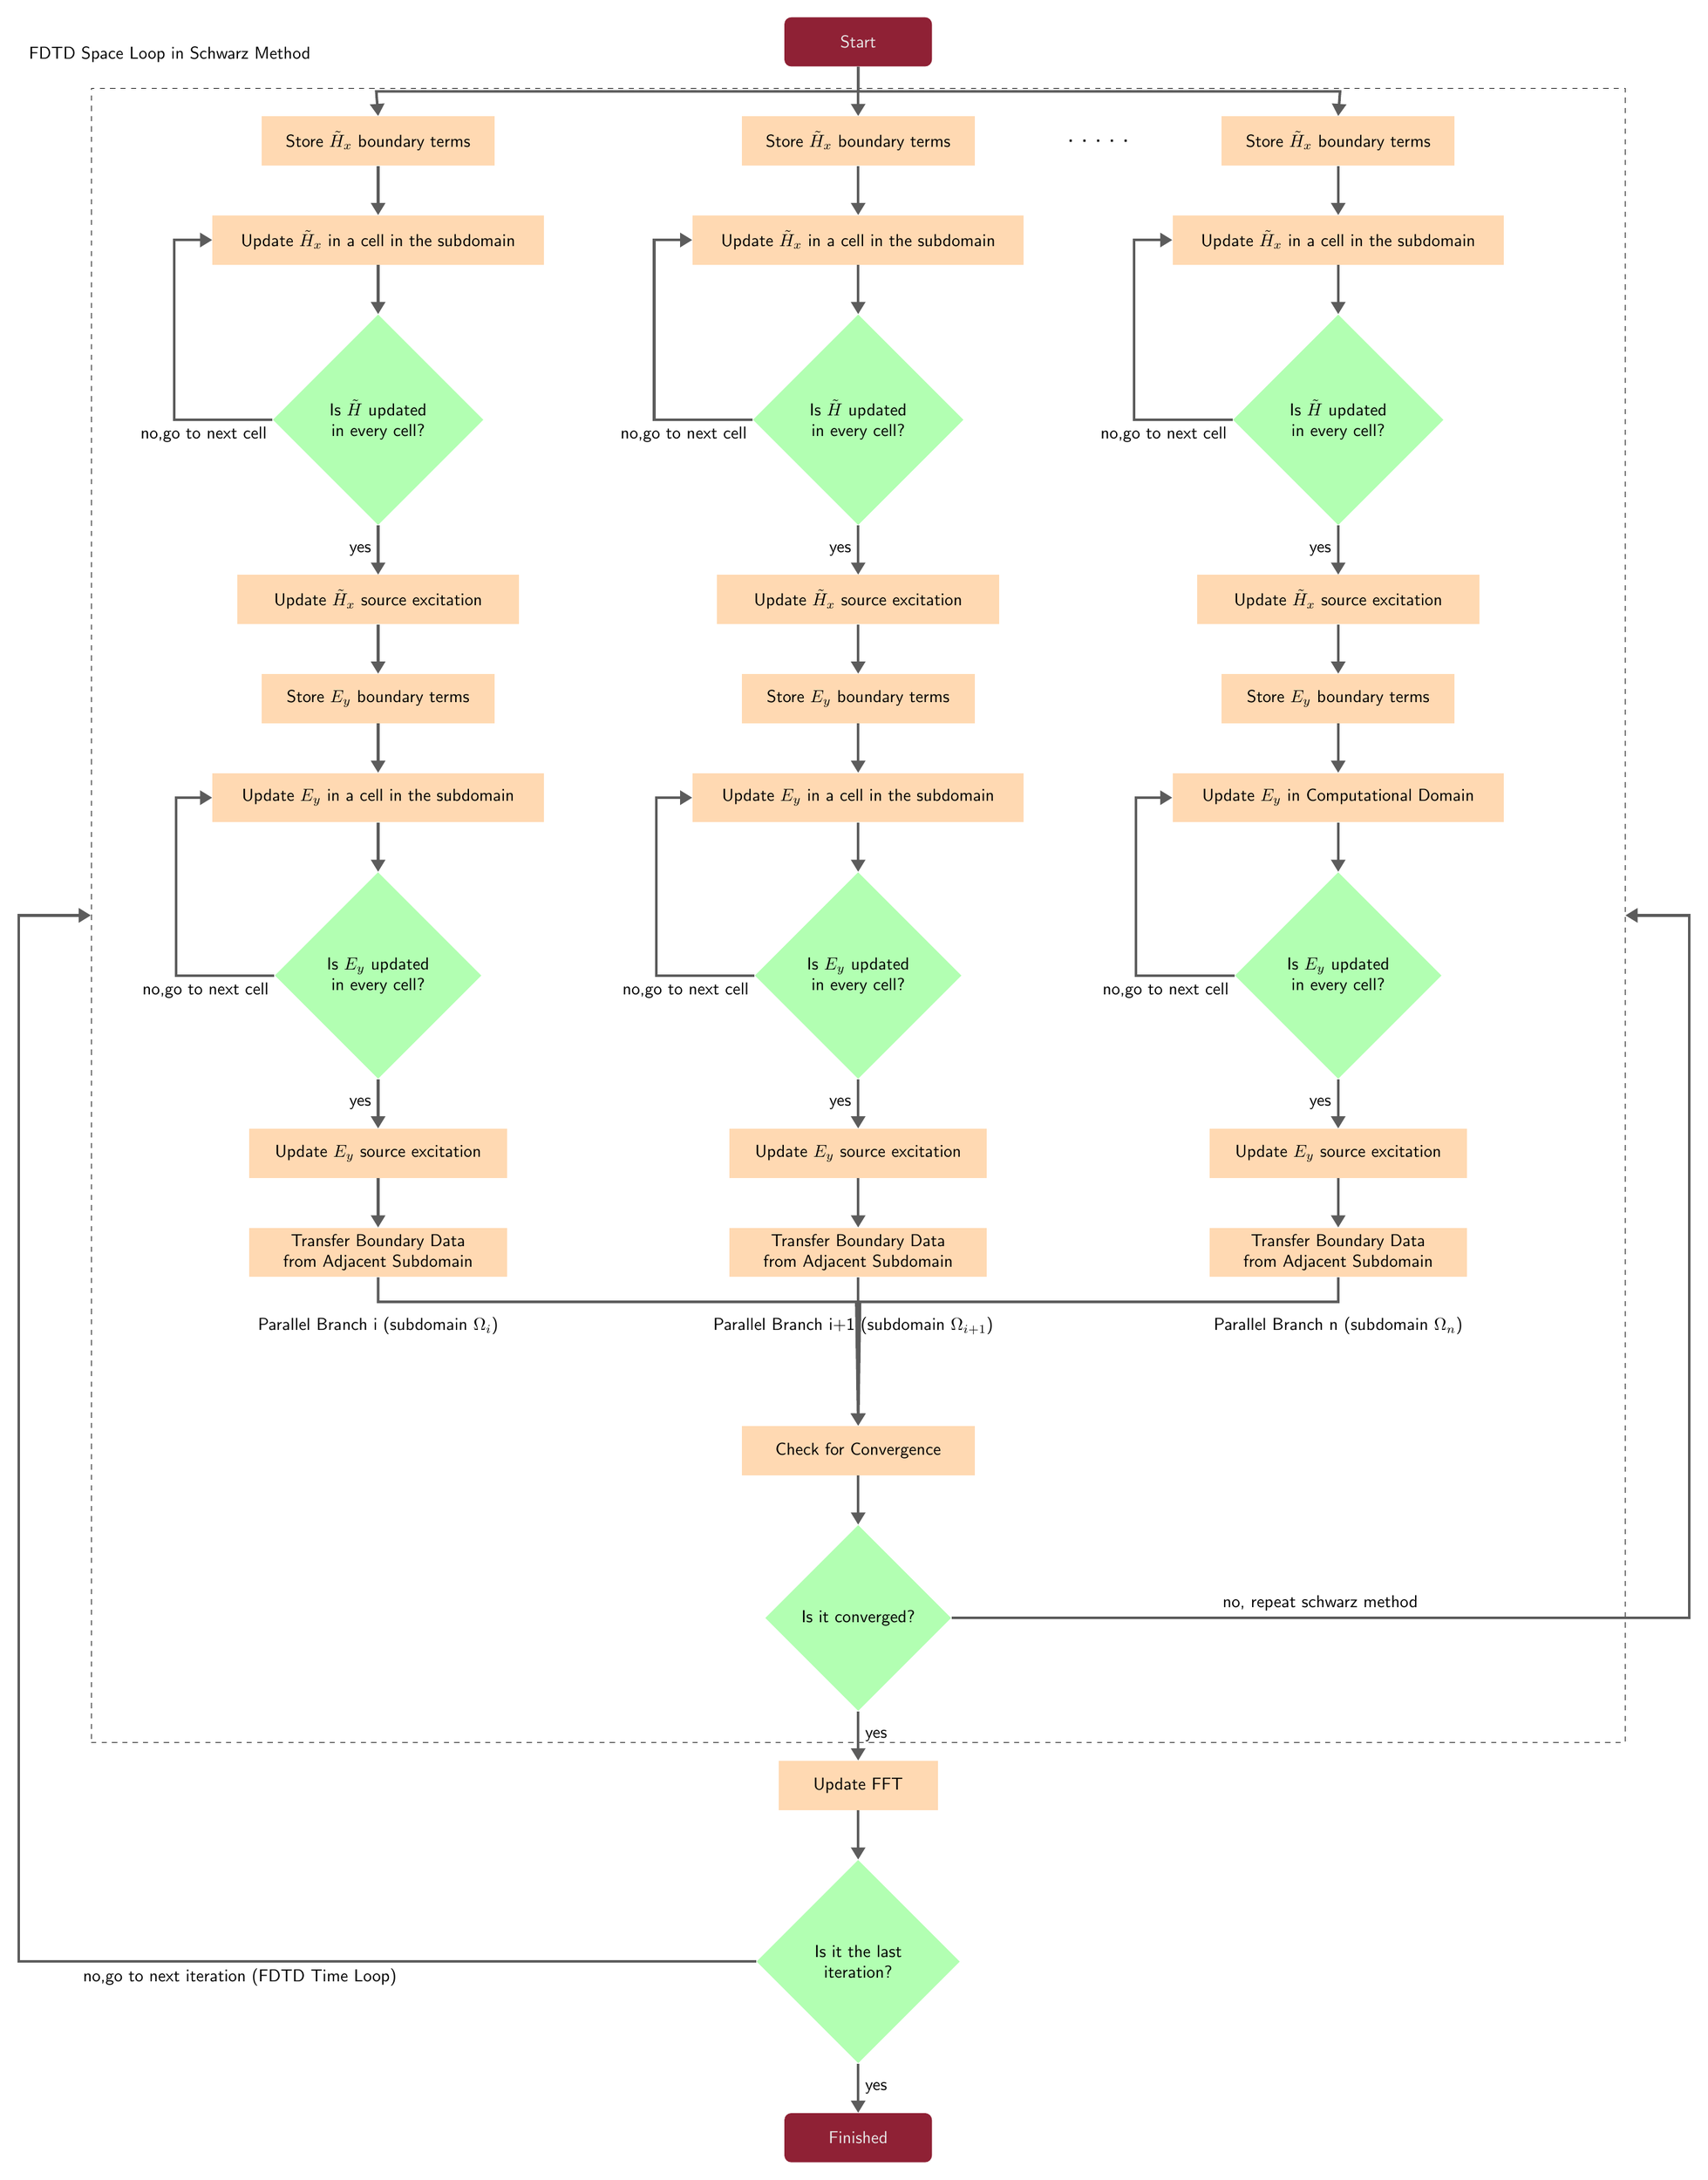
\begin{tikzpicture}


	\centering
	\sffamily

	%Creating the elements in the Schwarz Alternating Method
	%Center Column
	\node (start) [startstop] {Start};
	%\node (solve_pde_C) [process, below= of start_algo] {Solve PDE on subdomain 2};
	\node (store_Hboundary_terms_C) [process,text width=4.5cm, below=of start] {Store $\tilde{H}_x$ boundary terms};
	\node (update_H_C) [process,text width=6.5cm, below= of store_Hboundary_terms_C] {Update $\tilde{H}_x$ in a cell in the subdomain};
	\node (is_H_finished_C) [decision, below= of update_H_C] {Is $\tilde{H}$ updated in every cell?};
	\node (update_source_H_C) [process,text width=5.5cm, below= of is_H_finished_C] {Update $\tilde{H}_x$ source excitation};
	\node (store_Eboundary_terms_C) [process,text width=4.5cm, below=of update_source_H_C] {Store $E_y$ boundary terms};
	\node (update_E_C) [process,text width=6.5cm, below= of store_Eboundary_terms_C] {Update $E_y$ in a cell in the subdomain};
	\node (is_E_finished_C) [decision, below= of update_E_C] {Is $E_y$ updated in every cell?};
	\node (update_source_E_C) [process,text width=5cm, below= of is_E_finished_C] {Update $E_y$ source excitation};
	%\node (solve_ext_BC_C) [process, below= of update_source_E_C] {Set Ext. Boundary Conditions of Subdomain};
	
	\node (transfer_data_C) [process,text width=5cm,below = of update_source_E_C] {Transfer Boundary Data from Adjacent Subdomain};
%	\node (filler_3) [filler, below= of transfer_data_C] {  };
	%Filler Column
	\node (filler_2) [filler, left= of store_Hboundary_terms_C] {  };
	
	%Left Column
	%\node (solve_pde_L) [process, left= of solve_pde_C] {Solve PDE on subdomain 1};
	\node (store_Hboundary_terms_L) [process,text width=4.5cm, left = of filler_2] {Store $\tilde{H}_x$ boundary terms};
	\node (update_H_L) [process,text width=6.5cm, below= of store_Hboundary_terms_L] {Update $\tilde{H}_x$ in a cell in the subdomain};
	\node (is_H_finished_L) [decision, below= of update_H_L] {Is $\tilde{H}$ updated in every cell?};
	\node (update_source_H_L) [process,text width=5.5cm, below= of is_H_finished_L] {Update $\tilde{H}_x$ source excitation};
	
	\node (store_Eboundary_terms_L) [process,text width=4.5cm, below=of update_source_H_L] {Store $E_y$ boundary terms};
	\node (update_E_L) [process,text width=6.5cm, below= of store_Eboundary_terms_L] {Update $E_y$ in  a  cell in the subdomain};
	\node (is_E_finished_L) [decision, below= of update_E_L] {Is $E_y$ updated in every cell?};
	\node (update_source_E_L) [process, text width=5cm,below= of is_E_finished_L] {Update $E_y$ source excitation};
	%\node (solve_ext_BC_L) [process, below= of update_source_E_L] {Set Ext. Boundary Conditions of Subdomain};
	\node (transfer_data_L) [process,text width=5cm, below = of update_source_E_L] {Transfer Boundary Data from Adjacent Subdomain};
	
	%Filler Column
	\node (filler_1) [filler, right= of store_Hboundary_terms_C] {\textbf{. . . . .}};

		
	
	%Column 4
	%\node (solve_pde_R) [process, right= of filler_1] {Solve PDE on subdomain N};
	\node (store_Hboundary_terms_R) [process,text width=4.5cm, right = of filler_1] {Store $\tilde{H}_x$ boundary terms};
	\node (update_H_R) [process,text width=6.5cm, below= of store_Hboundary_terms_R] {Update $\tilde{H}_x$ in  a cell  in the subdomain};
	\node (is_H_finished_R) [decision, below= of update_H_R] {Is $\tilde{H}$ updated in every cell?};
	\node (update_source_H_R) [process,text width=5.5cm, below= of is_H_finished_R] {Update $\tilde{H}_x$ source excitation};
	\node (store_Eboundary_terms_R) [process,text width=4.5cm, below=of update_source_H_R] {Store $E_y$ boundary terms};
	\node (update_E_R) [process,text width=6.5cm, below= of store_Eboundary_terms_R] {Update $E_y$ in Computational Domain};
	\node (is_E_finished_R) [decision, below= of update_E_R] {Is $E_y$ updated in every cell?};
	\node (update_source_E_R) [process,text width=5cm, below= of is_E_finished_R] {Update $E_y$ source excitation};
	%\node (solve_ext_BC_R) [process, below= of update_source_E_R] {Set Ext. Boundary Conditions of Subdomain};
	\node (transfer_data_R) [process, text width=5cm,below = of update_source_E_R] {Transfer Boundary Data from Adjacent Subdomain};
	%Filler Column
	\node (filler_3) [filler, below= of transfer_data_C] { };
	\node (check_conv) [process, text width=4.5cm,below= of filler_3] {Check for Convergence};
	\node (domain_conv) [decision,below=of check_conv] {Is it converged?};
	\node (update_FFT) [process, below = of domain_conv] {Update FFT};
	\node (last_iter) [decision, below = of update_FFT] {Is it the last iteration?};
    \node (finished) [startstop, below= of last_iter] {Finished};
    
    \node[fit={ (update_source_H_R) 
                (store_Hboundary_terms_R) 
                (update_H_R) 
                (store_Eboundary_terms_R)
                (update_E_R)
                (update_source_E_R)
                %(solve_ext_BC_R)
                (transfer_data_R)
                (store_Hboundary_terms_C) 
                (update_H_C) 
                (update_source_H_C)
                (store_Eboundary_terms_C)
                (update_E_C)
                (update_source_E_C)
                %(solve_ext_BC_C)
                (transfer_data_C)
                (store_Hboundary_terms_L)
                (update_H_L)
                (update_source_H_L)
                (store_Eboundary_terms_L)
                (update_E_L)
                (update_source_E_L)
                %(solve_ext_BC_L)
                (transfer_data_L)
                (check_conv)
                (domain_conv)
                (filler_1)}, dashed, draw,fit margins={left=35pt,right=35pt,bottom=9pt,top=8pt}] (fdtd_space_schwarz){};
    \node  (fdtd_space_schwarz_title) at ([shift={(-14,17.5)}]fdtd_space_schwarz) {FDTD Space Loop in Schwarz Method};
    
    \node  (subdomain_L) at ([shift={(0,-1.5)}]transfer_data_L) {Parallel Branch i (subdomain $\Omega _i$)};
    \node  (subdomain_C) at ([shift={(-.1,-1.5)}]transfer_data_C) {Parallel Branch i+1 (subdomain $\Omega _{i+1}$)};
    \node  (subdomain_R) at ([shift={(0,-1.5)}]transfer_data_R) {Parallel Branch n (subdomain $\Omega _{n}$)};
	%Draw the arrows for the flowchart
	%Draw multi-headed arrow
	\draw [arrow_cap] (start.south) -- (store_Hboundary_terms_C.north);
	\draw [arrow_cap] (start.south) |- ++(-9.8,-.5) -- (store_Hboundary_terms_L.north);
	\draw [arrow_cap] (start.south) |- ++(9.8,-.5) -- (store_Hboundary_terms_R.north);
	
	%Draw arrows in column 1
	\draw [arrow_cap] (store_Hboundary_terms_L) -- (update_H_L);
	\draw [arrow_cap] (update_H_L) -- (is_H_finished_L);
	\draw [arrow_cap] (is_H_finished_L) -- node[anchor=east]{yes} (update_source_H_L);
	\draw [arrow_cap] (is_H_finished_L.west) |-  node[anchor=north,pos=.85]{no,go to next cell} ++(-2,0) |-  (update_H_L.west);
	\draw [arrow_cap] (update_source_H_L) -- (store_Eboundary_terms_L);
	\draw [arrow_cap] (store_Eboundary_terms_L) -- (update_E_L);
	\draw [arrow_cap] (update_E_L) -- (is_E_finished_L);
	\draw [arrow_cap] (is_E_finished_L) -- node[anchor=east]{yes} (update_source_E_L);
	\draw [arrow_cap] (is_E_finished_L.west) |-  node[anchor=north,pos=.85]{no,go to next cell} ++(-2,0) |-  (update_E_L.west);
	\draw [arrow_cap] (update_source_E_L) -- (transfer_data_L);
	
	%Draw arrows in column 2
	\draw [arrow_cap] (store_Hboundary_terms_C) -- (update_H_C);
	\draw [arrow_cap] (update_H_C) -- (is_H_finished_C);
	\draw [arrow_cap] (is_H_finished_C) -- node[anchor=east]{yes} (update_source_H_C);
	\draw [arrow_cap] (is_H_finished_C.west) |-  node[anchor=north,pos=.85]{no,go to next cell} ++(-2,0) |-  (update_H_C.west);
	\draw [arrow_cap] (update_source_H_C) -- (store_Eboundary_terms_C);
	\draw [arrow_cap] (store_Eboundary_terms_C) -- (update_E_C);
	\draw [arrow_cap] (update_E_C) -- (is_E_finished_C);
	\draw [arrow_cap] (is_E_finished_C) -- node[anchor=east]{yes} (update_source_E_C);
	\draw [arrow_cap] (is_E_finished_C.west) |-  node[anchor=north,pos=.85]{no,go to next cell} ++(-2,0) |-  (update_E_C.west);
	\draw [arrow_cap] (update_source_E_C) -- (transfer_data_C);
	
	
	%Draw arrows in column 4
	\draw [arrow_cap] (store_Hboundary_terms_R) -- (update_H_R);
	\draw [arrow_cap] (update_H_R) -- (is_H_finished_R);
	\draw [arrow_cap] (is_H_finished_R) -- node[anchor=east]{yes} (update_source_H_R);
	\draw [arrow_cap] (is_H_finished_R.west) |-  node[anchor=north,pos=.85]{no,go to next cell} ++(-2,0) |-  (update_H_R.west);
	\draw [arrow_cap] (update_source_H_R) -- (store_Eboundary_terms_R);
	\draw [arrow_cap] (store_Eboundary_terms_R) -- (update_E_R);
	\draw [arrow_cap] (update_E_R) -- (is_E_finished_R);
	\draw [arrow_cap] (is_E_finished_R) -- node[anchor=east]{yes} (update_source_E_R);
	\draw [arrow_cap] (is_E_finished_R.west) |-  node[anchor=north,pos=.85]{no,go to next cell} ++(-2,0) |-  (update_E_R.west);
	\draw [arrow_cap] (update_source_E_R) -- (transfer_data_R);
	
	
	
	%Draw from parallel to serial
	
	\draw [arrow_cap] (transfer_data_C.south) -- (check_conv.north);
	\draw [arrow_cap] (transfer_data_L.south) |- ++(9.8,-.5) -- (check_conv.north);
    \draw [arrow_cap] (transfer_data_R.south) |- ++(-9.8,-.5) -- (check_conv.north);
    \draw [arrow_cap] (check_conv.south) -- (domain_conv.north);
    
    \draw [arrow_cap] (domain_conv) -- node[anchor=west] {yes} (update_FFT);
    \draw [arrow_cap] (update_FFT) -- (last_iter);
    \draw [arrow_cap] (last_iter) -- node[anchor=west]{yes}(finished);
    \draw [arrow_cap] (domain_conv.east) |- node[anchor=south,pos=.75]{no, repeat schwarz method}  ++(15,0) |-  (fdtd_space_schwarz.east);
    \draw [arrow_cap] (last_iter.west) |- node[anchor=north,pos=.85]{no,go to next iteration (FDTD Time Loop)} ++(-15,0) |- (fdtd_space_schwarz.west);
    
    \end{tikzpicture}
    }
    \caption{FDTD-Schwarz Algorithm Flowchart}
    \label{fig:fdtd_schwarz_flowchart}
\end{figure} 

The combined algorithm has three major processes,
\begin{enumerate}
    \item FDTD time loop
    \item Schwarz Algorithm
    \item FDTD space loop
\end{enumerate}

To start, after the pre-processing is done, the algorithm will enter the FDTD Time Loop which involves these steps:
\begin{enumerate}
    \item Schwarz Algorithm
    \item Updating the Fourier Transform and checking the stop condition
\end{enumerate}

Similar to what was done in the FDTD algorithm, the FDTD time loop is the outer loop of the algorithm that iterates through time which means that after every iteration, there will be a 'snapshot' of the current field values in the current time step. Since the Schwarz Algorithm is integrated, it will be done for every iteration to make sure that each 'snapshot' in every time step converges. After the Schwarz algorithm is done in this iteration, the Fourier transform is updated for the reflectance and transmittance coefficients. Fourier transform is outside of the Schwarz algorithm to prevent wasteful computation since after every Schwarz Algorithm run, the solution is converges unlike if after every iteration inside the Schwarz the Fourier transform is included, there will be unnecessary computations since the Fourier Transform of the fields will be wasted if the subdomains do not converges. The stop condition is similar to the stop condition of the FDTD algorithm where the algorithm will stop and proceed to post-processing if the current time step is equal to the last time step specified in the pre-processing stage. 

The Schwarz Algorithm and FDTD Space Loop are integrated with each other such that the first step in the Schwarz loop in subsection \ref{subsec:schwarz} where the PDEs in the subdomains are solved is the FDTD Space Loop. In simpler terms, the first half of Schwarz loop where the operation can be done asynchronous with respect to each subdomain is the FDTD Space Loop because it will solve for the PDEs (FDTD update equations) and solve the external boundary conditions of each subdomain. 

The steps in Schwarz Algorithm (in the FDTD-Schwarz Algorithm):
\begin{enumerate}
    \item FDTD space loop
    \item Transfer the data from the adjacent subdomain/s to the inner boundary of the subdomain
    \item Check for convergence of each subdomain
\end{enumerate}

The second half of the algorithm will still be done synchronously with respect to each subdomain because it needs the updated values in each subdomain for the internal boundaries of the subdomains. After the transfer of data, the convergence will be validated using the error equation and the condition in equation \ref{eq:converge_cond} similar to the process in Schwarz Algorithm. At the end of Schwarz-FDTD Space Loop, if the solution converges, the algorithm will proceed to step 2 of FDTD Time Loop, otherwise the algorithm will start step 1 of Schwarz-FDTD Space Loop and run the FDTD Space Loop again.

The project will implement this combined algorithm because this algorithm provides FDTD to validate the results of its parallel configuration. The convergence of the solution in each iteration will be important because the results of each subdomain might not be correct if the convergence is not validated in every time step.


\subsection{Simulation Models} \label{meth:simmodels}

The simulation models that will be used in the project will be discussed here. These models are \textbf{plane wave propagation in different media} and \textbf{bragg grating}.\\


\noindent
\textbf{Plane wave propagation in various media}
\\


\begin{figure}[H]
     \centering
     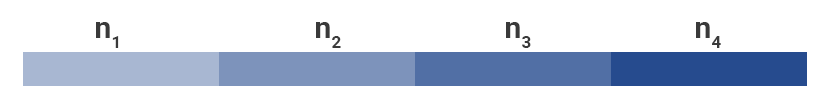
\includegraphics[width=\textwidth]{images/different_medias.png}
     \caption{Different materials with increasing refractive indices from left to right}
     \label{fig:1st_model}
 \end{figure}

Plane wave propagation is one of the simplest EM simulation that can be done in FDTD. As shown on Figure \ref{fig:1st_model}, the different materials are stacked side to side such that their refractive index is increasing from left to right.\\

 \noindent
 \textbf{Bragg Grating}

 \begin{figure}[H]
     \centering
     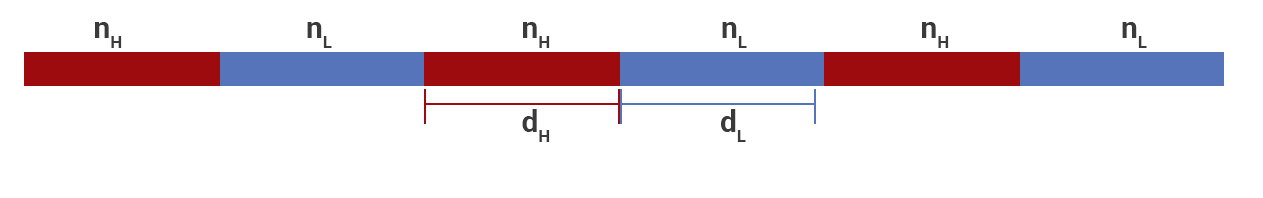
\includegraphics[width=\textwidth]{images/bragg_gratings.png}
     \caption{Bragg grating in 1D}
     \label{fig:2nd_model}
 \end{figure}

 This type of grating uses an alternating configuration of different materials with high and low refractive index \cite{Rumpf092014} as shown in Figure \ref{fig:2nd_model}. This type of grating is primarily used in preventing certain wavelengths of electromagnetic waves from passing through the grating \cite{Allil2017}. This model is selected as one of the simulation models that will be used in the project since this can be done on 1D assuming that the other directions (y and z axis) have similar refractive index.

\begin{align}
    &d_H\,=\,\frac{\lambda}{4n_H}\label{eq:dH}\\
    &d_L\,=\,\frac{\lambda}{4n_L}
    \label{eq:dL}
\end{align}

The design of a Bragg grating model can be done by adjusting thickness of each material based on \ref{eq:dH} and \ref{eq:dL} since the wavelength $ \lambda $ is proportional to the thickness of the two materials ($d_H,d_L$). This means that the higher the target frequency to reflect, thinner thickness for each material in the grating is needed.


\subsection{Machine Configuration}

The hardware specifications of the machine that will be used in this project are not yet determined due to different constraints but the minimum general specifications are determined and shown on the table below:

\begin{table}[H]
\caption{Machine Configuration  \label{tab:software_specs}}

\centering{}%
\begin{tabular}{|c|c|}
\hline 
\textbf{Specification} & \textbf{Value} \tabularnewline
\hline 
\hline 
 Operating System &  Linux (Ubuntu) \tabularnewline
\hline 
 CPU & Multi-core processor \tabularnewline
\hline 
 Programming Language/s & C++ and Python 3 \tabularnewline
\hline 
\end{tabular}
\end{table}

The operating system chosen was Linux (specifically Ubuntu) because of convenience but it is expected that the code base will be compatible with any Linux distributions as long as the dependencies are properly installed. The CPU of the machine must be a multi-core processor since the project can take advantage of the number of cores in increasing the amount of subdomain in each simulation. The programming languages used will be C++ and Python in combination with each other since C++ is generally faster in computing then Python \cite{Tamimi2020} while Python's modules in data visualization is easier to use than C++'s libraries.

\section{Implementation}

In this part, the specific details of the algorithm as well as simulation parameters will be discussed in detail as well as the system's input/output handling for ease of use. The main algorithm process will not be discussed here because it is already discussed in section \ref{sec:design}.

\subsection{Pre-Processing}

In the pre-processing stage, the initialization of the simulation parameters as well as the input handling of the system occurs. There are two main parts in the pre-processing: 
\begin{enumerate}
    \item Input handling; and
    \item Initialization of simulation parameters and computational domain.
\end{enumerate}

\subsubsection{Input Handling}

In this part, the details about the input files and formats will be discussed. The file type of the input file is a \textbf{.csv file}. This file type was chosen because it can be easily read by the system through built-in libraries for simpler parsing. The input name of the file must be in this format ``\textbf{sim\_model.csv}"The format of the csv file will be as shown below:

\begin{table}[H]
\caption{Format of Input File \label{tab:input_file}}

\centering{}%
\begin{tabular}{|c|c|c|c|}
\hline 
\textbf{Column 1} & \textbf{Column 2} & \textbf{Column 3} & \textbf{Column 4} \tabularnewline
\hline 
\hline 
$d_{1}$ & $\mu _{1}$ & $\epsilon _{1}$ & $f_{MAX}$ \tabularnewline
$d_{2}$ & $\mu _{2}$ & $\epsilon _{2}$ & source \tabularnewline
$d_{3}$ & $\mu _{3}$ & $\epsilon _{3}$ & $n_{model}$ \tabularnewline
$d_{4}$ & $\mu _{4}$ & $\epsilon _{4}$ & $t_{sim}$ \tabularnewline
. & . & . & \tabularnewline
. & . & . & \tabularnewline
. & . & . & \tabularnewline
$d_{n}$ & $\mu _{n}$ & $\epsilon _{n}$ &  \tabularnewline

\hline 
\end{tabular}
\end{table}

So, in this format, columns 1 to 3 describe the model's layer where each row corresponds to a model's thickness in meters ($d$), magnetic permeability ($\mu$), electric permittivity ($\epsilon$), and n specifies how many layers in the simulation model. Column 4 describes the source excitation that will be used in the simulation where $f_{MAX}$ is the maximum frequency that will be included in the source while source type specifies whether the source is a gaussian source (integer 0) or sinusoidal source (integer 1) as well as the total number of layers (n) of the model and $t_{sim}$ specifies how long the simulation time (in seconds). The input file does not indicate how many cells will have in each layer because the cell size $\Delta z$ is computed at every simulation so it is better to specify the physical distance of the layers in the simulation model.

\subsubsection{Initialization of simulation parameters}

The simulation parameters that are not needed to be computed at every iteration are done here to save computation time. The list of simulation parameters initialize are shown below:

\begin{table}[H]
\caption{Initialized Simulation Parameters \label{tab:init_param}}

\centering{}%
\begin{tabular}{|c|c|}
\hline 
\textbf{Parameter} &\tabularnewline
\hline 
\hline 
$c_0$ & 299792458.0 \tabularnewline
\hline 
$\epsilon_0$ & 8.8541878128e-12 \tabularnewline
\hline 
$\mu _0$ & 1.25663706212e-06 \tabularnewline
\hline 
Boundary terms  & Array of size (1,2) \tabularnewline
\hline 
$\Delta z$ & 0 \tabularnewline
\hline 
$\Delta t$ & 0 \tabularnewline
\hline 
Source & Vector \tabularnewline
\hline 
Update Coefficients (for E and $\tilde{H}$) & Vector \tabularnewline
\hline 
\end{tabular}
\end{table}

So, the initialization of these parameters are done before the simulation proper to lessen computation time per iteration since they are only needed to be initialized once. The following subsections discuss how the cell size and time step and update coefficients are computed while the computation for the source excitation will be discussed in the next section.

\subsubsection{Setup of Computational Domain}\label{subsec:setup_comp_domain}

The computational domain is the space where the electric and magnetic fields are computed in the FDTD algorithm as well as where the simulation model is located. To set up the computational domain, there are several considerations that need to be taken into account to ensure the convergence of the simulation as well as to prevent numerical dispersion as discussed in \cite{Rumpf082014}.\\

\noindent \textbf{Grid Dispersion}

In computing for a good grid resolution for the computational domain, two factors are usually considered: (1) Minimum Wavelength and (2) Minimum Dimension \cite{Rumpf082014}. This is related to the concept of grid dispersion that can cause numerical instability in FDTD. This project will only deal with uniform grid resolution (meaning constant delta z) so that the computations will be simplified in 1 dimension context. 


\begin{align}
    \lambda _{min}\,=\,\frac{c_0}{f_{max}n_{max}}
    \label{eq:min_wavelen}
\end{align}

The minimum wavelength is usually considered when computing the grid resolution to prevent numerical dispersion. The computation of the minimum wavelength for the grid size is done because the smallest wavelength in the FDTD simulation must be sampled properly to satisfy Nyquist sampling theorem \cite{Elsherbeni2015}. The minimum wavelength is computed using equation \ref{eq:min_wavelen} that considers the max frequency needed in the simulation $f_{MAX}$ and the largest refractive index in the computational domain $n_{MAX}$. 


\begin{align}
    \Delta z_{\lambda}\,\approx \, \frac{\lambda _{min}}{N_{\lambda}},\,\,\,N_{\lambda}\,\geq\,10
    \label{eq:dz_for_wavelen}
\end{align}

The rule of thumb in computing the grid resolution when considering the minimum wavelength is that the number of cells ($N_{\lambda}$) that resolve the minimum wavelength must at least be 10 cells. This can be increased depending on the type of material in the computational domain. For example, the recommended number of cells $N_{\lambda}$ for low contrast dielectrics are 10 - 20, 20 - 30 for high contrast dielectrics, 40 - 60 for metallic materials, and 100 - 200 for plasmonic devices. In this project, the focus will be on dielectrics so the number of cells will be at a maximum of 40 cells to ensure that the refractive index of most dielectrics are considered.\\



\noindent
\textbf{Device Dimension}

This part considers the simulation model used in the computational domain. The consideration with regards to the device dimensions are that the minimum dimensions in the simulation model must be resolved in the grid resolution. The minimum dimension $d_{min}$ of the simulation model is the smallest feature of the model and in the context of the project, since the scope is only on one dimension (z dimension), this means that the minimum thickness of a layer should be considered \cite{Rumpf062014}.

\begin{align}
    \Delta z_{d}\,\approx \, \frac{d_{min}}{N_{d}},\,\,\,N_{d}\,\geq \,1
    \label{eq:dz_for_device}
\end{align}

The grid resolution due to the minimum dimension in the model is shown in \ref{eq:dz_for_device}. As shown, the minimum dimension of the model is considered by setting the number of cells that represent the minimum dimension to at least 1 cell. However, it is recommended to set it at $N_d$ = 4 so that the features of the model are properly represented \cite{Rumpf062014}. 


\begin{align}
    \Delta z \, =\, min[\Delta z_{\lambda},\Delta z_{d}]
\end{align}

The final grid resolution can be computed by selecting the minimum grid resolution between the grid resolution due to minimum wavelength and the grid resolution due to minimum model dimension. This cell size or grid resolution will be used in the FDTD simulation.

There is another consideration in grid resolution, the critical dimension of the model, which is the actual dimension (total dimension) of the simulation model. This consideration will not be considered in this project because of the project's scope in 1D and the models used fit in the Yee cells without any problem. This consideration is important when creating a higher dimension FDTD simulation because the cells might not have homogenous material if the critical dimension is not considered. This consideration makes sure that the model in the computational domain fits each cell properly such that the border of the model is also the border of a Yee cell.\\


\noindent
\textbf{Courant-Friedrichs-Lewy Stability Criterion (CFL Condition)}

In an FDTD simulation, the change in electric and magnetic fields in a cell is only felt by the adjacent cells in each iteration, this results in the propagation of the fields to be 1 cell per 2 time step because of the staggered scheme of the electric and magnetic fields in the computational domain. This is also related to the fact that the speed of EM waves are different in different media and the maximum speed an EM wave can propagate is its speed in vacuum $c_0$. This is described by the \textit{Courant Stability Criterion}:


\begin{align}
   &\Delta t_{3D}\,<\,\frac{n_{min}}{c_0 \sqrt{\frac{1}{(\Delta x)^2}\,+\,\frac{1}{(\Delta y)^2}\,+\,\frac{1}{(\Delta z)^2}}}\\
   &\Delta t_{1D}\,<\,\frac{n_{min}\Delta z}{2c_0} \label{eq:delta_t}
\end{align}

The basic description of CFL condition (as shown on equation \ref{eq:delta_t}) for FDTD is that the time step is restricted by the speed by which the EM wave is propagating in the highest speed (lowest refractive index) and the size of each cell in the FDTD grid \cite{Elsherbeni2015} and \cite{Inan2011}. The constant coefficient 0.5 is added in the CFL condition as a safety margin to make sure that the simulation will be stable \cite{Rumpf062014}. If the CFL is not satisfied, the FDTD simulation will be unstable as time passes because as explained previously, in FDTD an EM wave cannot physically travel in more than one cell in two time steps \cite{Houle2019}. The CFL condition prevents instability in FDTD simulation by restricting the size of the time step based on the inherent instability of FDTD if the EM waves travel in more than one cell size.\\

\noindent
\textbf{Layout of Computational Domain}\\

\noindent
\textit{Serial Configuration}\\

After resolving the grid resolution and time resolution of the computational domain, the whole computational domain can be created. Following \cite{Rumpf072014}, when creating the computational domain, adding spacers (cells that have a refractive index of air/vacuum) can be used so that there is a space between the boundary of the computational domain and the simulation model. This will help in the visualization of the reflected fields and transmitted fields after it hits the simulation model or passes through it. 

\begin{figure}[H]
    \centering
    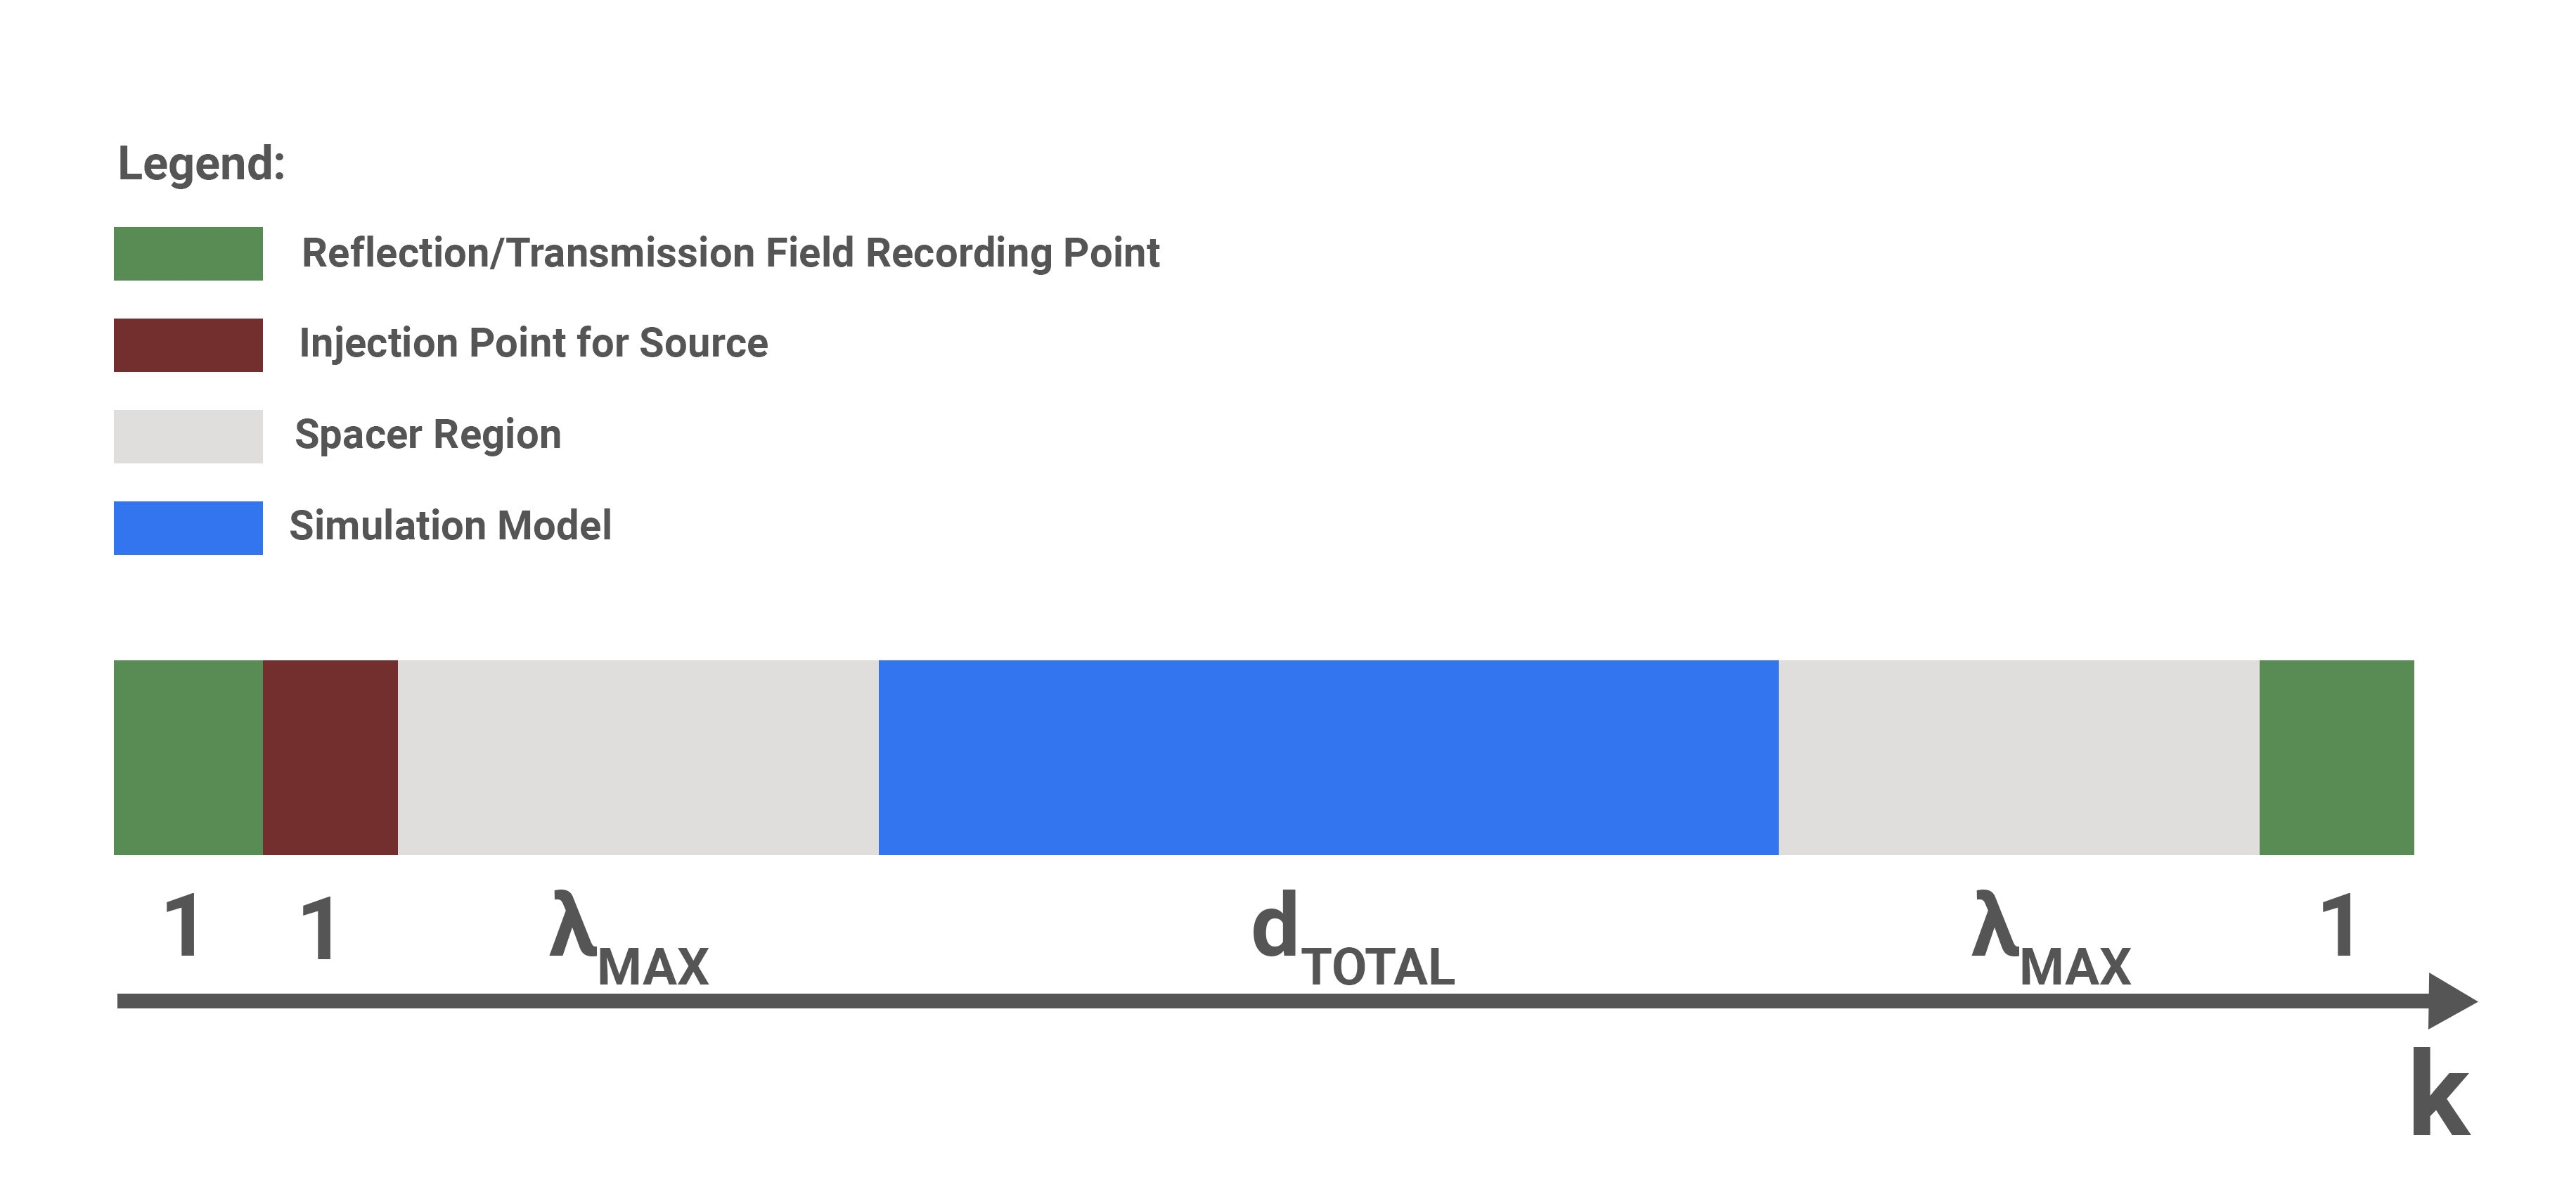
\includegraphics[width=\textwidth]{images/layout_computational_domain.png}
    \caption{Layout of Computational Domain for 1D FDTD}
    \label{fig:layout_comp_domain}
\end{figure}

As shown in Figure \ref{fig:layout_comp_domain}, The first and last cells are the reflection and the transmission recording point of the simulation (this will be further explained in the next subsection on why it works). The simulation model is in the center of the computational domain and the spacer regions, which at least have a minimum size of $\lambda_{MAX}$ is on either side of the simulation model. The point of injection for the source is located at the left side of the computational domain, near the reflection recording point. The selected sizes are also shown on the figure above as shown where the recording point and the injection point of the source in the simulation is only 1 cell, while the spacer region is at least the size of the largest wavelength in the source while the size of the simulation model $d_{TOTAL}$ is dependent on the input file. 

Another function of the spacer region in the computational domain is to make the number of cells in the computational domain divisible to 2 so that the partitioning of the computational domain in the parallel configuration is easy and less prone to more complexities such that the subdomains have equal lengths.\\


\noindent
\textit{Parallel Configuration}

The process of creating and layout of the computational domain in the parallel configuration is the same as the serial configuration. An additional process is added after the layout of the computational domain is created. This process is the \textit{partitioning of the computational domain into subdomains}. The number of subdomains will correspond to how many processes will be run in parallel in the FDTD simulation. The selected formula for getting the number of subdomains is shown below:

\begin{align}
    No. of subdomain\,=\, 2^{x}, \,\,\, x \,\in\, [1,5] \label{eq:no_subd}
\end{align}

This equation (\ref{eq:no_subd}) such that x is the order of simulations that will be done in this project (i.e. x = 1 is the first simulation run for parallel configuration where the number of subdomains will be 2). This ensures that the number of subdomains will always be even and the computational domain can be divided equally (every subdomain has equal length) so complexities on the length of subdomain that is not an integer value is prevented. 

After the cell size and time step are computed, the update coefficients (see equation \ref{eq:update_coeffE} and \ref{eq:update_coeffH}) can be calculated since they are dependent on these parameters. These will be a vector that have different values depending on what the refractive index is on each cell. These will be used in the update equations (equations \ref{eq:updateE} and  \ref{eq:updateH}) in order for the FDTD to take into account the material properties that the EM wave is propagating into while the time step and cell size is still considered.

\subsection{Simulation Proper}

This subsection will discuss the specific configurations of the two main methods used in this project. First, the FDTD Method's assumptions, boundary conditions, and source excitations are discussed. Second, the Schwarz Alternating Method's assumptions, initial guess, boundary conditions, and the convergence of the computational domain.

\subsubsection{FDTD Algorithm}

In subsection \ref{subsec:fdtd_method} the algorithm is discussed in the context of a one dimensional computational domain. The boundary conditions and source excitations that will be used in this project is discussed. %However, the assumptions that are considered in this method are still not discussed. This subsection discusses the assumption in the FDTD algorithm. These are:

%\begin{enumerate}
%    \item The materials in the computational domain are linear, homogeneous, isotropic, and lossless.
%    \item Any change in x or y direction (derivatives) are 0. This implies that the computations in the computational domain are restricted in 1 dimension (z-direction).
%    \item There are no electromagnetic sources inside the computational domain. This implies that the sources that will be used in this project are plane waves where the sources of these waves are far away from the computational domain.

%\end{enumerate}

%These three assumptions are used in the FDTD algorithm to simplify the calculations, and also the code base. \\
\noindent
\textbf{Boundary Conditions}

As explained in subsection \ref{subsec:fdtd_method}, there is a boundary in the computational domain because the simulation cannot extend the space infinitely so the computational domain is a closed space. However, to make the simulation behave similar to reality, the boundaries must act like the plane waves will not reflect in the boundaries and pass through them, making the computational domain like an open space. There are simpler boundary conditions (Dirichlet Boundary Conditions) that act like a barrier that reflects any EM wave that will not be discussed here but it will be shown in Chapter \ref{cha:Prelims}.\\


\noindent
\textit{Perfectly Absorbing Boundary Condition (PABC)}

PABC is a boundary condition used in FDTD as discussed by \cite{Rumpf062014} and \cite{Houle2019}, that takes advantage of how the EM fields move in the Yee grid. The problem of FDTD update equations is that they are dependent on the adjacent cells. At the left side boundary of the computational domain (k = 0), the electric field update equation (equation \ref{eq:updateE}) shows that it requires magnetic field values outside the computational domain (k = -1) . Similarly, at the right side boundary of the computational domain ($k=N_z$), the magnetic field update equation ( equation \ref{eq:updateH}) shows that it requires electric field values outside the computational domain ($k = N_z +1$)\cite{Rumpf062014}.

As discussed in subsection \ref{subsec:setup_comp_domain}, the EM waves cannot travel more than one cell per two time step \cite{Houle2019} in FDTD so since the movement of the electric and magnetic fields are known, predicting the fields at the boundary by saving the value at the boundary in previous timesteps can make the fields propagate outside the computational domain. This is done in the FDTD algorithm (see figure \ref{fig:fdtd_flowchart}) by saving the boundary terms in each iteration \cite{Rumpf062014}. The update equations for the PABC boundary condition used  are shown below:


\begin{align}
    &z_{low}\,=\,[0,0],\,\,\,z_{low}[0]\,=\,z_{low}[1],\,\,\,z_{low}[1]\,=\,\tilde{H}_{x}|^0,\\
    &E_{y}|^{0}_{t+\Delta t}\,=\,E_{y}|^{0}_{t}\,+\, m_{E_y}^0(\frac{\tilde{H}_{x}|^0_{t+\frac{\Delta t}{2}}\,-\, z_{low}[0]}{\Delta z})\\
    &z_{high}\,=\,[0,0],\,\,\,z_{high}[0]\,=\,z_{high}[1],\,\,\,z_{high}[1]\,=\,E_{y}|^{N_z}\\
    &\tilde{H}_{x}|^{N_z}_{t+\frac{\Delta t}{2}} \,=\,\tilde{H}_{x}|^{N_z}_{t-\frac{\Delta t}{2}}\,+\,m_{H_x}^{N_z}(\frac{z_{high}[0] - E_{y}|^{N_z}_{t}}{\Delta z})
\end{align}

As shown on the equation above, each boundary value for each update equation is saved into a two sets of queue data structure, for the electric field update equation only the magnetic field at $k = 0$ is saved while in the magnetic field update equation, the electric field at $k = N_z$ is saved into its queue. The data queues are initialized to 0 at first since there is no field change in the computational domain. The saved boundary values are now used in the update equations as shown above. This boundary condition is only acceptable if the time step is computed using equation \ref{eq:delta_t} where the refractive index $n_{min}$ is the refractive index at the boundary of the computational domain and it can only be done in one direction so PABC cannot be used in higher dimensions of FDTD.

%\textit{Perfectly Matching Layer}


\noindent
\textbf{Source Excitation}

In FDTD simulations, there are two most commonly used sources: (1) Gaussian Pulse and (2) Sinusoidal Source. These two sources will be used as the excitation for the simulations in this project.

\noindent
\textit{Gaussian Pulse Source}

A Gaussian pulse is a type of excitation that has a similar appearance to a Gaussian bell curve \cite{Weik2001}. It is one of the popular source excitations in FDTD that are used in several studies \cite{Ramadan2017, Ahmad2016, Liu2011, Kim2016, Li2009, McDonald2013, Bao2017} because it is composed of many frequency components. This allows a single FDTD simulation to analyze multiple frequencies. The equation of a Gaussian pulse in 1D is shown below:

\begin{align}
    &g(t)\,=\, e^{-(\frac{t-t_0}{\tau})^2}\label{eq:gauss_orig}\\
    &\tau\,=\,\frac{1}{2f_{MAX}}\label{eq:gauss_tau}
\end{align}

In equation \ref{eq:gauss_orig}, $t_0$ is the time delay of the Gaussian pulse which has usual value of at least six times the pulse duration $\tau$. This time delay is necessary so that the source is ``eased" into the computational domain \cite{Rumpf062014} and not doing so may result in abrupt change in fields that may cause numerical instability. $\tau$, on the other hand, is the width of the pulse or duration and it is determined such that the pulse will have enough energy for the max frequency ($f_{MAX}$).


\begin{align}
    &E_{src}\,=\,e^{-(\frac{t-t_0}{\tau})^2}\\
    &\tilde{H}_{src}\,=\,-\sqrt{\frac{\epsilon^{k_{inj}}}{\mu^{k_{inj}}}}e^{-(\frac{t-t_0+\delta t}{\tau})^2}\\
    &\delta t\,=\,\frac{n_{inj}\Delta z}{2c_0}\,+\,\frac{\Delta t}{2}
\end{align}


In FDTD, there are two fields to consider -  \textbf{electric and magnetic fields}, it is important to have the electric and magnetic field component of the Gaussian pulse. They are similar to equation \ref{eq:gauss_orig} but the only difference is the adjustment of the magnitude of the magnetic field because of the difference in magnitude between the two fields. Another difference is that the magnetic field must be adjusted such that it is delayed by half a time step because of how the FDTD uses staggered electric and magnetic fields and by convention, it is decided that the magnetic field exists at half time steps while electric field exists at whole time steps. \textbf{$\delta t$} is the adjustment in that regard where the first term is the time delay by half a cell while the second term is the time step difference by half \cite{Rumpf062014}.\\

\noindent
\textit{Sinusoidal Pulse Source}

A Sinusoidal source is a source excitation in the form of a sine wave. It is commonly used by adjusting the amplitude at $t < t_0$ to increase exponentially up to ``ease the injection of the source similar to how the Gaussian pulse is ``eased" into the computational domain \cite{Rumpf102014}. 

\begin{align}
    &A(t)\,=\,\begin{cases}
                 e^{-(\frac{t-t_0}{\tau})^2} & \text{ if } t <  t_0 \\ 
                 1 & \text{ if } t \geq t_0
                \end{cases}\;\;\;\;\;
    \tau\,=\,\frac{3}{f_0}\label{eq:sin_tau}\\
    &g(t)\,=\,A(t)\sin(2\pi f_0 t)\label{eq:sine_orig}
\end{align}

The constant $f_0$ is similar to $f_{MAX}$ where $f_0$ must be the frequency of interest since the sinusoidal source usually only has one frequency component.


\begin{align}
    &E_{src}\,=\,A(t)\sin(2\pi f_0 t)\\
    &\tilde{H}_{src}\,=\,-\sqrt{\frac{\epsilon^{k_{inj}}}{\mu^{k_{inj}}}}A(t)\sin(2\pi f_0 t)\\
\end{align}

Similar to what was done in Gaussian pulse, the sinusoidal source has two components: electric and magnetic field and they use the same equation (\ref{eq:sine_orig}). The difference is the adjustment of the magnitude in the magnetic field using the permittivity and permeability in the injection point.\\

\noindent
\textbf{Total Field/Scatter Field (TF/SF)}

In FDTD, there are several ways of injecting a source in the computational domain. First, hard source method which overwrites the field values using the values of the source excitation. This results in a barrier in the injection point in the computational domain that can skew the results because in reality, there should be no barrier in the injection point. Second, soft source method which adds the value of the source excitation to the previous value of the field values. Similar to the hard source, this produces a mirror pulse that propagates in the opposite direction but the injection point no longer acts like a barrier. These two methods are good starting point in FDTD simulations but they are rarely used in researches because they produce sources that travel in the two directions whereas in normal cases, sources only travel in 1 direction.

\begin{align}
    &E_{total}\,=\,E_{incident}\,+\,E_{scatter}\label{eq:E_tfsf}\\
    &\tilde{H}_{total}\,=\,\tilde{H}_{incident}\,+\,\tilde{H}_{scatter}\label{eq:H_tfsf}
\end{align}

TF/SF is the method of injecting the source excitation by dividing the computational domain into two regions: Total Field (TF) and Scatter Field (SF) \cite{Rumpf072014}. This also decomposes the electric field and magnetic fields as shown in equations \ref{eq:E_tfsf} and \ref{eq:H_tfsf} where the total field is composed of the incident fields which are the fields that propagate in the direction of the EM wave propagation while the scatter fields are the fields that are reflected and goes in the direction opposite of the direction of propagation \cite{Zhaoyang2012}. 

TF/SF is usually done to minimize the load on the boundaries of the computational domain and to prevent the incident fields to interact with the boundaries \cite{Houle2019} as this can prevent unnecessary reflections inside the computational domain. In the case of one dimension, the computational domain is split onto total and scatter field in Figure \ref{fig:layout_comp_domain} where the injection point for the source excitation is the boundary between the scatter field (left) and the total field (right). This partitioning can help in injecting the source as a ``one-way source" where there will be no source that propagates in the opposite direction \cite{Rumpf072014}.

\begin{align}
    &\tilde{H}_{x}|^{k_{inj}-1}_{t+\frac{\Delta t}{2}}\,=\,\tilde{H}_{x}|^{k_{inj}-1}_{t+\frac{\Delta t}{2}}\,+\,(m_{H_x}|^{k_{inj}-1})\frac{(E_{y}|_{t}^{k_{inj}} - E_{y}^{src}|_{t}^{k_{inj}}) - E_{y}|_{t}^{k_{inj}-1}}{\Delta z}\label{eq:H_update_tfsf}\\
    &E_{y}|_{t+\Delta t}^{k_{inj}}\,=\,E_{y}|_{t}^{k_{inj}}\,+\,(m_{E_y}|^{k_{inj}})\frac{\tilde{H}_{x}|^{k_{inj}}_{t+\frac{\Delta t}{2}}-(\tilde{H}_{x}|^{k_{inj}-1}_{t+\frac{\Delta t}{2}} + \tilde{H}_{x}^{src}|^{k_{inj}-1}_{t+\frac{\Delta t}{2}})}{\Delta z}\label{eq:E_update_tfsf}
\end{align}

Since the computational domain is split into TF and SF, adjustments in the FDTD update equations must be made because of their dependence on the adjacent cells. The main cells in consideration are the cells $k_{inj}$ and $k_{inj} -1$. First for the magnetic field update equation, the previous update equation (equation \ref{eq:updateH}) is modified to make sure that the electric field on the $k_{inj}$ cell is a SF quantity by subtracting the source term for electric field. The modification is $(E_{y}|_{t}^{k_{inj}} - E_{y}^{src}|_{t}^{k_{inj}})$ as shown in equation \ref{eq:H_update_tfsf}.The update equation of the electric field on the other hand needs to make sure that the magnetic fields in the $k_{inj}-1$ cell is a TF quantity. This is done by modifying the original equation (\ref{eq:updateE}) and adding the magnetic field component of the source by using this term $(\tilde{H}_{x}|^{k_{inj}-1}_{t+\frac{\Delta t}{2}} + \tilde{H}_{x}^{src}|^{k_{inj}-1}_{t+\frac{\Delta t}{2}})$ as shown in equation \ref{eq:E_update_tfsf}. These modifications in the original update equations are only applicable on the cells $k_{inj}$ and $k_{inj} -1$ since these cells are the only ones with inconsistent quantities. Any cells that are not the mentioned cells will always be either a TF quantity or an SF quantity \cite{Rumpf072014}.
\subsubsection{Schwarz Alternating Method}

In this part, the specific configuration of Schwarz Alternating Method will be discussed, more specifically on how the convergence of each subdomain is done. \\%The main assumption in Schwarz Alternating Method is that the length of the overlapping region must be greater than 0, or there must be an overlapping region in the computational domain. This is because the values inside the overlapping region are the values that will be used in the convergence method.\\

\noindent
\textbf{Initial Guess}

As discussed in subsection \ref{subsec:schwarz}, the Schwarz Alternating Method needs an initial guess as the pre-processing stage of the main algorithm. This is needed in order to have a starting point in the algorithm. However, in the combined FDTD and Schwarz Alternating Method, the initial guess is not necessary. This is because the FDTD will have a good initial value at the beginning of the algorithm by setting all field values to 0. The initial value in every simulation is set to 0 (in all field values) because at the beginning of the simulation, there is no source excitation and one of the assumptions in the FDTD algorithm is that there is no EM source inside the computational domain.\\

\noindent
\textbf{Convergence}

The main validation method of Schwarz Alternating Method is to check for convergence after solving the PDEs and the boundary conditions \cite{Dolean2021}. The convergence condition in equation \ref{eq:converge_cond} is the condition in the algorithm to determine if the subdomains converge. Most researches \cite{Poirel2018, KhattriDDM, Li2020, Mota2017, Luque2018, Kim2017, Borchardt2020}, uses L2 norm as the loss function for the convergence of Schwarz Alternating Method. The equation shown below is the general L2 Norm equation \cite{atienza2020ml} and the equations that will be used in the project.

\begin{align}
    &X_{\Omega_i} \;=\;\frac{|| X_{serial}\,-\,X_{\Delta_i} ||_2}{|| X_{serial} ||_2},\;\;\;\;\; i \in [left,right]\label{eq:conv_orig}\\
    &E_{error}\,=\,[E_{\Omega_{left}},E_{\Omega_{right}}],\;\;\;\;\tilde{H}_{error}\,=\,[\tilde{H}_{\Omega_{left}},\tilde{H}_{\Omega_{right}}]\label{eq:E_H_vectors}\\
    &|| E_{error} ||_{2} \;\leq\;\epsilon_{machine}\label{eq:E_conv}\\
    &|| \tilde{H}_{error} ||_{2} \;\leq\;\epsilon_{machine}\label{eq:H_conv}
\end{align}

In subsection \ref{subsec:fdtd_schwarz_disc}, the algorithm discussed that each subdomain is processed in each iteration of the Schwarz algorithm. This first part of the algorithm is discussed as the asynchronous part of the algorithm. The convergence of the subdomains is the second part of the algorithm which must be done synchronously because the first part of the algorithm needs to be finished. In the convergence, since there are two parameters that are computed in each subdomain (electric and magnetic fields), each subdomain needs to satisfy two convergence conditions (equations \ref{eq:E_conv} and  \ref{eq:H_conv}) to validate the convergence of the subdomain. Also, the values in each overlapping region in each subdomain are compared to the values in the serial configuration (in the same position in the computational domain). This is shown in equation \ref{eq:conv_orig} where the relative error of the values in the overlapping region when compared to the serial configuration's values are done. This is done on both subdomains that are connected (equation \ref{eq:E_H_vectors}) and the $L_2$ norm of the $E_{error}$ and $H_{error}$ are computed as the parameter compared to the error tolerance.

\begin{figure}[H]
    \centering
    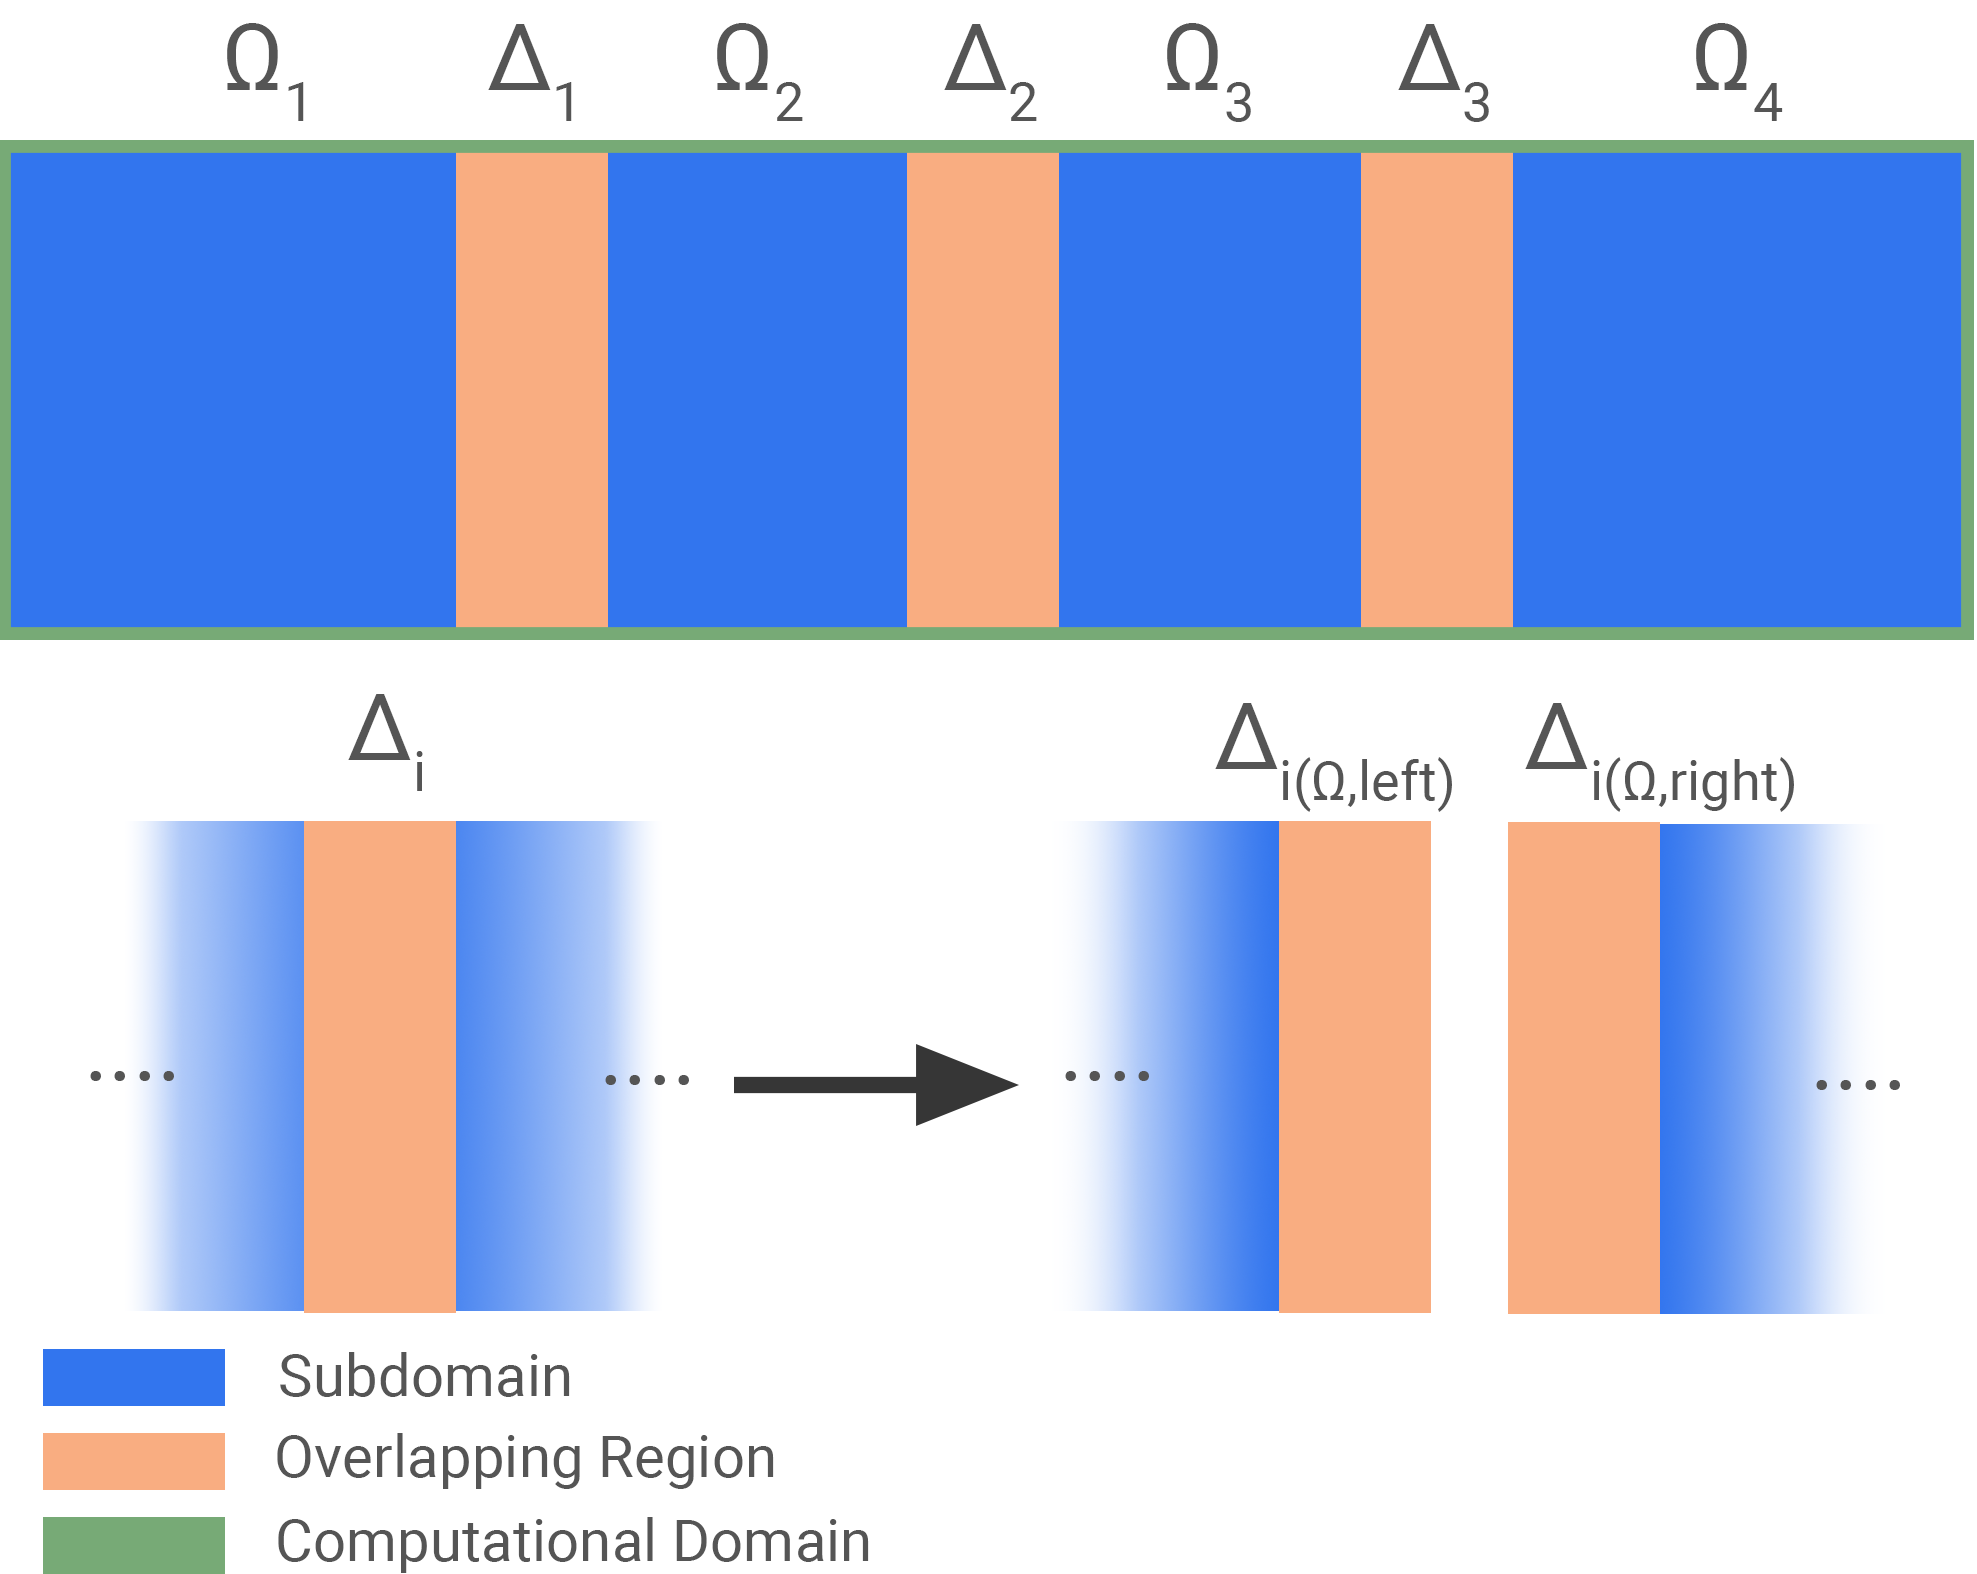
\includegraphics{images/subdomain_overlapping_region.png}
    \caption{Layout of Partitioned subdomains in the Computational Domain (top), Composition of an overlapping region (bottom)}
    \label{fig:subdomains}
\end{figure}

The process of convergence in Schwarz Alternating Method is done in each subdomain at least once because if a certain subdomain is in the middle, meaning they have two overlapping regions, the convergence process is done on each overlapping region. For example, in Figure \ref{fig:subdomains}, the computational domain is partitioned into 4 subdomains ($\Omega_1$ - $\Omega_4$) and thus it has three overlapping regions ($\Delta_1$ - $\Delta_3$). This shows that $\Omega_2$ and $\Omega_3$ have two overlapping regions ($\Delta_{i(\Omega, left)}$ and $\Delta_{i(\Omega, right)}$ in Fig. \ref{fig:subdomains}). In each subdomain, there will always be at least one overlapping region (in the case of a subdomain at the edge of the computational domain) and two overlapping region for the left and right adjacent subdomains (for the subdomains positioned in the middle of the computational domain).

\begin{algorithm}
	\caption{Data Transfer in each subdomain for convergence checking} 
	\begin{algorithmic}[1]
		\For {$subdomain\,\,\, i=1,2,\ldots n-1$}
			\State Transfer $\Delta_{i(\Omega _{i+1})}$ data to $\Omega_{i}$
			\State Process convergence by using $\Delta_{i(\Omega _{i})}$ and $\Delta_{i(\Omega _{i+1})}$ in $\Omega_i$
		\EndFor
	\end{algorithmic} 
\end{algorithm}

The decided data transfer flow is that the convergence on $\Delta_1$ is done on $\Omega_1$ node, meaning the data from $\Delta_1$ of $\Omega_2$ is transferred to $\Omega_1$ so that the convergence is processed. This pattern is repeated such that the left subdomain of the overlapping region is the node that will process the convergence. This means that the rightmost subdomain will not process the convergence on their connected overlapping region.\\


\subsection{Post-Processing}

After the simulation run has finished, the post-processing stage will begin and consolidate the simulation results and start data visualization. In the serial configuration, the process is simple: the simulation results are saved into several output files in .csv format. The format of the output file is shown below:

\begin{table}[H]
\caption{Format of Output File\label{tab:output_file}}

\centering{}%
\begin{tabular}{|c||c c c c c| }
\hline 
&\textbf{Column 0} & \textbf{Column 1} & \textbf{Column 2} & \textbf{.....} & \textbf{Column $N_z$}\tabularnewline
\hline 
\hline 
\textbf{Row 0} & $X|^{k=0}_{t=0}$ & $X|^{k=1}_{t=0}$ & $X|^{k=2}_{t=0}$ & ..... & $X|^{k=N_z}_{t=0}$ \tabularnewline
\textbf{Row 1} & $X|^{k=0}_{t=1}$ & $X|^{k=1}_{t=1}$ & $X|^{k=2}_{t=1}$ & ..... & $X|^{k=N_z}_{t=1}$ \tabularnewline
\textbf{Row 2} & $X|^{k=0}_{t=2}$ & $X|^{k=1}_{t=2}$ & $X|^{k=2}_{t=2}$ & ..... & $X|^{k=N_z}_{t=2}$ \tabularnewline
\textbf{.} & . & . & . & . & . \tabularnewline
\textbf{.} & . & . & . & . & .  \tabularnewline
\textbf{.} & . & . & . & . & .  \tabularnewline
\textbf{.} & . & . & . & . & .  \tabularnewline
\textbf{Row $N_t$} & $X|^{k=0}_{t=N_t}$ & $X|^{k=1}_{t=N_t}$ & $X|^{k=N_t}_{t=2}$ & ..... & $X|^{k=N_z}_{t=N_t}$  \tabularnewline

\hline 
\end{tabular}
\end{table}

This format will be applied to the electric field, magnetic field, reflectance, and transmittance that will be saved in csv files. Each row in the csv file correspond to an iteration up to the last iteration $N_t$ while the columns indicate the cell in the computational domain from k=0 to $k=N_z$.

In parallel configuration, the process is similar to the serial configuration but there is an extra initial step where the data from the different subdomains are compiled to create the solution for the whole computational domain. After that, the different simulation results are saved into csv files with formats similar to Table \ref{tab:output_file}.\\

\noindent
\textbf{Data Plots}

The simulation results will be visualised by plotting each iteration of the whole computational domain. Two plots will be created: 
\begin{enumerate}
    \item Superimposed plots of the electric and magnetic fields; and
    \item Superimposed plots of reflectance, transmittance, and the sum of the previous two parameters
\end{enumerate}
These plots are then compiled to create a video file to make the visualization of the FDTD simulation better to see the propagation of the plane waves.

To facilitate the creation of a video from a set of images, the filename format of the images will be: ``\textbf{[parameter]\_image\_[iteration].jpeg}". The format specifies that [parameter] is the simulation parameters that are plotted, in this project there will only be two cases: (1) \textbf{EyHx} or (2) \textbf{TrRf} where they pertain to the electric field/magnetic field superimposition and reflectance/transmittance plots respectively.

The ffmpeg library is used to create a video from a set of images \cite{FfmpegDocs}. The bash command for the creation of a video from set of images is shown below:\\

\textit{ffmpeg -f image2 -framerate 200 -i [parameter]\_images\_\%07d.jpeg -s [Width]x[Height] [output name].mp4}\\

The bash command above creates a video from a set of images that are created by the program in .mp4 format. In this way, the behavior of the electric and magnetic fields inside the computational domain is easily visualize and data can be compressed. 

\section{Testing}

The testing part of the methodology discusses how the testing will be done on each machine configuration and the different variables that will be changed in the configuration. The simulation accuracy of the project will also be discussed as well as the measurement of different metrics of performance for the parallel configuration.\\


\subsection{Testing Configuration}

The simulations done in this project are divided in two parts: (1) Serial configuration and (2) Parallel Configuration. The first part, is the reference simulation where the FDTD algorithm (see subsection \ref{subsec:fdtd_method}) is done without any parallelization schemes. This is used as a reference so that the parallel-FDTD algorithm (see subsection \ref{subsec:fdtd_schwarz_disc}) can be compared to a standard FDTD simulation to determine the accuracy of the parallel-FDTD algorithm. The second part is the simulations for the parallel-FDTD algorithm in which the parallelization scheme is used. In both parts, simulations in the chosen open source FDTD tools will be done to determine the accuracy of the project's algorithm with other tools. 

In these simulations, there will be a default configuration of simulation parameters (in each machine configuration) where the independent variables will be changed one at a time to find out what parameters affect the performance and accuracy of the algorithm.

\begin{table}[H]
\caption{Default machine configuration\label{tab:def_config_table}}

\centering{}%
\begin{tabular}{|c|c c| }
\hline 
\textbf{Machine Configuration} & \textbf{Independent Variables} & \textbf{ Default Value} \tabularnewline
\hline 
\hline 
& Total Grid Size & $3(d_{total})$ \tabularnewline
& Simulation Time & $100\tau$ \tabularnewline
Serial Configuration & Model Complexity & Plane wave propagation in different media \tabularnewline
& Source Excitation & Gaussian Pulse \tabularnewline

\hline
\hline

& Total Grid Size & $3(d_{total})$ \tabularnewline
& Simulation Time & $100\tau$ \tabularnewline
Parallel Configuration & Model Complexity & Plane wave propagation in different media \tabularnewline
& Source Excitation & Gaussian Pulse \tabularnewline
& No. of subdomain & $2^3$ \tabularnewline
& Size of overlapping region & $30\%(d_{subdomain})$ \tabularnewline
\hline

\end{tabular}
\end{table}

In table \ref{tab:def_config_table}, the values that will be used in each configuration by default (before any independent variable are changed) is shown. Each independent variable that will be tested are explained below:

\begin{itemize}
    \item \textbf{Total Grid Size} - is the size of the whole computational domain (see Figure \ref{fig:layout_comp_domain}) and the value is dependent on the size of the simulation model used (in this case 3x the size of the simulation model). This means that the spacer region must be increased such that the total size of the computational domain is 3x the size of the simulation model.
    \item \textbf{Simulation Time} - is the time in which the FDTD time loop will iterate. This is not the actual run time of the simulation but the set simulation time ($t_{sim}$) in the input file. This value is dependent on $\tau$, which is based on the maximum frequency of interest in the source excitation (see equations \ref{eq:gauss_tau} and \ref{eq:sin_tau}) and in this case it is 100x the value of $\tau$.
    \item \textbf{Model Complexity} - is the simulation model that will be used in the simulation run. The selected default simulation model is the Plane wave propagation in different media (Figure \ref{fig:1st_model}).
    \item \textbf{Source Excitation} - is the type of EM source that will be used in the simulations. The selected default source excitation is Gaussian pulse (equation \ref{eq:gauss_orig}).
    \item \textbf{No. of subdomain} - is the number of subdomains that will be used in the parallel configuration. The selected default value is $2^3\,=\,8$ subdomains.
    \item \textbf{Size of overlapping region} - is the portion of the subdomain that \textit{overlaps} with the other subdomain. This value is dependent on the size of the subdomain (since each subdomain has equal size) and in this case it is 30\% of the size of each subdomain.
\end{itemize}


\begin{table}[H]
\caption{List of independent and dependent variables for each machine configuration\label{tab:ind_dep_table}}

\centering{}%
\begin{tabular}{|c|c c| }
\hline 
\textbf{Machine Configuration} & \textbf{Independent Variables} & \textbf{Dependent Variables} \tabularnewline
\hline 
\hline 
& Total Grid Size & Speedup \tabularnewline
& Simulation Time & Efficiency \tabularnewline
Serial Configuration & Model Complexity & Simulation Runtime \tabularnewline
& Source Excitation  & Percent Error \tabularnewline

\hline
\hline

& Total Grid Size & Speedup \tabularnewline
& Simulation Time & Efficiency \tabularnewline
Parallel Configuration & Model Complexity & Simulation Runtime \tabularnewline
& No. of subdomain & Percent Error \tabularnewline
& Size of overlapping region & Convergence Time \tabularnewline
& Source Excitation & \tabularnewline
\hline

\end{tabular}
\end{table}

Table \ref{tab:ind_dep_table} shows the different independent and dependent variables that will be used in the project. The independent variables are the parameters that will be varied one at a time (while using the default configuration for the other parameters) in each simulation run while the dependent variables are the metrics and measurements parameters that will indicate about the performance of the simulator as well its accuracy.\\

\noindent
\subsection{Simulation Accuracy}

In this part, the accuracy of the simulation with regards to each configuration as well as to other simulation results from open source tools will be discussed.\\

\noindent
\textbf{Convergence Condition in Schwarz Algorithm}

The convergence condition of each subdomain in Schwarz Alternating Algorithm is one of the most important aspect of that method because this convergence condition determines if the algorithm will repeat to the starting point or finish. An important parameter of the convergence condition is $\epsilon_{tol}$ (see equation \ref{eq:converge_cond}) or the error tolerance of the algorithm.

The error tolerance $\epsilon_{machine}$ used in the convergence of Schwarz Alternating method was selected based on \cite{Mota2017} where it is also referred as machine epsilon  and defined as  ``Difference between 1 and the least value greater than 1 that is representable" \cite{PythonDocs}. This definition of the error tolerance can give enough accuracy between the values in the serial configuration and parallel configuration such that when the algorithm achieve convergence, there will be no discrepancy between the serial configuration and parallel configuration.
%https://docs.python.org/3/library/sys.html 

In order to get the value of the machine epsilon, there are built-in libraries for C++ and Python that can be used in order to set the error tolerance without setting a constant in the code (since it might be machine dependent).For C++, the standard library (std) can be used by using the statement ``\textbf{std::numeric\_limits$<$double$>$::epsilon()}" \cite{CppDocs}. In Python, the \textit{sys library} is the library that can be used to get the machine epsilon, using the statement ``\textbf{sys.float\_info.epsilon}" \cite{PythonDocs}.\\

\noindent
\textbf{Error Analysis}

The accuracy of simulation results of the parallel configuration is compared to the serial configuration and both the serial and parallel configuration will be compared to the results of the simulation from open source FDTD tools. To measure the difference in results, percent error is used shown below:

\begin{align}
    Percent\,error\,=\,|\frac{X_{reference} - X_{simulation}}{X_{reference}}|\times 100\%\label{eq:percent_error}
\end{align}

As shown in equation \ref{eq:percent_error}, the formula used is relative error that is converted into percentage. In the context of this project, the electric and magnetic field is the parameters that will be compared because these are the main products of the FDTD algorithm. The equations below show the specific equations that will be used for each configuration.

\begin{align}
    &E_{\%_{error}}\,=\,|\frac{E_{serial/other} \,-\,E_{parallel/serial}}{E_{serial/other}}|\times 100\% \label{eq:E_percent_error}\\
    &\tilde{H}_{\%_{error}}\,=\,|\frac{\tilde{H}_{serial/other} \,-\,\tilde{H}_{parallel/serial}}{\tilde{H}_{serial/other}}|\times 100\% \label{eq:H_percent_error}
\end{align}

The percent error for both the electric and magnetic fields are computed depending on the configurations. In the case of serial configuration, the reference simulation results is the results from the open source FDTD tools. In parallel configuration, the reference simulation results are the simulation results from the serial configuration and the open source FDTD tools. Another aspect that can be done to check the accuracy of the results is to superimpose the plots of each simulation results to see how close the results are with each other and to determine if some parts in the computational domain have a higher error or lesser error.\\

\noindent
\subsection{Performance Analysis}

This part discusses on how the performance of the parallel configuration is measured using the \textbf{speedup} and \textbf{efficiency} metrics.

\subsubsection{Speedup}\label{subsub:SP}

Most researches \cite{Ramadan2017, Zheng2016, Lin2013} in parallel computing use relative speedup in measuring the effect of increasing the number of subdomain in a simulation runtime. The equation for relative speedup is shown below:

\begin{align}
    S_P\,=\,\frac{T(1)}{T(P)}
    \label{eq:speedup}
\end{align}

In \cite{Hoffmann1993}, the relative speedup is defined as the ratio of the successful runtime of an algorithm using one processor and the successful runtime of the same algorithm using P number of processors. 

In the metric of speedup, since each subdomain corresponds to a node/processor, the expected result is that the speedup of the configuration will be better as the number of subdomains increases because each subdomain will have smaller area to compute when the subdomains have increased in number. Also, the serial configuration will be used as a reference value since the speedup of the serial configuration is 1. Based on equation \ref{eq:speedup}
, as the number of subdomains approach infinity, the speedup will approach 0. This suggest that a smaller speedup value results in better performance. This metric, however is not the only measurement of performance that is needed to be considered so another parameter, efficiency is discussed next.\\


\subsubsection{Efficiency}

Same as in subsubsection \ref{subsub:SP}, most researches in parallel FDTD research uses another metric for measuring the efficiency of the algorithm. This metric is called \textbf{relative parallel efficiency}.

\begin{align}
    E(P)\,=\,\frac{S_P}{P}
    \label{eq:efficiency}
\end{align}

Relative parallel efficiency is defined in \cite{Hoffmann1993} as the ratio between the speedup (equation \ref{eq:speedup}) and the number of processors P. This metric is useful for measuring the performance of an algorithm on how efficient it can use each processor.

The efficiency (equation \ref{eq:efficiency} )
can be used to describe on how efficient the algorithm in utilizing the processors used in the algorithm. This is because as the number of processors decrease, the efficiency increases while the speedup is directly proportional to the efficiency. The ideal efficiency value is 0 or when the speedup reaches 0 and the number of processors used is 1. This metric, along with speedup can be used to describe the performance of the parallel configuration of the project.\\

\noindent
\textbf{Simulation Runtime and Convergence Time}

The last two parameter that measures the total simulation runtime and convergence time in the Schwarz Alternating Method. These parameters are also important to measure in the testing part of the methodology because they can give some description on how long the simulation will run. The convergence time will always be less than the total simulation runtime because in every simulation runtime, there will be multiple convergence time because the Schwarz Alternating Method is done on every subdomain. 

The simulation runtime is the total amount of time (in seconds) on how long the simulation runs starting from the pre-processing stage to the post-processing stage. Convergence time, on the other hand is the amount of time from the start of an instance of Schwarz Alteranting Method to the end when all subdomain have converged.

These parameters can help in identifying what independnet variables have significant effect of the runtime of the simulations.

\noindent
\subsection{Data Visualization}

Since in the testing, there will be numerous simulation results from numerous simulation runs, data visualization is necessary to see the different trends from the data. The superimposition of different plots on each other can help in determining the patterns that emerge in the data. Tabulating the metrics can also be used to compare the values closely and make sure that the analysis can be done on the data properly. These methods will be used after the simulation results are completed in each configuration. 


\cleardoublepage{}

\chapter{Preliminary Findings\label{cha:Prelims}}

In this part, the initial simulation results from our current implementation of 1D FDTD is presented. The FDTD algorithm used in this part is similar to subsection \ref{subsec:fdtd_method}. The difference is on the boundary condition used which is only the Dirichlet Boundary condition, which the boundary at the end of the computational domain acts like a perfect electric conductor and perfect magnetic conductor.

The simulation parameters used are $f_{MAX}\,=\,2.4 GHz$, Gaussian Pulse and No Source, Dirichlet Boundary condition, Perfectly Absorbing Boundary Condition (PABC), and the computational domain is composed of only  air or vacuum while the simulation model used is a single layer of glass ($\mu = \frac{3}{8}$, $\epsilon = 8$ ). The following figures are the simulation results when: (1) No source excitation, (2) Gaussian pulse using Hard source method, (3) Gaussian pulse using Soft source method, and (4) Gaussian pulse using Soft source with PABC.

\begin{figure}[H]
    \centering
    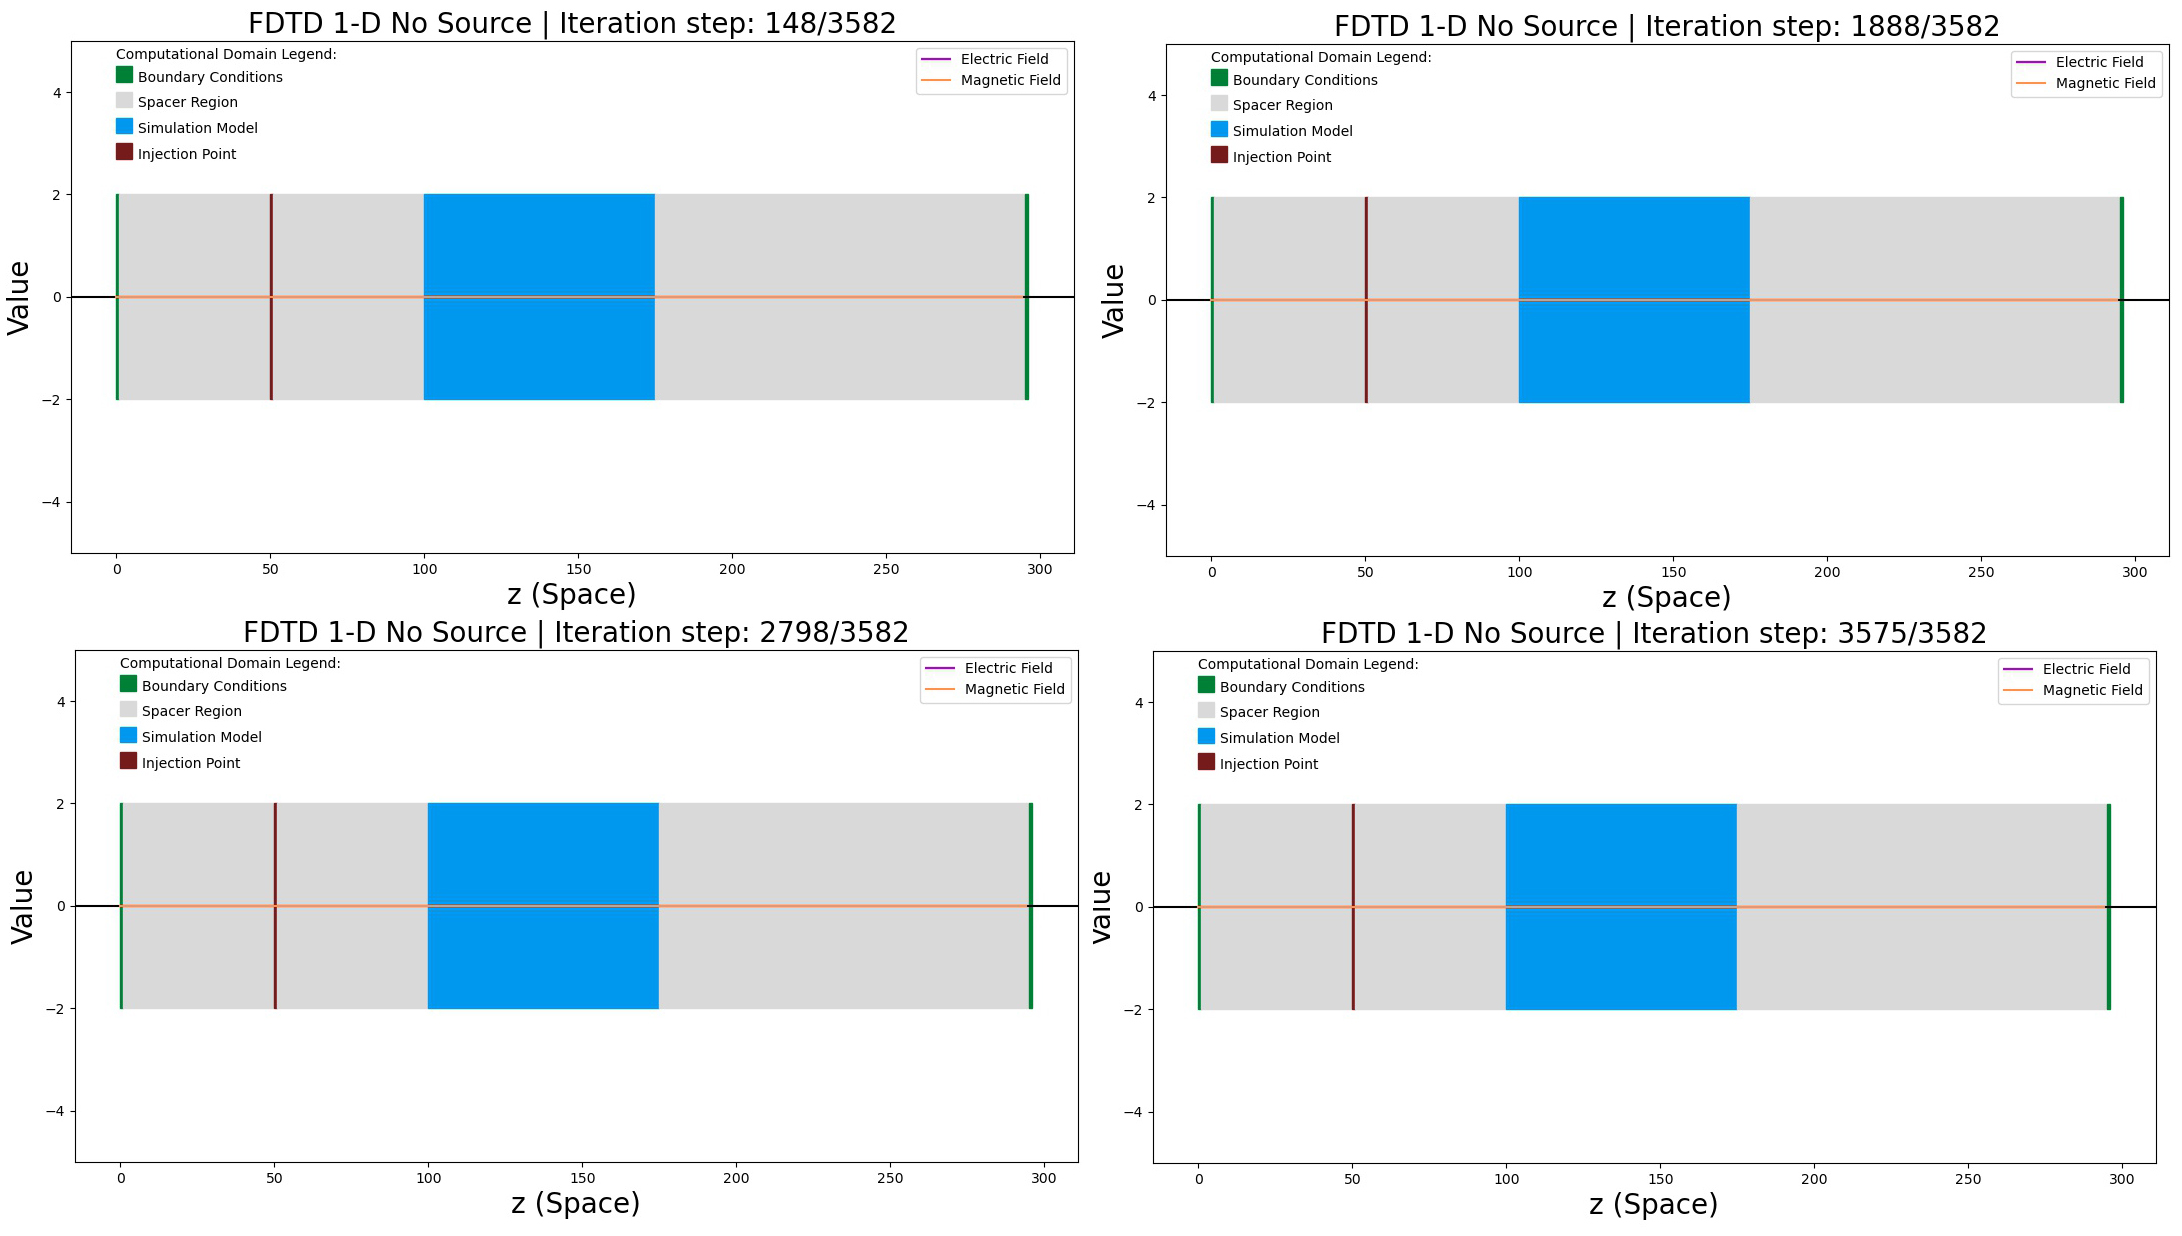
\includegraphics[width=\textwidth]{images/no_source_prelim.jpg}
    \caption{FDTD Simulation Results at different time step (No Source Excitation)}
    \label{fig:no_source_prelim}
\end{figure}

As shown in Figure \ref{fig:no_source_prelim}, the FDTD simulation shows that there is no change in the electric and magnetic field. This means that the simulation is stable enough and does not show any errors when there is no source excitation. The results are expected since there is no outside EM source to excite the computational domain, there will be no change in the initial electric and magnetic field values.

\begin{figure}[H]
    \centering
    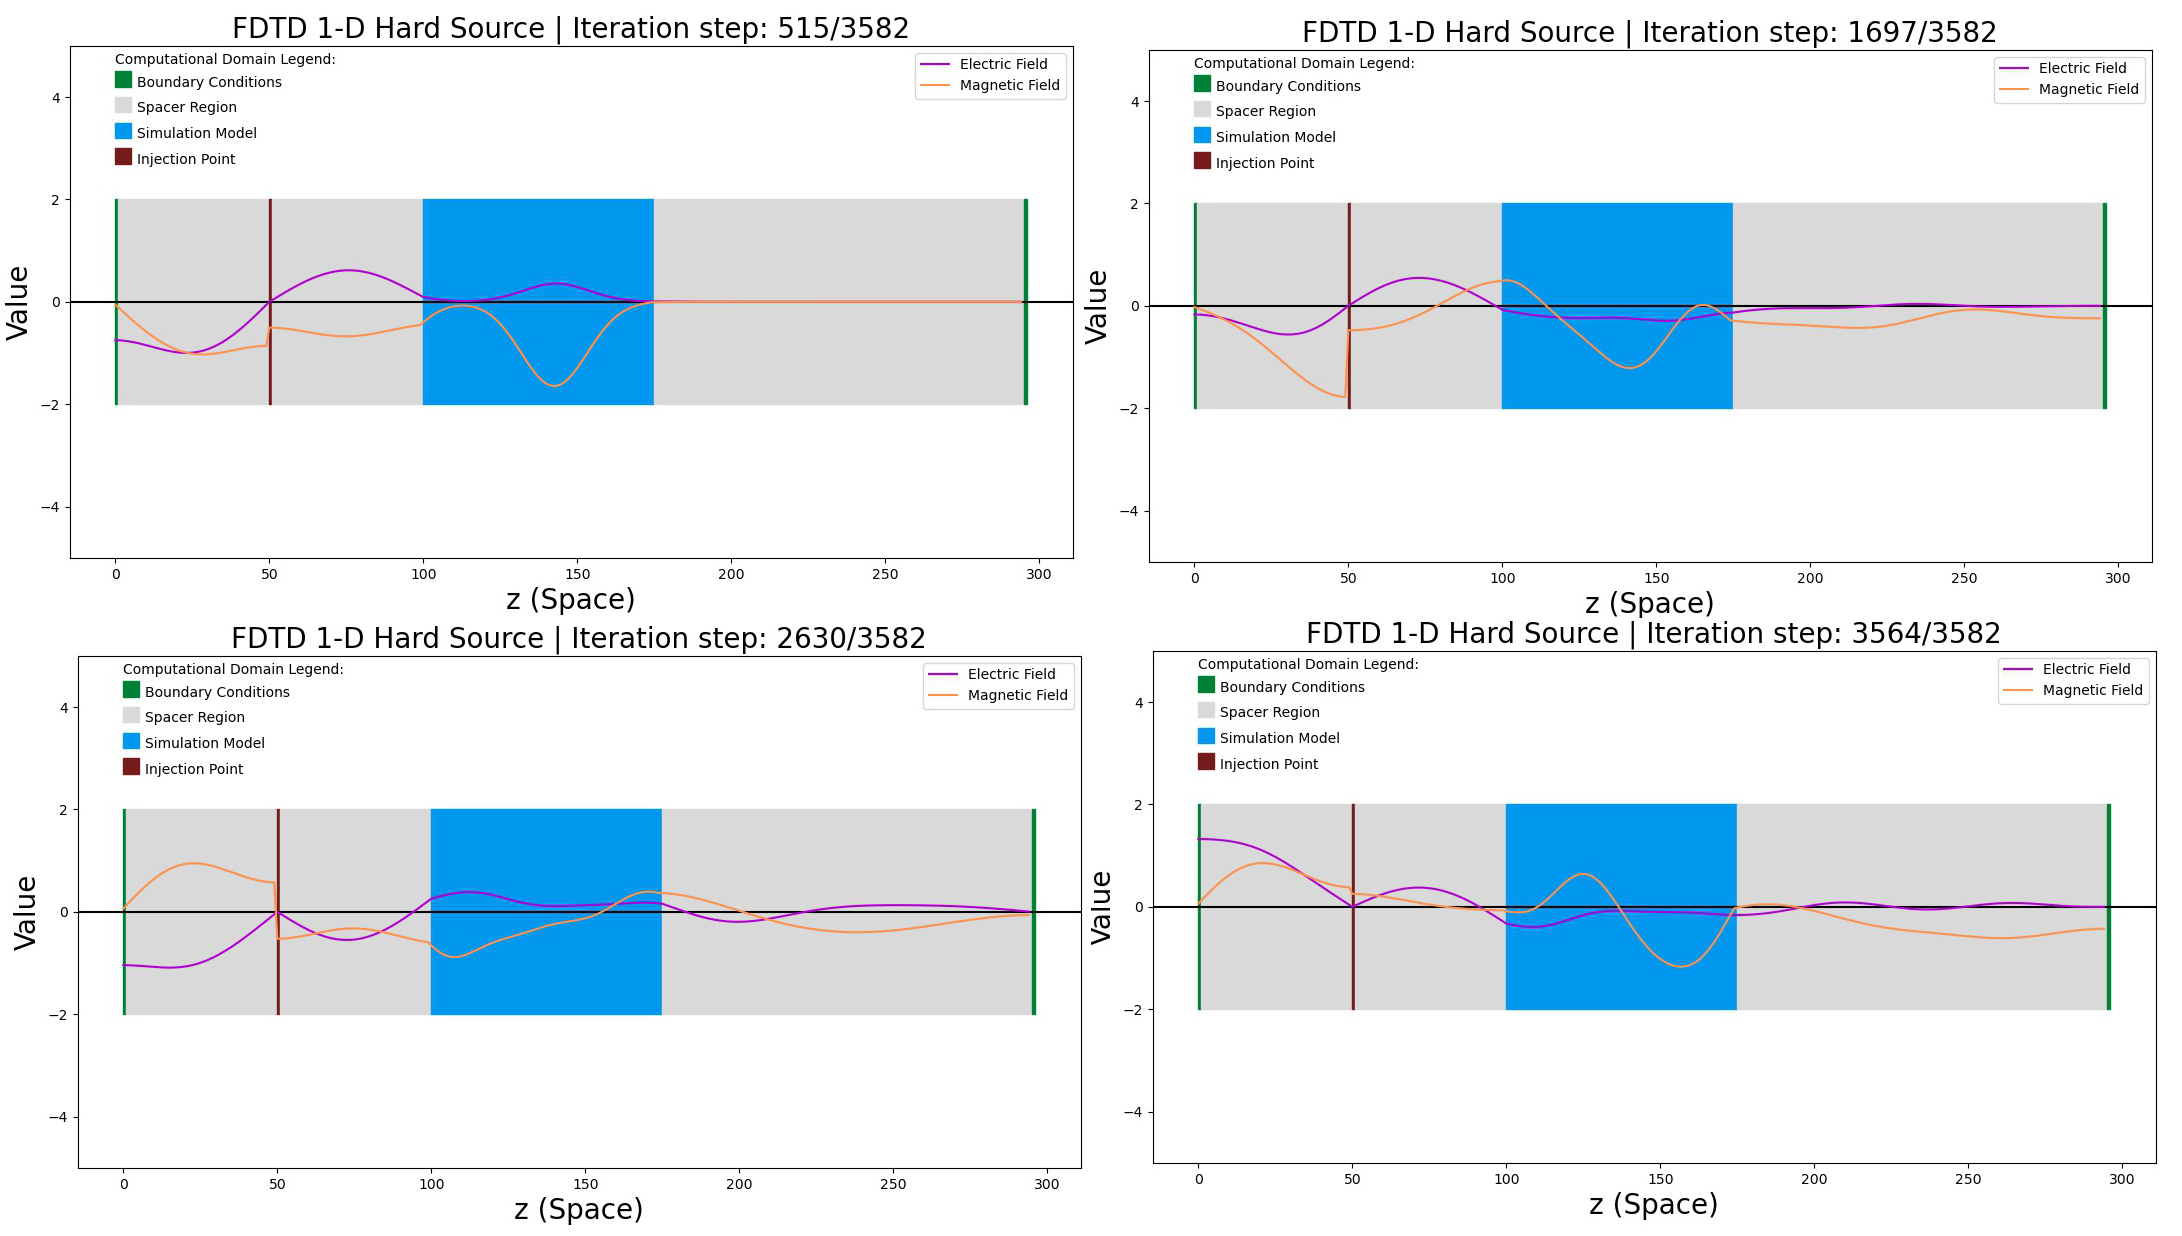
\includegraphics[width=\textwidth]{images/hard_source_prelim.jpg}
    \caption{FDTD Simulation Results at different time step (Gaussian Pulse in Hard Source Method)}
    \label{fig:hard_source_prelim}
\end{figure}

As shown in Figure \ref{fig:hard_source_prelim}, the FDTD simulation has injected the Gaussian Pulse in the center of the computational domain. Two pulses were produced (propagates to the left and right direction) and since the boundary condition used are Dirichlet Boundary conditions, the pulses bounces off of the boundaries and cannot propagate outside the computational domain. The injection point also acts like a wall between the two pulses so they cannot interact with each other. This is because Hard source method forces the injection by overwriting the field value at the injection point and disregards the previous value. Also, the fields are distorted (slower and change in shape) when it enters the glass material and reverts back to its original shape and speed after exiting the glass material. It  is also important to note that small reflections occur as the fields enter a change in material (when it enter or exit the glass).

\begin{figure}[H]
    \centering
    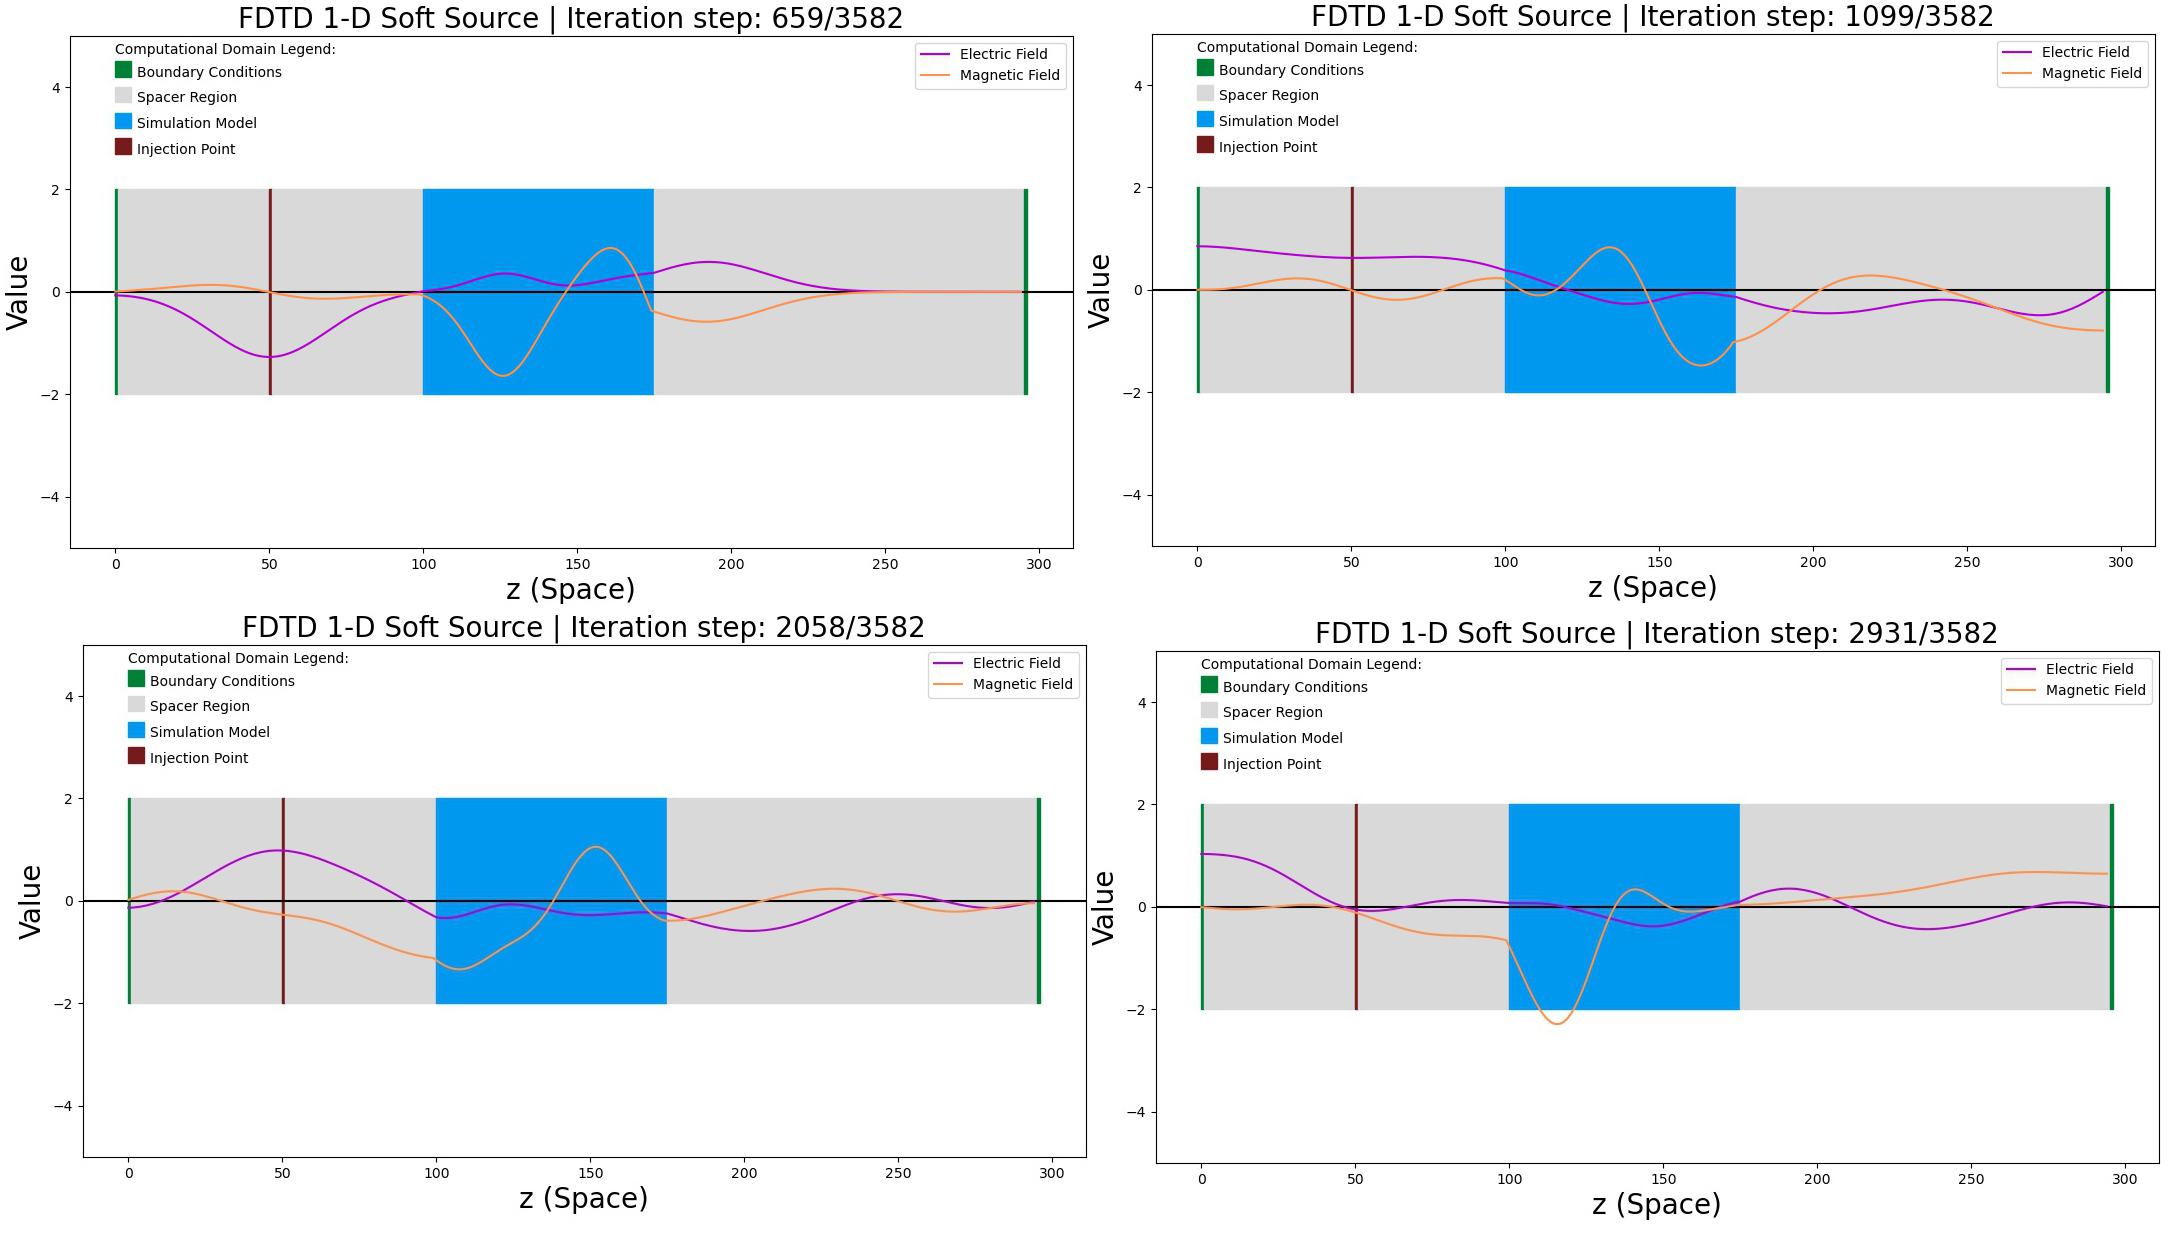
\includegraphics[width=\textwidth]{images/soft_source_prelim.jpg}
    \caption{FDTD Simulation Results at different time step (Gaussian Pulse in Soft Source Method)}
    \label{fig:soft_source_prelim}
\end{figure}

The next figure (Figure \ref{fig:soft_source_prelim}) shows the simulation results similar to the one in Figure \ref{fig:hard_source_prelim} but the method of excitation is soft source method where the value of the source at the injection point is added onto the previous value of the fields so that the two pulses can interact with each other. However, since the boundary conditions are Dirichlet and the material is lossless, the pulses will not fade but bounce around the computational domain until the simulation ends.

\begin{figure}[H]
    \centering
    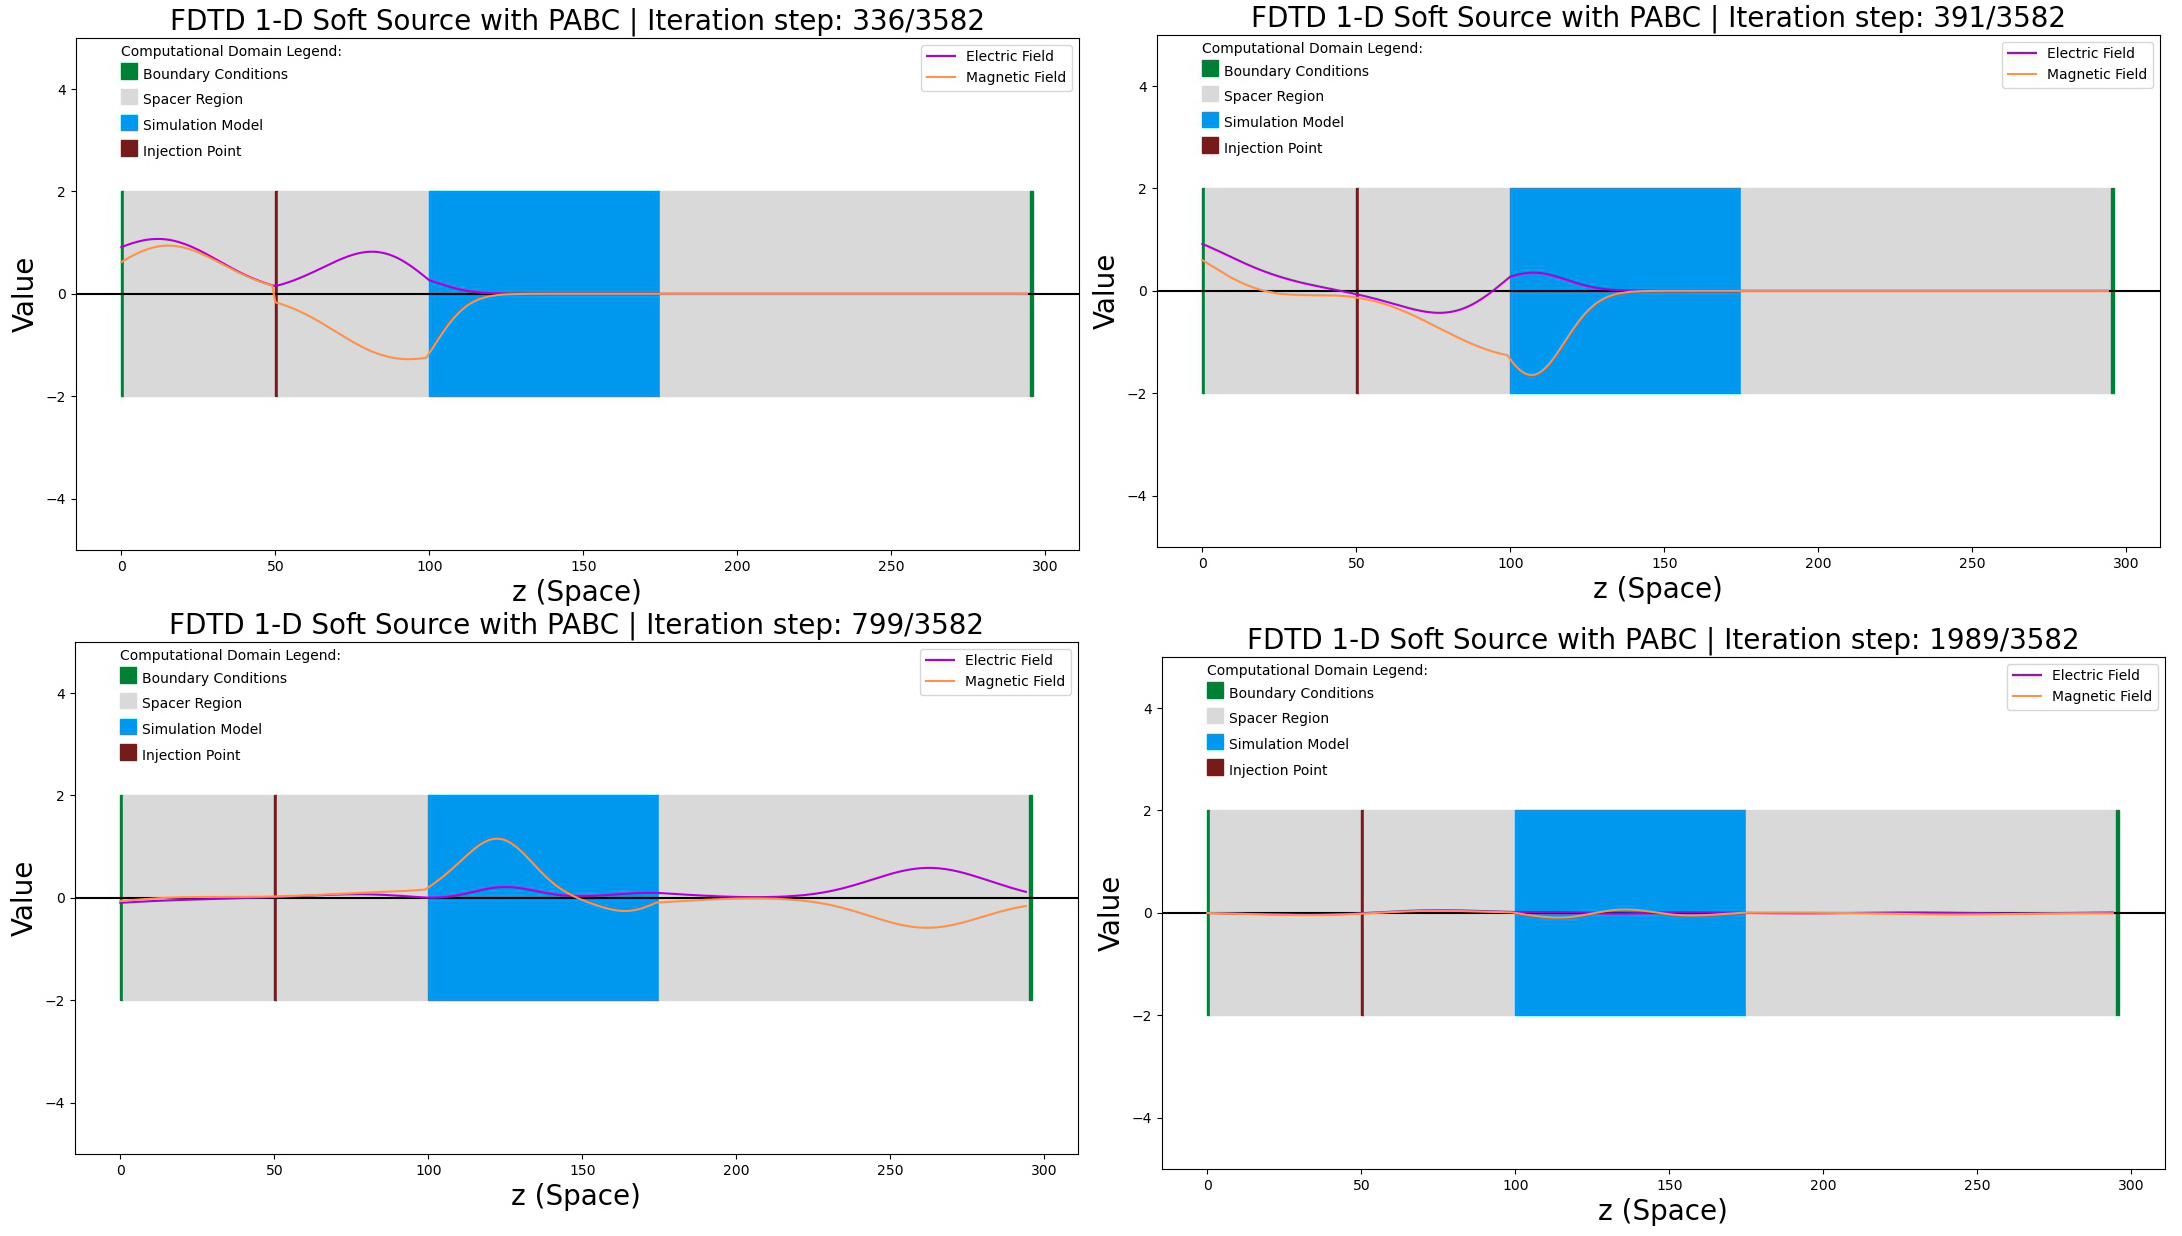
\includegraphics[width=\textwidth]{images/soft_source__pabc_prelim.jpg}
    \caption{FDTD Simulation Results at different time step (Gaussian Pulse in Soft Source Method and PABC)}
    \label{fig:soft_source_pabc_prelim}
\end{figure}

The last figure (Figure \ref{fig:soft_source_pabc_prelim}) shows similar results and observation as the previous figure (Fig. \ref{fig:soft_source_prelim}). The main difference is the boundary condition used which is PABC. The results show that the fields can now propagate outside of the computational domain as shown in the figure as the time step increase, there are fewer field values that change and it becomes smaller. However, it is not a perfect boundary condition as since it is also noticed that small reflections (similar to what happens when field enter or exit a new material) occur as shown in time step 799 when the reflection of the fields enter the glass material.

\cleardoublepage{}

\chapter{Results and Discussion}

\section{Problems Encountered}
In this section, problems that were encountered during the implementation of the project will be presented. Actions done to solve these challenges will also be included in this section. 

\subsection{Ringing in the computational domain when source is sinusoidal}
When first implementing the 1-D FDTD algorithm, some erratic behavior was observed when the waves are propagating across the computational domain. This happens when the source type is sinusoidal and the boundary conditions is PABC. 

The problem was caused by an error in the initialization of two of the vectors used to store the field values. There was a misuse of the \texttt{range()} function of the Xtensor library. 

\subsection{Unwanted energy propagating in the wrong direction}
It has been observed that some energy was propagating to the left of the source injection point. This is unwanted behavior since the implementation of the source should be one-sided. The culprit of this problem was a mistype in the code --- the places of two variables in the code were unknowingly exchanged. 


\textbf{From Week 1 and 2}
\begin{enumerate}
    \item Ringing in the computational domain when source is sinusoidal
    \item PABC does not completely allow the pulse to propagate freely, some energy is still reflected back
\end{enumerate}

\textbf{From Week 3}

\section{Features}

\begin{enumerate}
    \item Boundary conditions - PABC and Dirichlet
    \item Sources - sinusoidal, Gaussian pulse, ****
    \item Excitation method - hard, soft, TF/SF
\end{enumerate}

\section{Code Dependencies/Libraries used}
\begin{enumerate}
    \item Xtensor library - useful for matrix oprations 
    \item Xtl - prerequisite of xtensor
    \item HighFive - used for plotting of results(??)
    \item plotly
    \item matplotlib
    
\end{enumerate}


\cleardoublepage{}

\chapter{Project Schedule and Deliverables\label{cha:Project-Sked}}

% For final project documentations, this chapter becomes the Conclusions
% and Recommendations chapter.

% For project proposals, end the documentation by presenting the project
% schedule and expected deliverables. This section should clearly describe
% the activities that will be done. Important milestones should be indicated
% in the schedule of activities. It should be as specific as possible. 


\section{Gantt Chart }

% This is a time table that clearly indicates the important milestones
% of the project. The schedule should be divided into weekly segments.
% The authors should make sure that the schedules are realistic. It
% is advised that the weekly tasks are as detailed as possible. 
The Gantt Chart for this project is shown in Figure 6.1. It is assumed that the project will run for twelve weeks. The chart is color-coded according to which proponent is responsible for a certain task. The blue-colored bars are assigned to Mr. Moyco, while the purple-colored bars are assigned to Mr. Alaan. The green-colored bars are assigned to both members of the team. 

%This gantt chart is primarily from 
%https://www.overleaf.com/project/60b9a2a51babf789b96d756d
%Colors for the gantt chart
\definecolor{marvin}{RGB}{111, 168, 220}
\definecolor{karlo}{RGB}{180, 167, 214}
\definecolor{both}{RGB}{106, 168, 79}

%16 week verson of gantt chart

%\begin{figure}[H]
%    \hskip-1.5cm
    %15
%    \resizebox{\textwidth}{!}{
%    \begin{ganttchart}[
%        canvas/.append style={fill=none, draw=black!5, line width=.5pt},
%        x unit = .75cm,
%        hgrid style/.style={draw=black!5, line width=.75pt},
%        vgrid={*1{draw=black!5, line width=.1pt}},
%        title/.style={draw=none, fill=none},
%        title label font=\bfseries\footnotesize,
%        title label node/.append style={below=5pt},
%        include title in canvas=false,
%        newline shortcut = false,
%        bar label font=\mdseries\small\color{black},
%        bar label node/.append style={align=right},
%        bar/.append style={draw=none, fill=black!63},
%        progress label text ={},
        %group progress label font=\bfseries\small,
%      ]{1}{16}
%        \sffamily
%        \gantttitle{WEEKS}{15}\ganttnewline
%        \gantttitlelist{1,...,16}{1}\ganttnewline
%        \ganttbar[progress=0,bar incomplete/.append style={fill=marvin}]{Implement a full-featured 1D FDTD in serial configuration}{1}{2}\ganttnewline
%        \ganttbar[progress=0,bar incomplete/.append style={fill=karlo}]{Implement Schwarz Alternating Method in code}{1}{2}\ganttnewline
%        \ganttbar[progress=0,bar incomplete/.append style={fill=both}]{Combine FDTD and Schwarz Alternating Method}{3}{3}\ganttnewline
%        \ganttbar[progress=0,bar incomplete/.append style={fill=both}]{Implement the combined FDTD-Schwarz Algorithm in parallel configuration}{4}{6}\ganttnewline
%        \ganttbar[progress=0,bar incomplete/.append style={fill=both}]{Implement the combined FDTD-Schwarz Algorithm in cloud configuration}{7}{7}\ganttnewline
%         \ganttbar[progress=0,bar incomplete/.append style={fill=both}]{Create the input/output handling of the system}{8}{8}\ganttnewline
%        \ganttbar[progress=0,bar incomplete/.append style={fill=marvin}]{Create a simulation model of a plane wave propagation in different media}{9}{9}\ganttnewline
%        \ganttbar[progress=0,bar incomplete/.append style={fill=karlo}]{Create a simulation model of bragg grating}{9}{9}\ganttnewline
%        \ganttbar[progress=0,bar incomplete/.append style={fill=both}]{Simulation results of FDTD Algorithm \\ in serial configuration with varying simulation parameter and model}{10}{11}\ganttnewline \ganttnewline
%        \ganttbar[progress=0,bar incomplete/.append style={fill=both}]{Simulation results of Combined FDTD-Schwarz Alternating Algorithm \\ in parallel configuration with varying simulation parameter and model}{12}{13}\ganttnewline \ganttnewline
%        \ganttbar[progress=0,bar incomplete/.append style={fill=both}]{
%        Simulation results of Combined FDTD-Schwarz Alternating Algorithm \\in cloud configuration with varying simulation parameter and models
%        }{14}{16}\ganttnewline \ganttnewline
%        \ganttbar[progress=0,bar incomplete/.append style={fill=both}]{Simulation results of open-source FDTD tools using \\ similar simulation parameters and models
%        }{10}{16}\ganttnewline \ganttnewline
%        \ganttbar[progress=0,bar incomplete/.append style={fill=both}]{Debugging}{10}{16}\ganttnewline
%        \ganttbar[progress=0,bar incomplete/.append style={fill=both}]{Comparison of the simulation results from different configurations}{10}{16}\ganttnewline
%        \ganttbar[progress=0,bar incomplete/.append style={fill=both}]{Documentation}{1}{16}
%    \end{ganttchart}}
%    \caption{Gantt chart of the Project Proposal 16 Weeks version}
%\end{figure}

\begin{figure}[H]
    \hskip-1.5cm
    %15
    \resizebox{\textwidth}{!}{
    \begin{ganttchart}[
        canvas/.append style={fill=none, draw=black!5, line width=.5pt},
        x unit = .75cm,
        hgrid style/.style={draw=black!5, line width=.75pt},
        vgrid={*1{draw=black!5, line width=.1pt}},
        title/.style={draw=none, fill=none},
        title label font=\bfseries\footnotesize,
        title label node/.append style={below=5pt},
        include title in canvas=false,
        newline shortcut = false,
        bar label font=\mdseries\small\color{black},
        bar label node/.append style={align=right},
        bar/.append style={draw=none, fill=black!63},
        progress label text ={},
        %group progress label font=\bfseries\small,
      ]{1}{12}
        \sffamily
        \gantttitle{WEEKS}{15}\ganttnewline
        \gantttitlelist{1,...,12}{1}\ganttnewline
        \ganttbar[progress=0,bar incomplete/.append style={fill=marvin}]{Implement a full-featured 1D FDTD in serial configuration}{1}{2}\ganttnewline
        \ganttbar[progress=0,bar incomplete/.append style={fill=karlo}]{Implement Schwarz Alternating Method in code}{1}{2}\ganttnewline
        \ganttbar[progress=0,bar incomplete/.append style={fill=both}]{Combine FDTD and Schwarz Alternating Method}{3}{3}\ganttnewline
        \ganttbar[progress=0,bar incomplete/.append style={fill=both}]{Implement the combined FDTD-Schwarz Algorithm in parallel configuration}{4}{6}\ganttnewline
        \ganttbar[progress=0,bar incomplete/.append style={fill=both}]{Simulation results of open-source FDTD tools using \\ similar simulation parameters and models
        }{1}{6}\ganttnewline \ganttnewline
         \ganttbar[progress=0,bar incomplete/.append style={fill=karlo}]{Create a simulation models for the system}{7}{7}\ganttnewline
        \ganttbar[progress=0,bar incomplete/.append style={fill=marvin}]{Create the input/output handling of the system}{7}{7}\ganttnewline
        \ganttbar[progress=0,bar incomplete/.append style={fill=both}]{Simulation results of FDTD Algorithm \\ in serial configuration with varying simulation parameter and model}{8}{9}\ganttnewline \ganttnewline
        
        \ganttbar[progress=0,bar incomplete/.append style={fill=both}]{Simulation results of Combined FDTD-Schwarz Alternating Algorithm \\ in parallel configuration with varying simulation parameter and model}{10}{12}\ganttnewline \ganttnewline
        \ganttbar[progress=0,bar incomplete/.append style={fill=both}]{Debugging}{8}{12}\ganttnewline
        \ganttbar[progress=0,bar incomplete/.append style={fill=both}]{Comparison and analysis of the simulation results from different configurations}{8}{12}\ganttnewline
        \ganttbar[progress=0,bar incomplete/.append style={fill=both}]{Documentation}{1}{12}
    \end{ganttchart}}
    \caption{Gantt chart of the Project Proposal}
\end{figure}



\section{Halfway-point Deliverables}

% This section should clearly point out and describe the expected outputs
% at halfway-point. If the project will be done by a group, the deliverables
% of each group member shall be clearly and specifically stated. 
The following list shows the expected outputs of the group at the half-way point of the project. For this project, the proponents deemed the half-way point to be after the third week of the entire project duration. 

\begin{enumerate}
    \item Serial FDTD with features
    \item Schwarz Alternating Method Code
    \item Combination of the two algorithms implemented in series
\end{enumerate}

Item 1 is assigned to Mr. Moyco, while item 2 is assigned to Mr. Alaan. Item 3 is assigned to both members of the team. 
 
\section{Final Deliverables}

% This section should clearly point out the final deliverables. If the
% project will be done by a group, the deliverables of each group member
% shall be clearly and specifically stated.

The following list shows the expected outputs of the group at the end of the project. 

\begin{enumerate}
    \item Implementation of the codes in parallel configuration
    \item Comparison of the simulation results of three configurations
    \item Documentation 
\end{enumerate}

All of the tasks listed above will be worked on by both members of the team. 

\cleardoublepage{}

\bibliographystyle{unsrt}
%\nocite{*}
%The references are currently stored in Mendeley, will be importing the bibtex to overleaf in the following days
\bibliography{eee190_bibliography.bib}
\cleardoublepage{}

%\appendix

%\chapter{Appendices}

%If there is only one appendix, it shall be labeled \textquotedblleft Appendix:\textquotedblright{}
%and the appendix title. If there are more than one appendices, they
%shall be labeled \textquotedblleft Appendix A: {[}title{]}\textquotedblright ,
%\textquotedblleft Appendix B: {[}title{]}\textquotedblright , etc.
%For software projects, appendices may include program listings, screen
%shots, and sample input and output files. For hardware projects, appendices
%may include printed circuit board layouts and geometric design layouts.
%Other possible appendices include user manuals (created by the author
%for the project), long mathematical proofs, and reviews of basic concepts.

%You can insert appendices through the \textbf{Document \textgreater{}
%Start Appendix Here} option. The appendix should start after the bibiliography
%section of the main document. Appendices can also have chapters and
%sections. \LyX{} automatically lists the appendices alphabetically.

%\cleardoublepage{}

%\chapter{Formatting Tips}

%\section{Inserting Chapters}

%On the upper left dropdown menu of the \LyX{} window, select \textit{Chapter}.
%You can then type the chapter title that you want. Pressing Enter
%will revert the format to \textit{Standard}, where the content can
%now be placed. Chapters are numbered and placed on the \textit{Table
%of Contents} automatically.

%\section{Inserting Sections}

%On the same dropdown menu where you insert a chapter, select \textit{Sections}.
%The sections under the chapter are automatically numbered accordingly.
%These also appear in the generated \textit{Table of Contents}.

%\subsection{Subsections}

%You can also add subsections and subsubsections. However, use them
%sparingly, especially the latter.

%\section{Inserting Labels}

%On the chapter/section/image/table that you want to reference, click
%\textbf{Insert \textgreater{} Label}. You can use the default label
%that \LyX{} generates for you. To 'call' it anywhere in your document,
%click the \textbf{Insert \textgreater{} Cross-reference}. This provides
%an efficient way of pointing out figure/table and chapter/section
%numbers, without the need to type out explicitly what the numbers
%are in the document.

%\section{Inserting Floats}

%Figures and tables shall be included in the body of the documentation
%to illustrate or clarify the accompanying text. Thus, figures and
%tables must be referenced in the text in order for them to be meaningful.
%By convention, figure names should be placed below the image, while
%table names should be placed on top of the table. 

%Moreover, figures or tables should not appear in the document before
%they are mentioned in the text. By default, \LyX{} does not follow
%this rule and places images or tables near, but not exactly after,
%the text referencing it. You can force the rule by right-clicking
%on the \textit{float:Figure} label in the \LyX{} editor and going to
%\textit{Settings}. In the window that appears, shown in Figure \ref{fig:Forcing-float-placement},
%uncheck \textit{Use default placement} and check \textit{Here definitely}
%instead.

%\begin{figure}[H]
%\begin{centering}
%
\includegraphics[width=0.5\columnwidth]{images/CMOS_or_nor.eps} 
%\par\end{centering}
%\caption{Forcing float placement\label{fig:Forcing-float-placement}}

%\end{figure}


%\subsection{Inserting Images}

%Place your cursor on the area where you want to insert the image.
%Select \textbf{Insert \textgreater{} Float \textgreater{} Figure}.
%Insert the actual image by selecting \textbf{Insert \textgreater{}
%Graphics}. It is a recommended practice that all images should be
%placed on a single folder on the same directory of this \LyX{} document
%template.

%You can also center the image by putting first your cursor on the
%side of the image that you want to center. Right click then select
%\textit{Paragraph Settings}. Finally, select the \textit{Center} button. 

%You can scale the images inside the document by clicking on the image.
%As shown in Figure \ref{fig:LyX-Graphics-options}, images can be
%scaled relative to the column width. For two column document formats,
%scale the image relative to the text width.

%\begin{figure}[H]
%\begin{centering}
%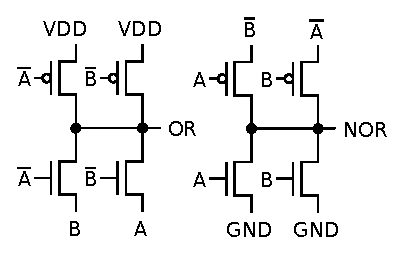
\includegraphics[width=0.6\columnwidth]{images/DPL_or.eps}
%\par\end{centering}
%\caption{\protect\LyX{} Graphics options\label{fig:LyX-Graphics-options}}

%\end{figure}

%As shown in Figure \ref{fig:Subfloat-Sample}, we can also insert
%floats within the float. To put the subfloat to the document center,
%click on the side of the \textit{subfloat: Figure} field, instead
%of the image within the subfloat, and then access the \textit{Paragraph
%Settings} as described in the previous steps. 

%\begin{figure}[H]
%\begin{centering}
%\subfloat[Subfloat A]{\begin{centering}
%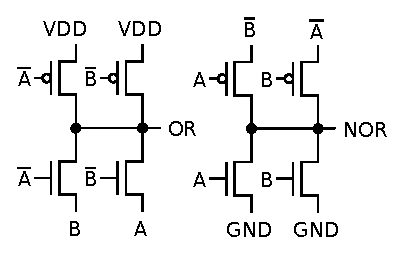
\includegraphics[width=0.8\columnwidth]{images/DPL_or.eps}
%\par\end{centering}
%}
%\par\end{centering}
%\begin{centering}
%\subfloat[Subfloat B]{\begin{centering}
%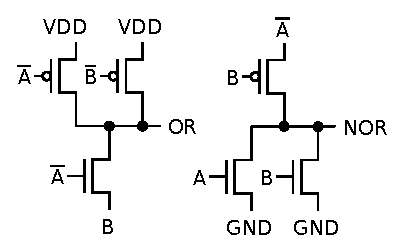
\includegraphics[width=0.8\columnwidth]{images/DVL_or.eps}
%\par\end{centering}
%}
%\par\end{centering}
%\caption{Subfloat %Sample\label{fig:Subfloat-Sample}}
%\end{figure}

%You may also put multiple figures in one line using the tabular inside a figure. You will have to manually add the subfigure label though when referencing, as in Figure \ref{fig:multi-fig}(a) shows ABC while Figure \ref{fig:multi-fig}(b) is for XYZ.

%\begin{figure*}[t] %t means top, b for bottom, h for here
%\centering
%\begin{tabular}{ c c c } 
% 
\includegraphics[width=5cm,keepaspectratio]{images/CMOS_or_nor.eps} & 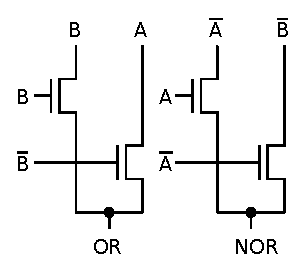
\includegraphics[width=5cm,keepaspectratio]{images/CPL_or.eps} & 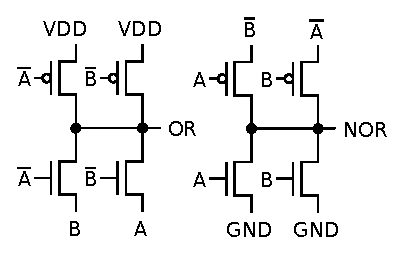
\includegraphics[width=5cm,keepaspectratio]{images/DPL_or.eps} \\ 

%(a) CMOS or nor & (b) CPL & (c)  DPL \\ 
%\end{tabular}
%\caption{Sample Multiple figures}
%\label{fig:multi-fig}
%\end{figure*}

%\subsection{Inserting Tables}

%Tables can be inserted just like Figure floats. Tables can also be
%centered just like the images in the same way. Note that some tables
%might be too long to fit the page. Again, by convention, table descriptions
%are placed on top of tables as demonstrated in Table \ref{tab:Sample-Table}.
%Make it fit by setting the column width (\textbf{Right click the whole
%column -\textgreater{} More -\textgreater{} Settings}). 

%\begin{table}[H]
%\caption{Sample Table \label{tab:Sample-Table}}

%\centering{}%
%\begin{tabular}{|c|c|c|c|c|}
%\hline 
%Row 1, Column 1 & Row 1, Column 2 & Row 1, Column 3 & Row 1, Column 4 & Row 1, Column 5\tabularnewline
%\hline 
%\hline 
% &  &  &  & \tabularnewline
%\hline 
% &  &  &  & \tabularnewline
%\hline 
% &  &  &  & \tabularnewline
%\hline 
% &  &  &  & \tabularnewline
%\hline 
%\end{tabular}
%\end{table}


%\section{Inserting Citations}

%You may download the Bib\TeX{} formatted citation from IEEEXplore. Put whatever text returned by IEEEXplore to your Bib\TeX{} file (.bib).
%The references should follow the Bib\TeX{} format. To cite your paper
%, click \textbf{Insert \textgreater{} Citation}, select
%the desired paper, then click \textit{Add}.

%Work titles on bibliographies generated by Bib\TeX{} are not automatically capitalized.
%Capitalization can be forced by editing the Bib\TeX{} file (.bib) and
%then enclosing the capital letters of the titles with \{\}, such as
%``\textbf{title=\{An \{A\}ggressive \{P\}ower \{O\}ptimization of
%the \{ARM9\}-based core using \{RAZOR\}\},}''.

%\section{Inserting Equations}

%You can insert inline equations like this: $V=IR$\textbf{ }by going
%to \textbf{Insert -\textgreater{} Math -\textgreater{} Inline Equation}.
%You can also insert numbered equations through \textbf{Insert \textgreater{}
%Math \textgreater{} Numbered Formula}. 
%\begin{equation}
%\nicefrac{x}{y}=\frac{x}{y}
%\end{equation}

%\begin{equation}
%P(Z>1)=P(Z<0)=\frac{1}{2}\left[1+erf\left(\frac{Z-0.5}{\sqrt{2(0.18)}}\right)\right]=0.1193\label{eq:1}
%\end{equation}

%\begin{equation}
%T_{P}=\frac{\left[10\unitfrac{bits}{preamble}+(4\unitfrac{bytes}{packet})(8\unitfrac{bits}{byte})\right](16\unitfrac{symbols}{bit})}{450\unitfrac{ksymbols}{second}}=1.493ms\label{eq:4-1}
%\end{equation}


\cleardoublepage

\end{document}